% A LaTeX template for MSc Thesis submissions to 
% Politecnico di Milano (PoliMi) - School of Industrial and Information Engineering
%
% S. Bonetti, A. Gruttadauria, G. Mescolini, A. Zingaro
% e-mail: template-tesi-ingind@polimi.it
%
% Last Revision: October 2021
%
% Copyright 2021 Politecnico di Milano, Italy. NC-BY

\documentclass{Configuration_Files/PoliMi3i_thesis}

%------------------------------------------------------------------------------
%	REQUIRED PACKAGES AND  CONFIGURATIONS
%------------------------------------------------------------------------------

% CONFIGURATIONS
\usepackage{parskip} % For paragraph layout
\usepackage{setspace} % For using single or double spacing
\usepackage{emptypage} % To insert empty pages
\usepackage{multicol} % To write in multiple columns (executive summary)
\setlength\columnsep{15pt} % Column separation in executive summary
\setlength\parindent{0pt} % Indentation
\raggedbottom  

% PACKAGES FOR TITLES
\usepackage{titlesec}
% \titlespacing{\section}{left spacing}{before spacing}{after spacing}
\titlespacing{\section}{0pt}{3.3ex}{2ex}
\titlespacing{\subsection}{0pt}{3.3ex}{1.65ex}
\titlespacing{\subsubsection}{0pt}{3.3ex}{1ex}
\usepackage{color}

% PACKAGES FOR LANGUAGE AND FONT
\usepackage[english]{babel} % The document is in English  
\usepackage[utf8]{inputenc} % UTF8 encoding
\usepackage[T1]{fontenc} % Font encoding
\usepackage[11pt]{moresize} % Big fonts

% PACKAGES FOR IMAGES
\usepackage{graphicx}
\usepackage{transparent} % Enables transparent images
\usepackage{eso-pic} % For the background picture on the title page
\usepackage{subfig} % Numbered and caption subfigures using \subfloat.
\usepackage{tikz} % A package for high-quality hand-made figures.
\usetikzlibrary{}
\graphicspath{{./Images/}} % Directory of the images
\usepackage{caption} % Coloured captions
\usepackage{xcolor} % Coloured captions
\usepackage{amsthm,thmtools,xcolor} % Coloured "Theorem"
\usepackage{float}

% STANDARD MATH PACKAGES
\usepackage{amsmath}
\usepackage{amsthm}
\usepackage{amssymb}
\usepackage{amsfonts}
\usepackage{bm}
\usepackage[overload]{empheq} % For braced-style systems of equations.
\usepackage{fix-cm} % To override original LaTeX restrictions on sizes
\usepackage{cancel}

% PACKAGES FOR TABLES
\usepackage{tabularx}
\usepackage{longtable} % Tables that can span several pages
\usepackage{colortbl}

% PACKAGES FOR ALGORITHMS (PSEUDO-CODE)
\usepackage{algorithm}
\usepackage{algorithmic}

% PACKAGES FOR REFERENCES & BIBLIOGRAPHY
\usepackage[colorlinks=true,linkcolor=black,anchorcolor=black,citecolor=black,filecolor=black,menucolor=black,runcolor=black,urlcolor=black]{hyperref} % Adds clickable links at references
\usepackage{cleveref}
\usepackage[square, numbers, sort&compress]{natbib} % Square brackets, citing references with numbers, citations sorted by appearance in the text and compressed
\bibliographystyle{abbrvnat} % You may use a different style adapted to your field

% OTHER PACKAGES
\usepackage{pdfpages} % To include a pdf file
\usepackage{afterpage}
\usepackage{lipsum} % DUMMY PACKAGE
\usepackage{fancyhdr} % For the headers
\fancyhf{}

% Input of configuration file. Do not change config.tex file unless you really know what you are doing. 
% Define blue color typical of polimi
\definecolor{bluepoli}{cmyk}{0.4,0.1,0,0.4}

% Custom theorem environments
\declaretheoremstyle[
  headfont=\color{bluepoli}\normalfont\bfseries,
  bodyfont=\color{black}\normalfont\itshape,
]{colored}

% Set-up caption colors
\captionsetup[figure]{labelfont={color=bluepoli}} % Set colour of the captions
\captionsetup[table]{labelfont={color=bluepoli}} % Set colour of the captions
\captionsetup[algorithm]{labelfont={color=bluepoli}} % Set colour of the captions

\theoremstyle{colored}
\newtheorem{theorem}{Theorem}[chapter]
\newtheorem{proposition}{Proposition}[chapter]

% Enhances the features of the standard "table" and "tabular" environments.
\newcommand\T{\rule{0pt}{2.6ex}}
\newcommand\B{\rule[-1.2ex]{0pt}{0pt}}

% Pseudo-code algorithm descriptions.
\newcounter{algsubstate}
\renewcommand{\thealgsubstate}{\alph{algsubstate}}
\newenvironment{algsubstates}
  {\setcounter{algsubstate}{0}%
   \renewcommand{\STATE}{%
     \stepcounter{algsubstate}%
     \Statex {\small\thealgsubstate:}\space}}
  {}

% New font size
\newcommand\numfontsize{\@setfontsize\Huge{200}{60}}

% Title format: chapter
\titleformat{\chapter}[hang]{
\fontsize{50}{20}\selectfont\bfseries\filright}{\textcolor{bluepoli} \thechapter\hsp\hspace{2mm}\textcolor{bluepoli}{|   }\hsp}{0pt}{\huge\bfseries \textcolor{bluepoli}
}

% Title format: section
\titleformat{\section}
{\color{bluepoli}\normalfont\Large\bfseries}
{\color{bluepoli}\thesection.}{1em}{}

% Title format: subsection
\titleformat{\subsection}
{\color{bluepoli}\normalfont\large\bfseries}
{\color{bluepoli}\thesubsection.}{1em}{}

% Title format: subsubsection
\titleformat{\subsubsection}
{\color{bluepoli}\normalfont\large\bfseries}
{\color{bluepoli}\thesubsubsection.}{1em}{}

% Shortening for setting no horizontal-spacing
\newcommand{\hsp}{\hspace{0pt}}

\makeatletter
% Renewcommand: cleardoublepage including the background pic
\renewcommand*\cleardoublepage{%
  \clearpage\if@twoside\ifodd\c@page\else
  \null
  \AddToShipoutPicture*{\BackgroundPic}
  \thispagestyle{empty}%
  \newpage
  \if@twocolumn\hbox{}\newpage\fi\fi\fi}
\makeatother

%For correctly numbering algorithms
\numberwithin{algorithm}{chapter}

%----------------------------------------------------------------------------
%	NEW COMMANDS DEFINED
%----------------------------------------------------------------------------

% EXAMPLES OF NEW COMMANDS
\newcommand{\bea}{\begin{eqnarray}} % Shortcut for equation arrays
\newcommand{\eea}{\end{eqnarray}}
\newcommand{\e}[1]{\times 10^{#1}}  % Powers of 10 notation

%----------------------------------------------------------------------------
%	ADD YOUR PACKAGES (be careful of package interaction)
%----------------------------------------------------------------------------

% =====================================================================================
% Packages Required
% =====================================================================================
%\usepackage{listings}
\usepackage{matlab-prettifier}
\usepackage[most]{tcolorbox}
%\tcbuselibrary{listings,breakable}
\usepackage{etoolbox}

% =====================================================================================
% Marker setup
% =====================================================================================

\newtcolorbox{marker}[1][]{enhanced,
    before skip=2mm,after skip=3mm,
    boxrule=0.4pt,left=5mm,right=2mm,top=1mm,bottom=1mm,
    colback=bluepoli!30!white,
    colframe=bluepoli!20!black,
    sharp corners,rounded corners=southeast,arc is angular,arc=3mm,
    underlay={%
        \path[fill=tcbcolback!80!black] ([yshift=3mm]interior.south east)--++(-0.4,-0.1)--++(0.1,-0.2);
        \path[draw=tcbcolframe,shorten <=-0.05mm,shorten >=-0.05mm] ([yshift=3mm]interior.south east)--++(-0.4,-0.1)--++(0.1,-0.2);
        \path[fill=bluepoli!50!black,draw=none] (interior.south west) rectangle node[white,rotate=0]{\Huge\bfseries ! } ([xshift=4mm]interior.north west);
    },
    drop fuzzy shadow,#1}

% =====================================================================================
% Listing setup
% =====================================================================================

\lstdefinestyle{myListing}{
    language=Matlab,
    style=Matlab-editor,
    %mlsectiontitlestyle=\scshape\color[RGB]{34,139,34},
    mlsectiontitlestyle=\bfseries\color[RGB]{34,139,34},
    %basicstyle=\small\ttfamily,
    basicstyle=\mlttfamily,
    literate=
    {è}{{\mlttfamily\`e}}1
    {à}{{\mlttfamily\`a}}1
    {ì}{{\mlttfamily\`i}}1
    {ò}{{\mlttfamily\`o}}1
    {ù}{{\mlttfamily\`u}}1
    {-}{{\ttfamily -}}1,
    frame=none,
    keywordstyle=\color[RGB]{0,0,255},
    commentstyle=\color[RGB]{34,139,34},
    stringstyle=\color[RGB]{160,32,240},
    keepspaces,
    %morecomment=[l][\color[RGB]{0,0,255}]{...},
    deletekeywords={%
        size,subplot,plot,xlabel,ylabel,rand,quad,randn,sin,cos,clear,disp,input,fprintf,strcmp,norm,cond,%
        tril,ceil,max,abs,eig,pi,sqrt,round,eye,eps,diag,length,zeros,beta,linspace,end,spdiags,sum,log2,%
    },
}

%\lstMakeShortInline[style=mylisting]"

% =====================================================================================
% matlabcode
% =====================================================================================

\newtcblisting[auto counter,
    number within=chapter, list inside = matalg]{matlab}[2]{
    top=-2mm,
    bottom=-3mm,
    left=0mm,
    right=0mm,
    boxrule=1.5pt,
    title=Algorithm~\thetcbcounter: #1,
    coltitle=bluepoli,
    fonttitle=\bfseries,
    colframe=gray!30!white,
    label={#2},
    list text = Algorithm~\thetcbcounter: #1,
    arc=1mm,
    boxrule=1pt,
    colback=gray!10!white,
    listing only,
    listing options={style=myListing},
    minipage,
    width=\linewidth,
    breakable=true,
}

% =====================================================================================
% matlaboutput
% =====================================================================================

\RequirePackage{verbatim}
\RequirePackage{fancyvrb}
\RequirePackage{color}

\newcommand{\maxwidth}[1]{\ifdim\linewidth>#1 #1\else\linewidth\fi}
\newcommand{\mlcell}[1]{{\color{output}\verbatim@font#1}}

\definecolor{output}{gray}{0.4}

% Unicode character conversions
\DeclareUnicodeCharacter{B0}{\ensuremath{^\circ}}
\DeclareUnicodeCharacter{21B5}{\ensuremath{\hookleftarrow}}

\newenvironment{matlaboutput}{%
        \Verbatim[xleftmargin=1.25em, formatcom=\color{output}]%
}{\endVerbatim}

%----------------------------------------------------------------------------
%	ADD YOUR DEFINITIONS AND COMMANDS (be careful of existing commands)
%----------------------------------------------------------------------------

\newcommand{\norm}[1]{\left\lVert #1 \right\rVert}
\newcommand{\sca}[1]{\left\langle #1 \right\rangle}

% Bold
\renewcommand{\AA}{\mathbb A}
\newcommand{\BB}{\mathbb{B}}
\newcommand{\CC}{\mathbb{C}}
\newcommand{\DD}{\mathbb{D}}
\newcommand{\EE}{\mathbb{E}}
\newcommand{\FF}{\mathbb{F}}
\newcommand{\GG}{\mathbb{G}}
\newcommand{\HH}{\mathbb{H}}
\newcommand{\II}{\mathbb{I}}
\newcommand{\JJ}{\mathbb{J}}
\newcommand{\KK}{\mathbb{K}}
\newcommand{\LL}{\mathbb{L}}
\newcommand{\MM}{\mathbb{M}}
\newcommand{\NN}{\mathbb{N}}
\newcommand{\OO}{\mathbb{O}}
\newcommand{\PP}{\mathbb{P}}
\newcommand{\QQ}{\mathbb{Q}}
\newcommand{\RR}{\mathbb{R}}
\renewcommand{\SS}{\mathbb S}
\newcommand{\TT}{\mathbb{T}}
\newcommand{\UU}{\mathbb{U}}
\newcommand{\VV}{\mathbb{V}}
\newcommand{\WW}{\mathbb{W}}
\newcommand{\XX}{\mathbb{X}}
\newcommand{\YY}{\mathbb{Y}}
\newcommand{\ZZ}{\mathbb{Z}} 

% Calligraphic 
% 1
\usepackage{euscript} % accedi a Euler usando \EuScript{}
% 2
\DeclareMathAlphabet{\mathrsfso}{U}{rsfso}{m}{n}
\newcommand{\rsf}{\mathrsfso}
% 3
\DeclareFontFamily{U}{BOONDOX-calo}{\skewchar\font=45}
\DeclareFontShape{U}{BOONDOX-calo}{m}{n}{
  <-> s*[1.05] BOONDOX-r-calo}{}
\DeclareMathAlphabet{\mathcalboondox}{U}{BOONDOX-calo}{m}{n}
\newcommand{\bondox}{\mathcalboondox}

% Calligrafico predefinito (Computer Modern Roman)
\newcommand{\Ac}{\mathcal{A}}
\newcommand{\Bc}{\mathcal{B}}
\newcommand{\Cc}{\mathcal{C}}
\newcommand{\Dc}{\mathcal{D}}
\newcommand{\Ec}{\mathcal{E}}
\newcommand{\Fc}{\mathcal{F}}
\newcommand{\Gc}{\mathcal{G}}
\newcommand{\Hc}{\mathcal{H}}
\newcommand{\Ic}{\mathcal{I}}
\newcommand{\Jc}{\mathcal{J}}
\newcommand{\Kc}{\mathcal{K}}
\newcommand{\Lc}{\mathcal{L}}
\newcommand{\Mc}{\mathcal{M}}
\newcommand{\Nc}{\mathcal{N}}
\newcommand{\Oc}{\mathcal{O}}
\newcommand{\Pc}{\mathcal{P}}
\newcommand{\Qc}{\mathcal{Q}}
\newcommand{\Rc}{\mathcal{R}}
\newcommand{\Sc}{\mathcal{S}}
\newcommand{\Tc}{\mathcal{T}}
\newcommand{\Uc}{\mathcal{U}}
\newcommand{\Vc}{\mathcal{V}}
\newcommand{\Wc}{\mathcal{W}}
\newcommand{\Xc}{\mathcal{X}}
\newcommand{\Yc}{\mathcal{Y}}
\newcommand{\Zc}{\mathcal{Z}}

% Calligrafico EUler
\newcommand{\Aeu}{\EuScript{A}}
\newcommand{\Beu}{\EuScript{B}}
\newcommand{\Ceu}{\EuScript{C}}
\newcommand{\Deu}{\EuScript{D}}
\newcommand{\Eeu}{\EuScript{E}}
\newcommand{\Feu}{\EuScript{F}}
\newcommand{\Geu}{\EuScript{G}}
\newcommand{\Heu}{\EuScript{H}}
\newcommand{\Ieu}{\EuScript{I}}
\newcommand{\Jeu}{\EuScript{J}}
\newcommand{\Keu}{\EuScript{K}}
\newcommand{\Leu}{\EuScript{L}}
\newcommand{\Meu}{\EuScript{M}}
\newcommand{\Neu}{\EuScript{N}}
\newcommand{\Oeu}{\EuScript{O}}
\newcommand{\Peu}{\EuScript{P}}
\newcommand{\Qeu}{\EuScript{Q}}
\newcommand{\Reu}{\EuScript{R}}
\newcommand{\Seu}{\EuScript{S}}
\newcommand{\Teu}{\EuScript{T}}
\newcommand{\Ueu}{\EuScript{U}}
\newcommand{\Veu}{\EuScript{V}}
\newcommand{\Weu}{\EuScript{W}}
\newcommand{\Xeu}{\EuScript{X}}
\newcommand{\Yeu}{\EuScript{Y}}
\newcommand{\Zeu}{\EuScript{Z}}

% Bold Big Vector
\newcommand{\Av}{\mathbf{A}}
\newcommand{\Bv}{\mathbf{B}}
\newcommand{\Cv}{\mathbf{C}}
\newcommand{\Dv}{\mathbf{D}}
\newcommand{\Ev}{\mathbf{E}}
\newcommand{\Fv}{\mathbf{F}}
\newcommand{\Gv}{\mathbf{G}}
\newcommand{\Hv}{\mathbf{H}}
\newcommand{\Iv}{\mathbf{I}}
\newcommand{\Jv}{\mathbf{J}}
\newcommand{\Kv}{\mathbf{K}}
\newcommand{\Lv}{\mathbf{L}}
\newcommand{\Mv}{\mathbf{M}}
\newcommand{\Nv}{\mathbf{N}}
\newcommand{\Ov}{\mathbf{O}}
\newcommand{\Pv}{\mathbf{P}}
\newcommand{\Qv}{\mathbf{Q}}
\newcommand{\Rv}{\mathbf{R}}
\newcommand{\Sv}{\mathbf{S}}
\newcommand{\Tv}{\mathbf{T}}
\newcommand{\Uv}{\mathbf{U}}
\newcommand{\Vv}{\mathbf{V}}
\newcommand{\Wv}{\mathbf{W}}
\newcommand{\Xv}{\mathbf{X}}
\newcommand{\Yv}{\mathbf{Y}}
\newcommand{\Zv}{\mathbf{Z}}

% Bold Little Vector
\newcommand{\av}{\mathbf{a}}
\newcommand{\bv}{\mathbf{b}}
\newcommand{\cv}{\mathbf{c}}
\newcommand{\dv}{\mathbf{d}}
\newcommand{\ev}{\mathbf{e}}
\newcommand{\fv}{\mathbf{f}}
\newcommand{\gv}{\mathbf{g}}
\newcommand{\hv}{\mathbf{h}}
\newcommand{\iv}{\mathbf{i}}
\newcommand{\jv}{\mathbf{j}}
\newcommand{\kv}{\mathbf{k}}
\newcommand{\lv}{\mathbf{l}}
\newcommand{\mv}{\mathbf{m}}
\newcommand{\nv}{\mathbf{n}}
\newcommand{\ov}{\mathbf{o}}
\newcommand{\pv}{\mathbf{p}}
\newcommand{\qv}{\mathbf{q}}
\newcommand{\rv}{\mathbf{r}}
\newcommand{\sv}{\mathbf{s}}
\newcommand{\tv}{\mathbf{t}}
\newcommand{\uv}{\mathbf{u}}
\newcommand{\vv}{\mathbf{v}}
\newcommand{\wv}{\mathbf{w}}
\newcommand{\xv}{\mathbf{x}}
\newcommand{\yv}{\mathbf{y}}
\newcommand{\zv}{\mathbf{z}}

% differenziale
\newcommand{\dspace}{\ } % or \,
\newcommand{\de}{\mathrm{d}}
\newcommand{\dx}{\dspace \de x}
\newcommand{\dy}{\dspace \de y}
\newcommand{\dt}{\dspace \de t}
\newcommand{\dS}{\dspace \de \mathrm{S}}
\newcommand{\ds}{\dspace \de s}
\newcommand{\dz}{\dspace \de z}
\newcommand{\dw}{\dspace \de w}
\newcommand{\du}{\dspace \de u}
\newcommand{\dvv}{\dspace \de v}
\newcommand{\db}{\dspace \de b}
\newcommand{\dteta}{\dspace \de \vartheta}
\newcommand{\dxi}{\dspace \de \xi}
\newcommand{\dxy}{\dspace \de x \de y}
\newcommand{\duv}{\dspace \de u \de v}
\newcommand{\dst}{\dspace \de s \de t}
\newcommand{\dP}{\dspace \de P}
\newcommand{\dPP}{\dspace \de \PP}
\newcommand{\dsig}{\dspace \de \sigma}
\newcommand{\dth}{\dspace \de \theta}
\newcommand{\drho}{\dspace \de \rho}
\newcommand{\demu}{\dspace \de \mu}
\newcommand{\denu}{\dspace \de \nu}
\newcommand{\dela}{\dspace \de \lambda}
\newcommand{\deta}{\dspace \de \eta}
\newcommand{\dph}{\dspace \de \varphi}
\newcommand{\dom}{\dspace \de \Omega}
\newcommand{\domxv}{\dspace \de \Omega(\mathbf{x})}
\newcommand{\dxv}{\dspace \de \mathbf{x}}
\newcommand{\dSx}{\dspace \de \mathrm{S}(x)}
\newcommand{\dSxv}{\dspace \de \mathrm{S}(\mathbf{x})}

% spaziature https://tex.stackexchange.com/questions/438612/space-between-exists-and-forall
% questo aggiunge un piccolo spazio dopo \forall
\let\oldforall\forall
\renewcommand{\forall}{\oldforall \ }
% questo aggiunge un piccolo spazio dopo \exists
\let\oldexist\exists
\renewcommand{\exists}{\oldexist \: }
% questo aggiunge un comando \existsu per l'esiste ed è unico
\newcommand{\existu}{\oldexist! \: }

\DeclareMathOperator{\supp}{supp}

%----------------------------------------------------------------------------
%	BEGIN OF YOUR DOCUMENT
%----------------------------------------------------------------------------

\begin{document}

\fancypagestyle{plain}{%
\fancyhf{} % Clear all header and footer fields
\fancyhead[RO,RE]{\thepage} %RO=right odd, RE=right even
\renewcommand{\headrulewidth}{0pt}
\renewcommand{\footrulewidth}{0pt}}

%----------------------------------------------------------------------------
%	TITLE PAGE
%----------------------------------------------------------------------------

\pagestyle{empty} % No page numbers
\frontmatter % Use roman page numbering style (i, ii, iii, iv...) for the preamble pages

\puttitle{
	title=Nonlinear Springs and, % Title of the thesis
    titletwo=Boundary Element Method,
	name=Matteo Bonfadini, % Author Name and Surname
	course=Advanced Computational Mechanics - G. Novati, % Study Programme (in Italian)
    master=Mathematical Engineering, % Mster Degree
    datetoday = {25/07/2024},
	academicyear={2023-24},  % Academic Year
} % These info will be put into your Title page 

%----------------------------------------------------------------------------
%	LIST OF CONTENTS/FIGURES/TABLES/SYMBOLS
%----------------------------------------------------------------------------

% TABLE OF CONTENTS
\thispagestyle{empty}
\tableofcontents % Table of contents 
\thispagestyle{empty}
\cleardoublepage

%-------------------------------------------------------------------------
%	THESIS MAIN TEXT
%-------------------------------------------------------------------------
% In the main text of your thesis you can write the chapters in two different ways:
%
%(1) As presented in this template you can write:
%    \chapter{Title of the chapter}
%    *body of the chapter*
%
%(2) You can write your chapter in a separated .tex file and then include it in the main file with the following command:
%    \chapter{Title of the chapter}
%    \input{chapter_file.tex}
%
% Especially for long thesis, we recommend you the second option.

\addtocontents{toc}{\vspace{2em}} % Add a gap in the Contents, for aesthetics
\mainmatter % Begin numeric (1,2,3...) page numbering

% --------------------------------------------------------------------------
% NUMBERED CHAPTERS % Regular chapters following
% --------------------------------------------------------------------------
\chapter{Systems of Nonlinear Springs}
\label{ch:chapter_one}%
% The \label{...}% enables to remove the small indentation that is generated, always leave the % symbol.
%!TEX root = ../Thesis.tex

\section{Introduction}
\label{sec:introduction1}%

Many engineering applications show nonlinear behaviours, and linear systems cannot provide an acceptable solution in more and more situations. In solid mechanics, such a situation usually occurs when the deformation is large, material response is complex, boundary conditions vary, etc. In this context, linear systems could be seen as approximation of nonlinear systems under limited conditions, e.g., with small deformation.

In general there is no analytical way of finding the solution of a system of nonlinear equations, and this explains why computational sciences have become increasingly in demand.

In the following section we discuss a variation of a problem presented during the course and in the book \cite{namhokim}.

\section{System of Nonlinear Springs}
\label{sec:system_NL_springs}%

Consider three non-linear springs connected in series and in parallel, as shown in Figure~\ref{fig:springs_first}.

\begin{figure}[H]
    \centering
    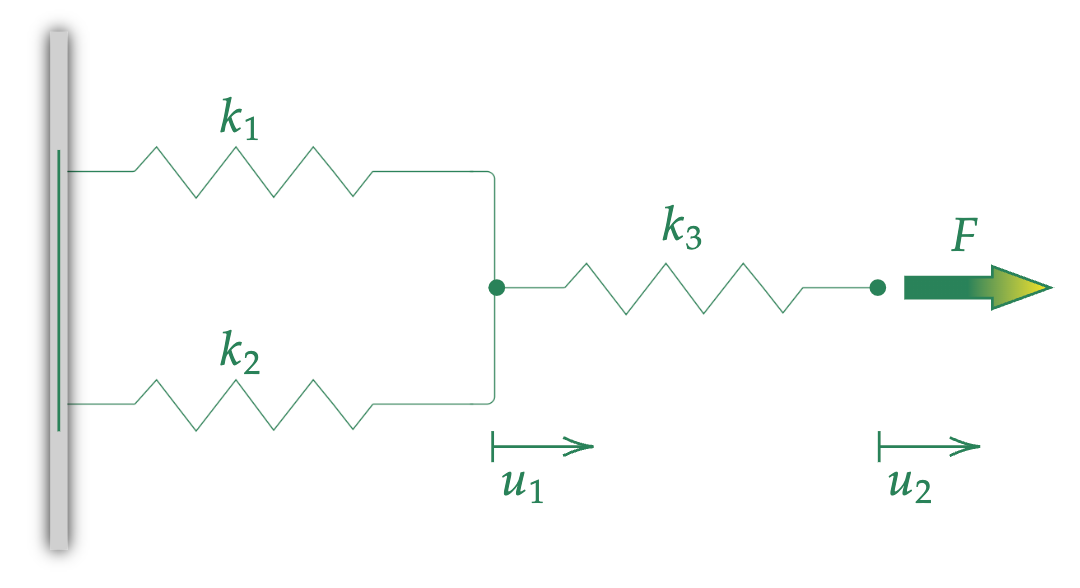
\includegraphics[width=0.8\textwidth]{spring_sys_2.png}
    \caption{System of nonlinear springs.}
    \label{fig:springs_first}
\end{figure}

The stiffness of the springs depends on the elongation of springs such that
\begin{equation}
\label{eq:spring_1}
k_i = k_i\left( e_i \right) = \alpha_i+\beta_i\cdot e_i\quad [\text{N/mm}],\qquad\qquad i=1,2,3,
\end{equation}
with $e_i$ being the elongation of the $i$-th spring and coefficients $\left( \alpha_i,\beta_i \right)$ being listed in Table~\ref{table:alpha_beta}. In this way, although the geometry of the problem is linear, it is ruled by nonlinear costitutive laws.

In Figure~\ref{fig:springs_first} is also shown the load application $F=100\ [\text{N}]$ at the tip.

Our interest lies in calculating $u_1$ and $u_2$, the nodal displacements at the two nodes.

\begin{table}[H]
    %\caption*{\textbf{Title of Table (optional)}}
    \centering 
    \begin{tabular}{ccc}
    \hline
    \rowcolor{bluepoli!40} % comment this line to remove the color
    $i$ & $\alpha_i$ & $\beta_i$  \\
    \hline
    1 & 500 & 50 \\
    2 & 200 & 100 \\
    3 & 500 & 100 \\
    \hline
    \end{tabular}
    \\[10pt]
    \caption{Springs coefficients.}
    \label{table:alpha_beta}
\end{table}

From Figure~\ref{fig:main13_1} one can notice that the stiffness (the local tangent) is increasing for increased elongations.

\begin{figure}[H]
    \centering
    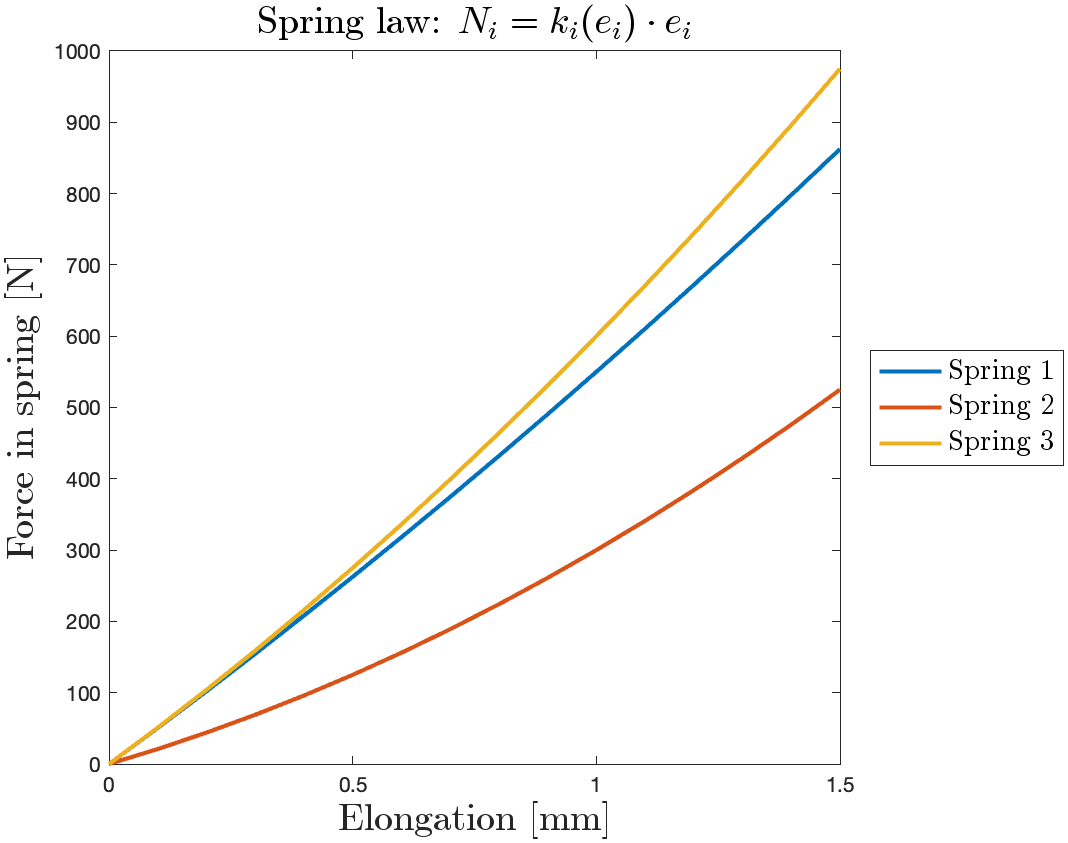
\includegraphics[width=0.9\textwidth]{main13_1.png}
    \caption{Costitutive law plot.}
    \label{fig:main13_1}
\end{figure}

Since springs 1 and 2 are fixed on the wall, their elongation is equivalent to $u_1$, while for spring 3, the elongation is $u_2-u_1$. It's very easy to find out the equilibrium of the two nodes:
\begin{equation}
\label{eq:spring_2}
\left\{
\begin{aligned}
N_1+N_2-N_3&=0, \\
N_3&=F.\\
\end{aligned}
\right.
\end{equation}

It follows that the matrix notation of the system in term of unknown displacement $u$ is
\begin{equation}
\label{eq:spring_25}
\mathbf{P}(\mathbf{u})=\mathbf{f}
\end{equation}
or, in a more physical notation,
\begin{equation}
\label{eq:spring_275}
\mathbf{F}^{\textbf{int}}(\mathbf{u})=\mathbf{F}^{\textbf{ext}},
\end{equation}

hence, the system is the following:
\begin{equation}
\label{eq:spring_3}
\left[
\begin{array}{cc}
 k_1+k_2+k_3 &-k_3 \\
 -k_3 & +k_3
\end{array}
\right]
\left[
\begin{array}{c}
 u_1 \\
 u_2
\end{array}
\right]
=
\left[
\begin{array}{c}
 0 \\
 F
\end{array}
\right].
\end{equation}

Note that, as we said before, the above equations are not linear as the stiffness matrix contains unknown variables.

Using the given stiffness of springs, the general matrix equation becomes
\begin{equation}
\label{eq:spring_4}
\begin{cases}
\left( \beta_1+\beta_2-\beta_3 \right)u_1^2 +\left( \alpha_1+\alpha_2+\alpha_3 \right)u_1+2\beta_3u_1u_2-\alpha_3u_2-\beta_3u_2^2=0 \\
\beta_3u_1^2-\alpha_3u_1-2\beta_3u_1u_2+\alpha_3u_2+\beta_3u_2^2=F
\end{cases},
\end{equation}

which, for the sake of generality, leads to
\begin{equation}
\label{eq:spring_5}
\begin{cases}
\mathcal{A}u_1^2 +\mathcal{B}u_1+\mathcal{C}u_1u_2+\mathcal{D}u_2+\mathcal{E}u_2^2=0 \\
\mathcal{F}u_1^2 +\mathcal{G}u_1+\mathcal{H}u_1u_2+\mathcal{I}u_2+\mathcal{L}u_2^2=F
\end{cases}.
\end{equation}

In this way it will be easier to build the system in MATLAB, namely with
\begin{equation}
\label{eq:spring_6}
\left[
\begin{array}{ccccc}
\mathcal{A} & \mathcal{B} & \mathcal{C} & \mathcal{D} & \mathcal{E} \\
\mathcal{F} & \mathcal{G} & \mathcal{H} & \mathcal{I} & \mathcal{L}
\end{array}
\right]
\left[
\begin{array}{c}
u_1^2 \\
u_1 \\
u_1u_2 \\
u_2 \\
u_2^2
\end{array}
\right].
\end{equation}

Finally, the assembled system is
\begin{equation}
\label{eq:spring_7}
\begin{cases}
50u_1^2+1200u_1+200u_1u_2-500u_2-100u_2^2=0 \\
100u_1^2-500u_1-200u_1u_2+500u_2+100u_2^2=100
\end{cases}.
\end{equation}

In the following section, a method of solving the system of nonlinear equations is discussed.

\section{Numerical Solution}
\label{sec:numerical_solution1}%

Before discussing systems, it is important to understand the problem of numerical approximation of the zeros of a real-valued function of one variable, that is
\begin{equation}
\label{eq:spring_8}
\boxed{\text{Given }f:(a,b)\to\mathbb{R},\text{ find }\alpha\in\mathbb{R}\text{ s.t. }f(\alpha)=0}
\end{equation}

There are several iterative methods to solve this rootfinding problem, such as the bisection method, the chord method, the secant method, fixed point methods, etc. For a more complete treatment of these, see for example \cite{quarter}.

In the following we analyze another algorithm: the Newton's method, also known as the \textbf{Newton–Raphson method}.

Assuming that $f\in\mathcal{C}^1\big( (a,b) \big)$ and that $\alpha$ is a simple root of $f$, if we let
\begin{equation}
\label{eq:spring_9}
q_k=f' ( x^k ),\qquad\forall k\geq 0
\end{equation}
and assign the initial value $x^0$, we obtain the Newton scheme
\begin{equation}
\label{eq:spring_10}
x^{k+1}=x^k-\frac{f( x^k )}{q_k},\qquad k\geq 0.
\end{equation}

The idea is clarified by looking at the first-order series expansion of $f(x)$ in the neighborhood of $x^k$
\begin{equation}
\label{eq:spring_11}
f(x)\approx f ( x^k )+\left[\frac{\text{d}f}{\text{d}x}(x^k)\right](x-x^k) \qquad\ \xrightarrow[]{x=x^{k+1}} \qquad \text{Equation~\eqref{eq:spring_10}}
\end{equation}

and by Figure~\ref{fig:quart1}.

\begin{figure}[H]
    \centering
    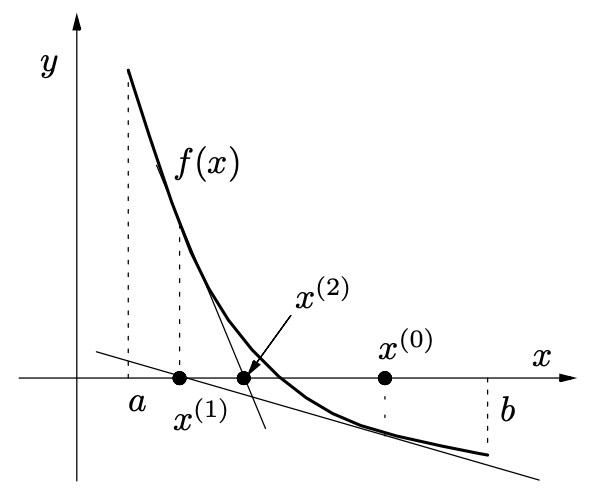
\includegraphics[width=0.5\textwidth]{quart1.png}
    \caption{Geometric approach of Newton-Raphson method: first two steps.}
    \label{fig:quart1}
\end{figure}

This method has an high order convergence, namely $p=2$, i.e.
\begin{equation}
\label{eq:spring_12}
\exists C>0\qquad\text{s.t.}\qquad \lim_{k\to\infty}\frac{\left| x^{k+1}-\alpha \right|}{\left| x^{k}-\alpha \right|^2}=C,
\end{equation}
but $\alpha$ should be a simple root and the initial value $x^0$ should be \emph{close} to the solution, because the method does not always guarantee convergence (actually, sometimes the solution may diverge or oscillate between two points). 

An immediate extension of Newton-Raphson’s method~\eqref{eq:spring_10} for the nonlinear system ~\eqref{eq:spring_25} can be recursively formulated as
\begin{equation}
\label{eq:spring_13}
\mathbf{u}^{k+1}=\mathbf{u}^k+\frac{ \mathbf{f}-\mathbf{P}(\mathbf{u}^k) }{\mathbf{K}_T^k}\qquad \text{with}\qquad \mathbf{K}_T^k=\frac{\partial\mathbf{P}}{\partial\mathbf{u}}(\mathbf{u}^k) ,
\end{equation}

which leads to the following algorithm:
\begin{subequations}
\label{eq:spring_14}
\begin{align}
\text{given }\mathbf{u}^0,\text{ for }k=&0,1,\dots,\text{ until convergence:} \nonumber \\
\text{compute}\qquad&\mathbf{K}_T^k\text{ and } \mathbf{R}^k=\mathbf{f}-\mathbf{P}(\mathbf{u}^k) , \label{eq:spring_15} \\
\text{solve}\qquad &\mathbf{K}_T^k\,\Delta\mathbf{u}^k=\mathbf{R}^k , \label{eq:spring_16} \\
\text{set}\qquad&\mathbf{u}^{k+1}=\mathbf{u}^k+\Delta\mathbf{u}^k. \label{eq:spring_17}
\end{align}
\end{subequations}

In general, this solution will not satisfy the system of nonlinear equations exactly and there will be some residual (or unbalance force in a physical point of view). If the $k$-th residual is smaller than a given tolerance, the solution $\mathbf{u}^{k+1}$ can be accepted as the accurate solution, and the process stops. The stopping criterion is expressed as follows
\begin{equation}
\label{eq:spring_18}
\text{conv}^{\,k+1}=\frac{\displaystyle\sum_{j=1}^n\left( \text{R}_j^{k+1} \right)^2}{1+\displaystyle\sum_{j=1}^n\left( \text{f}_j \right)^2},
\end{equation}
and, in order to show quadratic convergence as in Equation~\eqref{eq:spring_12}, it is often enough to show that $\textbf{conv}$ reduces quadratically at each iteration.

\smallskip

\begin{marker}
From Equation~\eqref{eq:spring_16}, one can notice that at each step $k$ the solution of a linear system with matrix $\mathbf{K}_T^k$ is required, thus the matrix cannot be singular. We will use the \emph{backslash} MATLAB command to solve the system, but the computational cost increases as $n^2$. There are several ways to solve this, for example use the LU decomposition and keep it fixed for some iterations, or just keep $\mathbf{K}_T^k$ fixed. See Secion~\ref{sec:numerical_implementation1} for further details.
\end{marker}

\newpage

\section{Numerical Implementation}
\label{sec:numerical_implementation1}%

Here we present and explain the MATLAB scripts used to solve the problem. The algorithms are listed in the Subsection~\ref{sub:matlab_scripts1}.

In \texttt{main11} (Algorithm~\ref{alg:main11}) we implement the Newton-Raphson method previously described. Here two auxiliary functions are used to compute the internal force vector $\mathbf{P}(\mathbf{u})$ and its Jacobian matrix $\mathbf{K}_T$ at each iteration. These MATLAB functions \newline
\texttt{generate\_int\_force} (Algorithm~\ref{alg:generate_int_force}) and \texttt{generate\_jacobian} (Algorithm~\ref{alg:generate_jacobian}) are merely based on Equation~\eqref{eq:spring_6}.

The output of the code is the following:
\begin{matlaboutput}
*********************************************************************
RESULTS
*********************************************************************

iter   u1        u2        conv
   0   2.00000   2.00000   4.00960e+02
   1   0.53846   0.73846   1.00124e+01
   2   0.16655   0.35914   4.30187e-02
   3   0.13889   0.33147   1.31776e-06
   4   0.13873   0.33132   1.29140e-15

Convergence reached in 4 iterations

*********************************************************************
\end{matlaboutput}

The initial guess choosen was $\mathbf{u}^0=[2;2]$, but we can easily repeat the process for other initial estimates. For example, with $\mathbf{u}^0=[0;0]$ we have 
\begin{matlaboutput}
*********************************************************************
RESULTS
*********************************************************************

iter   u1        u2        conv
   0   0.00000   0.00000   9.99900e-01
   1   0.14286   0.34286   1.68796e-03
   2   0.13874   0.33133   3.87449e-09
   3   0.13873   0.33132   1.81925e-20

Convergence reached in 3 iterations

*********************************************************************
\end{matlaboutput}

\newpage

and with $\mathbf{u}^0=[9;9]$ we have
\begin{matlaboutput}
*********************************************************************
RESULTS
*********************************************************************

iter   u1        u2        conv
   0   9.00000   9.00000   3.40378e+04
   1   3.60294   3.80294   1.90534e+03
   2   1.14953   1.34212   8.15108e+01
   3   0.28541   0.47799   1.25440e+00
   4   0.14284   0.33542   9.29483e-04
   5   0.13874   0.33132   6.38409e-10

Convergence reached in 5 iterations

*********************************************************************
\end{matlaboutput}

From all these outputs we can say that as MATLAB program iterates, the displacements converge to the numerical solution $\mathbf{u}=[0.13873;0.33132]$ mm; secondly, the number of iterations depends on the starting point, however the residual reduction via convergence criterion \eqref{eq:spring_18} is approximately quadratic.

We can double check the accuracy of our solution via plotting the surfaces of the system of nonlinear equations with zero-level contour. The results we obtain with \texttt{main12} (Algorithm~\ref{alg:main12}) ant the \texttt{plotzeros} function (Algorithm~\ref{alg:plotzeros}) are the following figures:
\begin{figure}[H]
    \centering
    \subfloat[Zero-level contour plot.\label{fig:main12_1}]{
        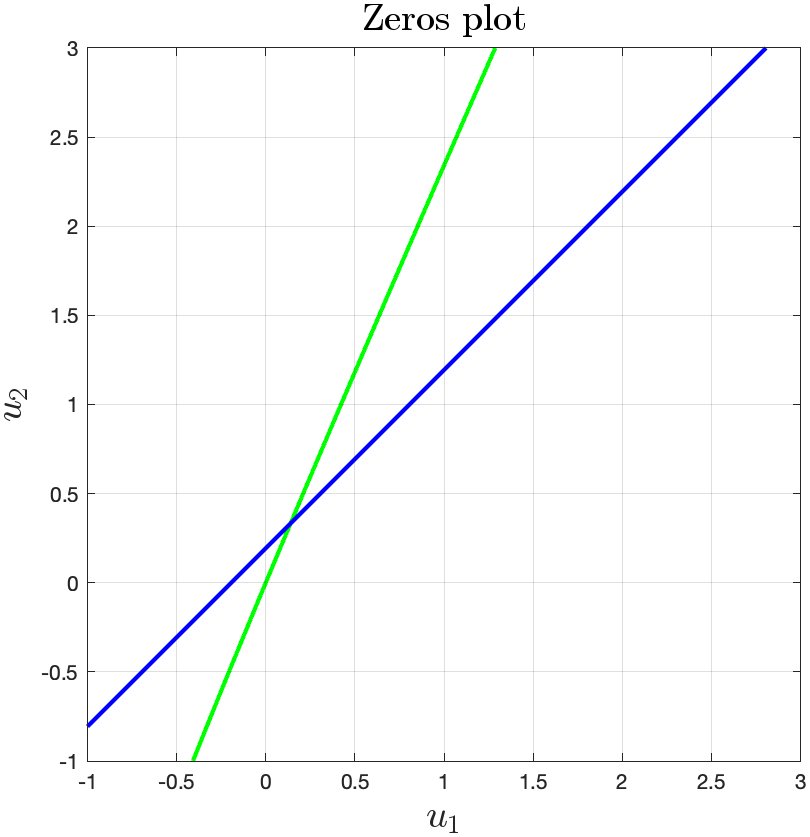
\includegraphics[scale=0.4]{Images/main12_1.png}
    }
    \quad
    \subfloat[3D Surface plot.\label{fig:main12_2}]{
        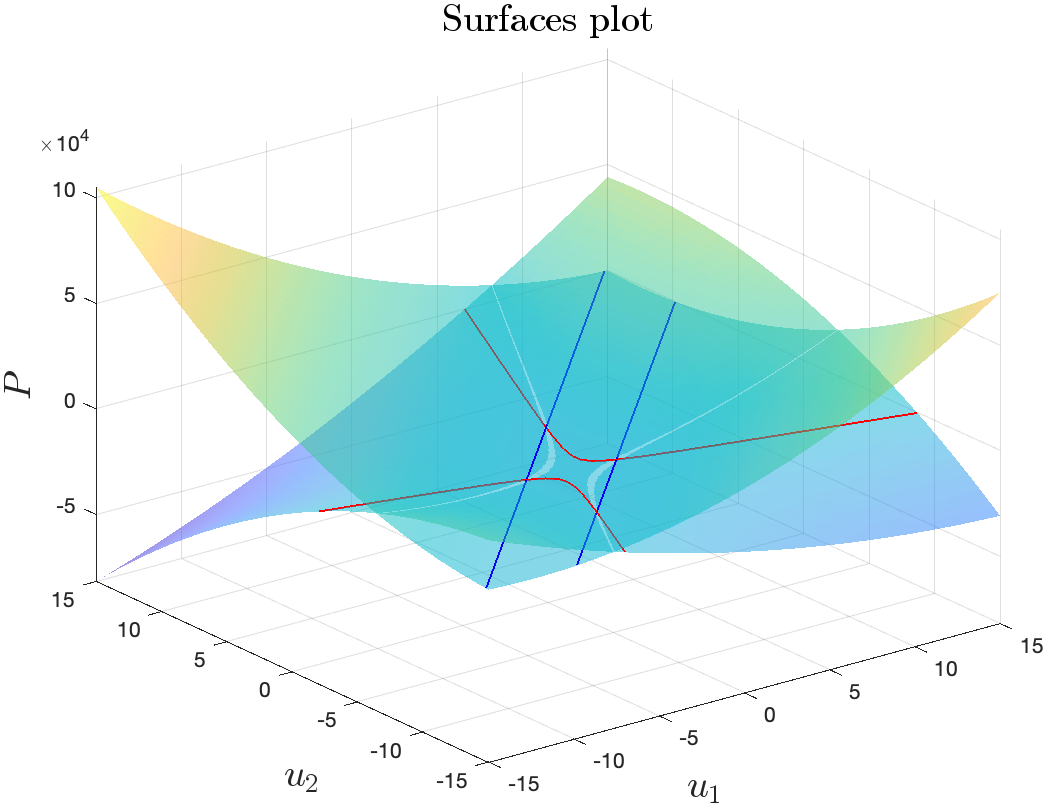
\includegraphics[scale=0.4]{Images/main12_2.png}
    }
    \caption{Zero-level contour and Surface plots.}
    \label{fig:main12}
\end{figure}

Note that there exist four solutions to the problem, but only one of them, the one we found, is positive.

\newpage

Thanks to script \texttt{main13} (Algorithm~\ref{alg:main13}) we generate useful data for the subsequent processing in Abaqus (see Section~\ref{sec:abaqus_implementation1}) and Figure~\ref{fig:main13_1}.

\vspace{5mm}

The Newton–Raphson method requires that at each iteration, the Jacobian matrix should be formed and the system of linearized equations should be solved for the increment of the solution. Computationally, these are expensive tasks. The \textbf{Modified Newton–Raphson method} is an attempt to make these procedures less expensive. Instead of formulating a new tangent stiffness matrix at each iteration, the initial tangent stiffness matrix is repeatedly used for all iterations. 

Through \texttt{main14} (Algorithm~\ref{alg:main14}) we implement the Modified Newton-Raphson method, gaining the following output:
\begin{matlaboutput}
*********************************************************************
RESULTS
*********************************************************************

iter   u1        u2        conv
   0   2.00000   2.00000   4.00960e+02
   1   0.53846   0.73846   1.00124e+01
   2   0.29199   0.48399   1.38037e+00
   3   0.20185   0.39448   2.24486e-01
   4   0.16538   0.35796   3.94896e-02
   5   0.15010   0.34268   7.13582e-03
   6   0.14360   0.33618   1.30509e-03
   7   0.14082   0.33340   2.39875e-04
   8   0.13963   0.33221   4.41837e-05
   9   0.13912   0.33170   8.14585e-06
  10   0.13890   0.33148   1.50238e-06
  11   0.13880   0.33139   2.77140e-07
  12   0.13876   0.33135   5.11268e-08
  13   0.13875   0.33133   9.43218e-09
  14   0.13874   0.33132   1.74013e-09
  15   0.13874   0.33132   3.21035e-10

Convergence reached in 15 iterations

*********************************************************************
\end{matlaboutput}

The method usually requires a greater number of iterations for convergence than that of the regular Newton–Raphson method. However, the overall computational cost to obtain the solution can be made less because each iteration is much faster than that of the regular Newton–Raphson method. The method is also a little more stable and is not prone to divergence.

\newpage

\subsection{MATLAB scripts}
\label{sub:matlab_scripts1}%

\begin{matlab}{main11}{alg:main11}
clear; clc; close;
% data
tol = 1.0e-9; iter = 0; max_iter = 100; u = [2;2]; old_u = u; F = 100;
a1 = 500; b1 = 50; a2 = 200; b2 = 100; a3 = 500; b3 = 100;
k1 = a1+b1*u(1); k2 = a2+b2*u(1); k3 = a3+b3*(u(2)-u(1));
% internal force vector
P = generate_int_force(u,a1,b1,a2,b2,a3,b3);
% external force vector
FF = [0; F];
% residual
R = FF - P;
% convergence parameter
conv = (R(1)^2+R(2)^2)/(1+FF(1)^2+FF(2)^2);
conv_rate = [];
fprintf('%s', repmat('*', 1, 69));
fprintf('\nRESULTS\n');
fprintf('%s', repmat('*', 1, 69));
fprintf('\n');
fprintf('\niter   u1        u2        conv');
fprintf('\n %3d   %7.5f   %7.5f   %7.5e',iter,u(1),u(2),conv);
while conv > tol && iter < max_iter
    % jacobian matrix of P
    Kt = generate_jacobian(u,a1,b1,a2,b2,a3,b3);
    % check if it is singular
    if det(Kt)==0
        fprintf('\n\n');
        error('Jacobian is singular!')
    end
    % solve the linear system
    delta_u = Kt\R;
    % update of the solution
    u = old_u + delta_u;
    % update of the internal force vector
    P = generate_int_force(u,a1,b1,a2,b2,a3,b3);
    % update of the residual
    R = FF - P;
    % update of the convergence parameter
    conv = (R(1)^2+R(2)^2)/(1+FF(1)^2+FF(2)^2);
    % save it in a vector
    conv_rate = [conv_rate; conv];
    % ready for a new iteration
    old_u = u;


    iter = iter + 1;
    % print of the results
    fprintf('\n %3d   %7.5f   %7.5f   %7.5e',iter,u(1),u(2),conv);
end
if iter==max_iter
    fprintf('\n\n');
    error('Convergence not reached!')
end
fprintf('\n\nConvergence reached in %d iterations',iter); 
fprintf('\n\n');
fprintf('%s', repmat('*', 1, 69)); fprintf('\n\n');
% p = log2(conv_rate(1:end-1)./conv_rate(2:end));

\end{matlab}

\bigskip

\begin{matlab}{generate int force}{alg:generate_int_force}
function P = generate_int_force(u,a1,b1,a2,b2,a3,b3)
A = b1+b2-b3; B = a1+a2+a3; C = 2*b3; D = -a3; E = -b3;
F = b3; G = -a3; H = -2*b3; I = a3; L = b3;
U = [u(1)^2;u(1);u(1)*u(2);u(2);u(2)^2];
P1 = [A,B,C,D,E;F,G,H,I,L];
P = P1*U;
end
\end{matlab}

\bigskip

\begin{matlab}{generate jacobian}{alg:generate_jacobian}
function J = generate_jacobian(u,a1,b1,a2,b2,a3,b3)
A = b1+b2-b3; B = a1+a2+a3; C = 2*b3; D = -a3; E = -b3;
F = b3; G = -a3; H = -2*b3; I = a3; L = b3;
U = [u(1);u(2);1];
J1 = [2*A,C,B;C,2*E,D;2*F,H,G;H,2*L,I];
J2 = J1*U;
J = [J2(1),J2(2);J2(3),J2(4)];
end
\end{matlab}

\newpage

\begin{matlab}{main12}{alg:main12}
clear; clc; close;
a1 = 500; b1 = 50; a2 = 200; b2 = 100; a3 = 500; b3 = 100; f = 100;
A = b1+b2-b3; B = a1+a2+a3; C = 2*b3; D = -a3; E = -b3;
F = b3; G = -a3; H = -2*b3; I = a3; L = b3;
fun = @(u) [A*u(1)^2+B*u(1)+C*u(1)*u(2)+D*u(2)+E*u(2)^2;
            F*u(1)^2+G*u(1)+H*u(1)*u(2)+I*u(2)+L*u(2)^2-f];
plotzeros(fun, [-1 3], [-1 3])
%
figure()
[X,Y] = meshgrid(-15:.5:15);
Z1 = (b1+b2-b3)*X.^2+(a1+a2+a3)*X+2*b3*X.*Y-a3*Y-b3*Y.^2;
s1 = surf(X,Y,Z1,'FaceAlpha',0.5);
s1.EdgeColor = 'none';
xlabel('$u_1$','Interpreter','latex',FontSize=18)
ylabel('$u_2$','Interpreter','latex',FontSize=18)
zlabel('$P$','Interpreter','latex',FontSize=18)
title('Surfaces plot','Interpreter','latex',FontSize=18)
hold on
Z2 = b3*X.^2-a3*X-2*b3*X.*Y+a3*Y+b3*Y.^2-F;
s2 = surf(X,Y,Z2,'FaceAlpha',0.5);
s2.EdgeColor = 'none';
contour(X,Y,Z1, [0 0], 'r', 'LineWidth', 1);
contour(X,Y,Z2, [0 0], 'b', 'LineWidth', 1);
\end{matlab}

\bigskip

\begin{matlab}{plotzeros}{alg:plotzeros}
function plotzeros(fun, x_limits, y_limits, varargin)
if nargin > 3
    sample_len = varargin{1};
else
    sample_len = 500;
end
v_dis_x = linspace(x_limits(1), x_limits(2), sample_len);
v_dis_y = linspace(y_limits(1), y_limits(2), sample_len);
n_dis_x = length(v_dis_x);
n_dis_y = length(v_dis_y);
Z_1 = zeros(n_dis_y, n_dis_x);
Z_2 = zeros(n_dis_y, n_dis_x);
for i = 1:n_dis_x
    for j = 1:n_dis_y
        funz = fun([v_dis_x(i); v_dis_y(j)]); 
        Z_1(j,i) = funz(1); Z_2(j,i) = funz(2);
    end
end


contour(v_dis_x, v_dis_y, Z_1, [0 0], 'Linecolor',[0 1 0], 'Linewidth', 2)
hold on
contour(v_dis_x, v_dis_y, Z_2, [0 0], 'Linecolor',[0 0 1], 'Linewidth', 2)
axis equal
grid on
xlabel('$u_1$','Interpreter','latex',FontSize=18)
ylabel('$u_2$','Interpreter','latex',FontSize=18)
title('Zeros plot','Interpreter','latex',FontSize=18)
end
\end{matlab}

\bigskip

\begin{matlab}{main13}{alg:main13}
clear; clc; close; format shorte
U = 0:0.1:1.5; Ut = U'
a1 = 500; b1 = 50; a2 = 200; b2 = 100; a3 = 500; b3 = 100;
k1 = a1+b1*Ut; k2 = a2+b2*Ut; k3 = a3+b3*Ut; kEQ = k1+k2;
F1 = k1.*Ut;
figure(1)
plot(Ut,F1,'linewidth',2)
xlabel('Elongation [mm]','Interpreter','latex',FontSize=18)
ylabel('Force in spring [N]','Interpreter','latex',FontSize=18)
title('Spring law: $N_i=k_i(e_i)\cdot e_i$','Interpreter','latex',FontSize=18)
hold on
F2 = k2.*Ut;
plot(Ut,F2,'linewidth',2)
F3 = k3.*Ut;
plot(Ut,F3,'linewidth',2)
legend('Spring 1','Spring 2','Spring 3','Interpreter','latex',Location='eastoutside',FontSize=14)
F12 = kEQ.*Ut
figure(2)
plot(Ut,F12,'linewidth',2)
xlabel('Elongation [mm]','Interpreter','latex',FontSize=18)
ylabel('Force in spring [N]','Interpreter','latex',FontSize=18)
title('Spring law: $N_i=k_i(e_i)\cdot e_i$','Interpreter','latex',FontSize=18)
hold on
F3 = k3.*Ut
plot(Ut,F3,'linewidth',2)
legend('Spring 1+2','Spring 3','Interpreter','latex',Location='eastoutside',FontSize=14)
\end{matlab}

\newpage

\begin{matlab}{main14}{alg:main14}
clear; clc; close;
tol = 1.0e-9; iter = 0; max_iter = 100; u = [2;2]; old_u = u; F = 100;
a1 = 500; b1 = 50; a2 = 200; b2 = 100; a3 = 500; b3 = 100;
k1 = a1+b1*u(1); k2 = a2+b2*u(1); k3 = a3+b3*(u(2)-u(1));
P = generate_int_force(u,a1,b1,a2,b2,a3,b3);
% jacobian matrix of P: FIXED
Kt = generate_jacobian(u,a1,b1,a2,b2,a3,b3);
FF = [0; F];
R = FF - P;
conv = (R(1)^2+R(2)^2)/(1+FF(1)^2+FF(2)^2);
conv_rate = [];
fprintf('%s', repmat('*', 1, 69));
fprintf('\nRESULTS\n');
fprintf('%s', repmat('*', 1, 69));
fprintf('\n');
fprintf('\niter   u1        u2        conv');
fprintf('\n %3d   %7.5f   %7.5f   %7.5e',iter,u(1),u(2),conv);
while conv > tol && iter < max_iter
    delta_u = Kt\R;
    u = old_u + delta_u;
    P = generate_int_force(u,a1,b1,a2,b2,a3,b3);
    R = FF - P;
    conv = (R(1)^2+R(2)^2)/(1+FF(1)^2+FF(2)^2);
    conv_rate = [conv_rate; conv];
    old_u = u;
    iter = iter + 1;
    fprintf('\n %3d   %7.5f   %7.5f   %7.5e',iter,u(1),u(2),conv);
end
if iter==max_iter
    fprintf('\n\n');
    error('Convergence not reached!')
end
fprintf('\n\nConvergence reached in %d iterations',iter); 
fprintf('\n\n');
fprintf('%s', repmat('*', 1, 69)); fprintf('\n\n');
% p = log2(conv_rate(1:end-1)./conv_rate(2:end));
\end{matlab}

\newpage

\section{Abaqus Implementation}
\label{sec:abaqus_implementation1}%

Here we solve the problem through the Abaqus Software by using spring-like connectors. The adopted units of measure are mm and N in order to be consistent, as Abaqus requires.

Before starting, let's remark that our nonlinear system shown in Figure~\ref{fig:springs_first} can be semplified in a system of two serial connected springs:
\begin{figure}[H]
    \centering
    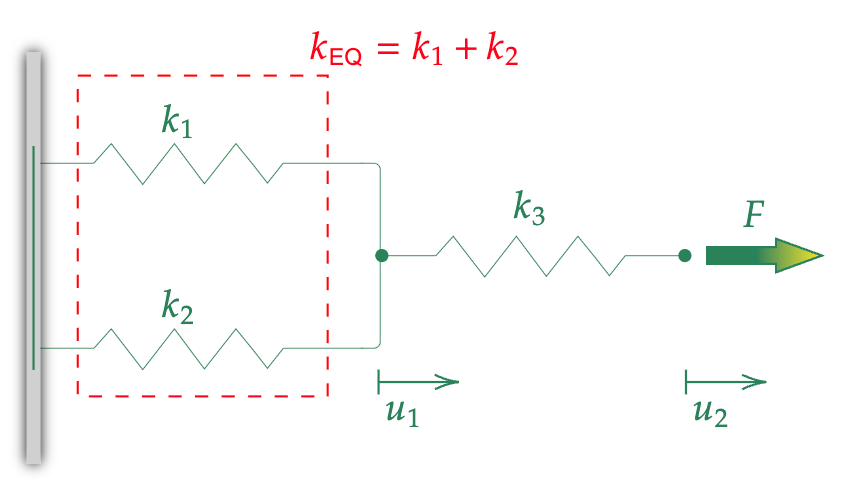
\includegraphics[width=0.5\textwidth]{spring_sys_3.png}
    \caption{Equivalent system of nonlinear springs.}
    \label{fig:springs_second}
\end{figure}

\subsection{Interaction module}
\label{interaction_module1}%

We define the nodes of the spring system by setting three colinear reference points (the distance between the nodes is not important) using the "Create Reference Point" button. Then we re-scale the view and the result is shown in Figure~\ref{fig:a2}.
\begin{figure}[H]
    \centering
    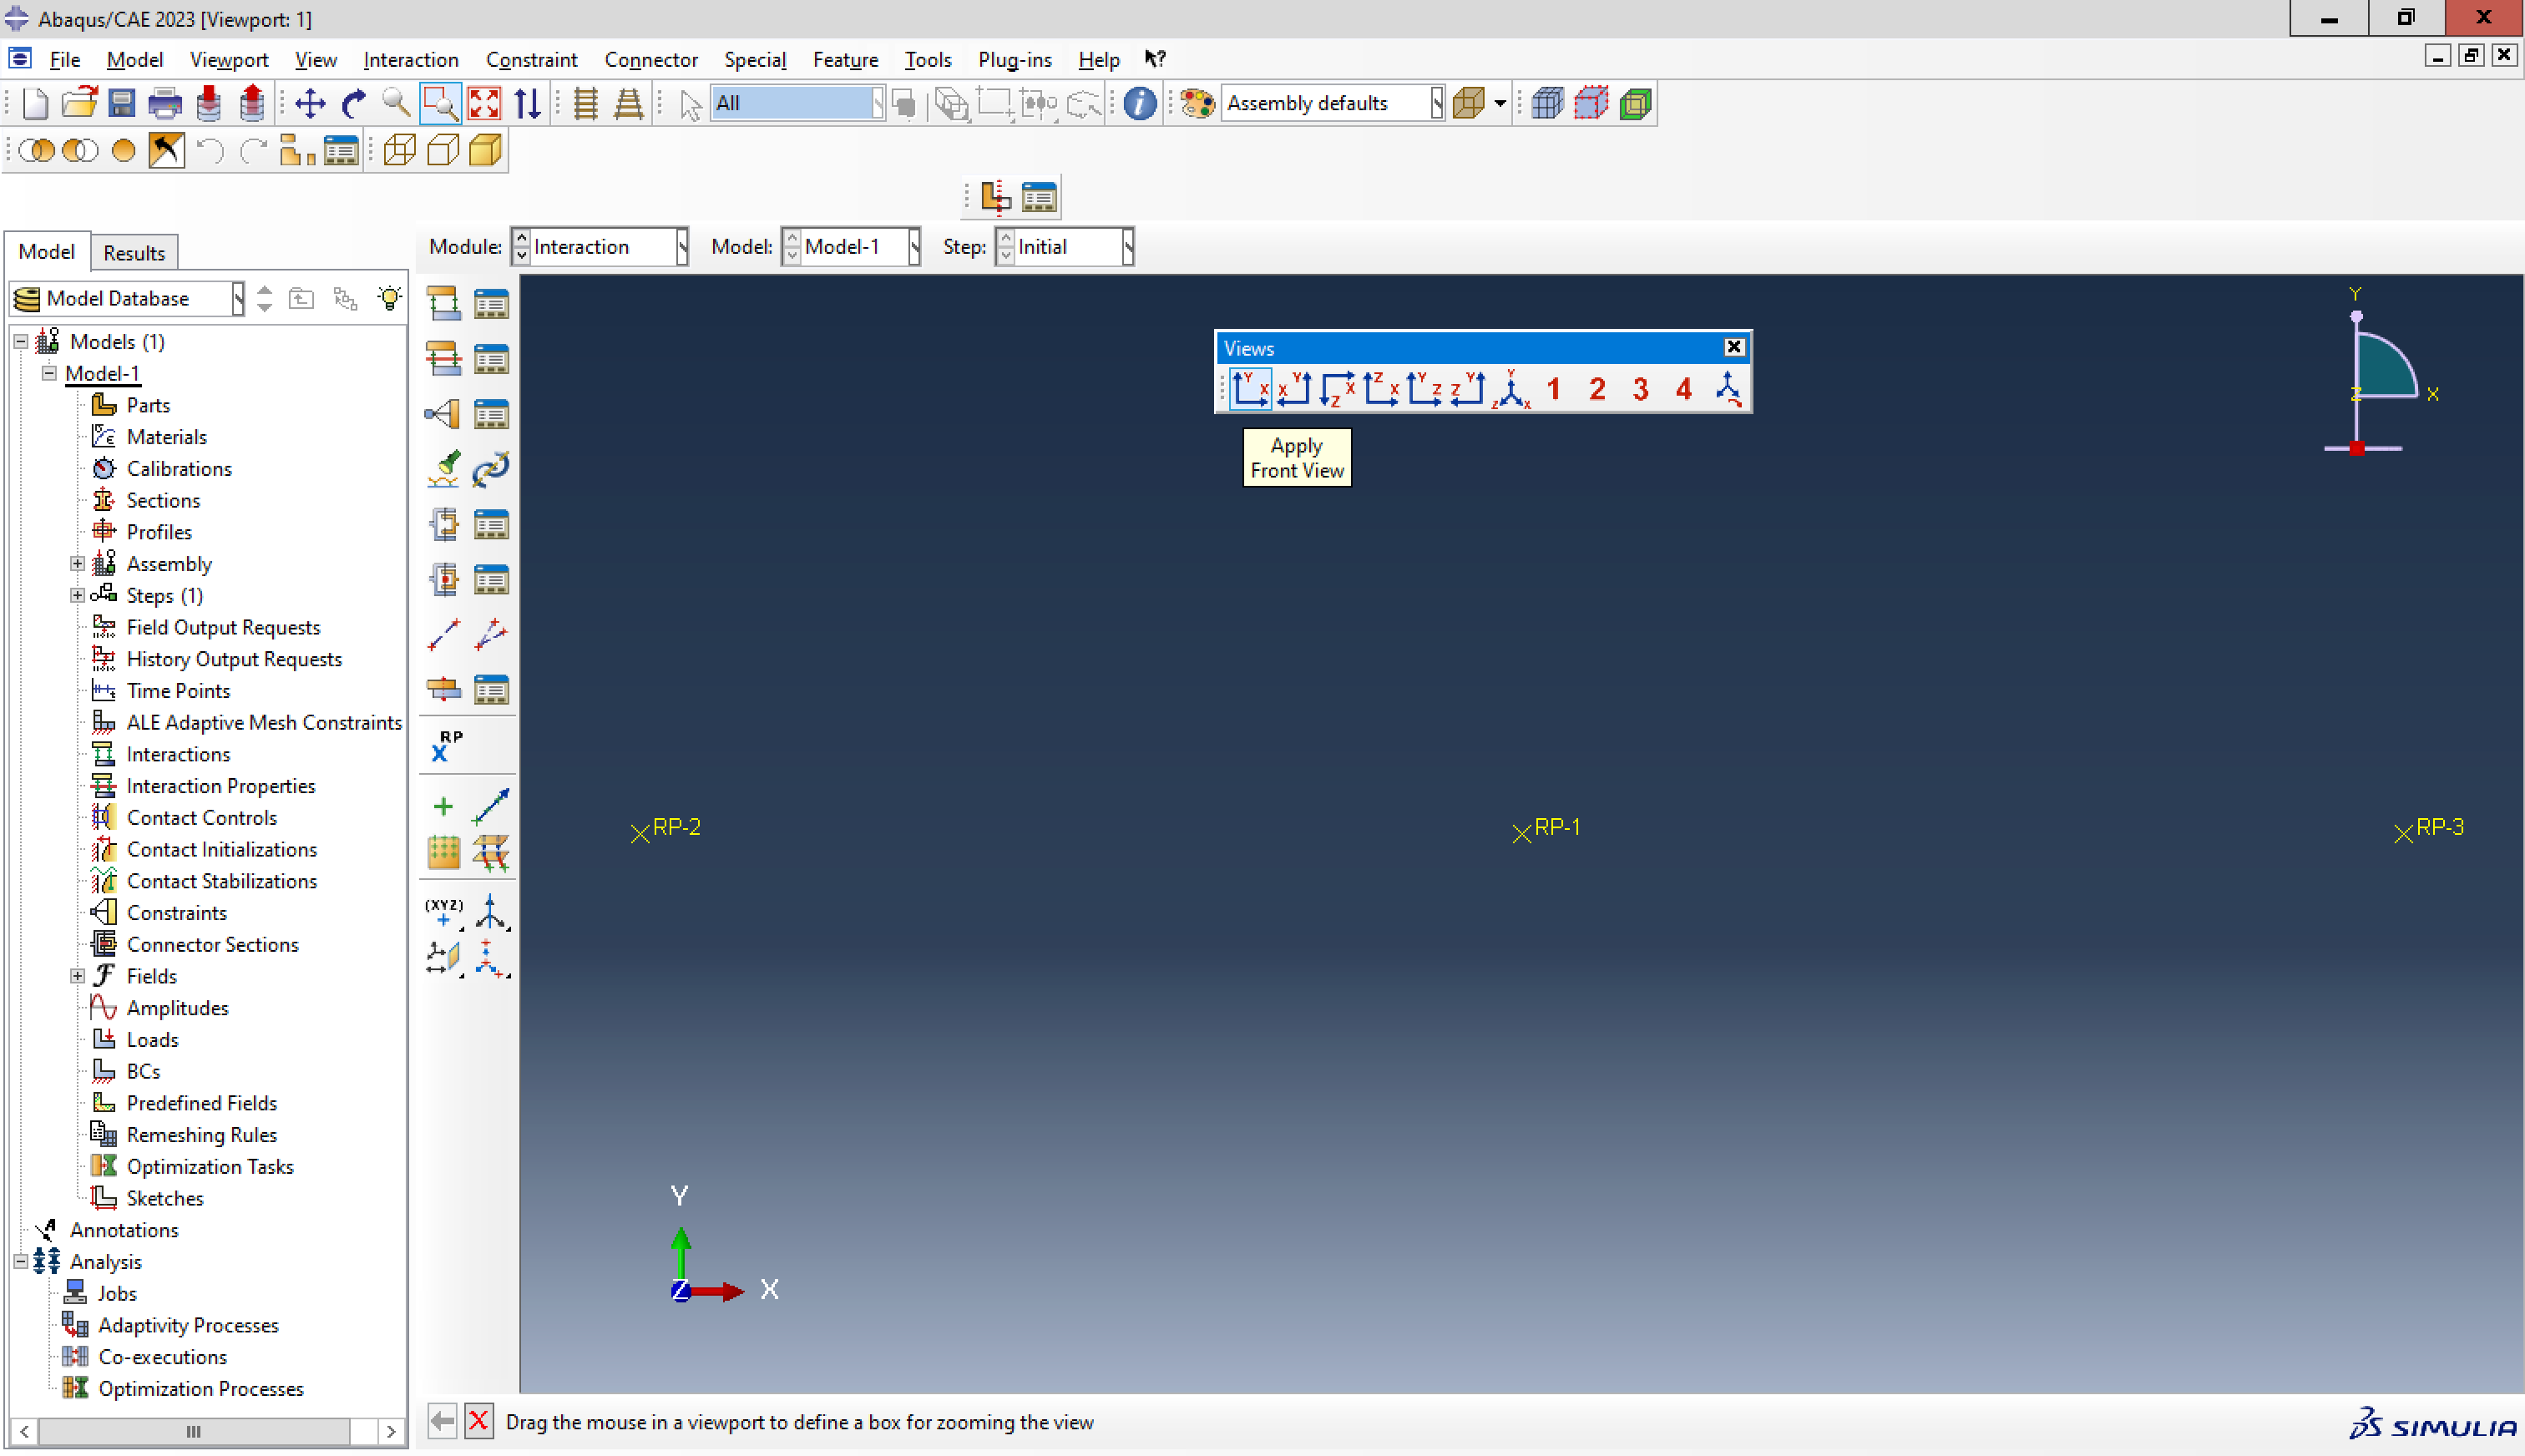
\includegraphics[width=0.9\textwidth]{Images/ab1/a2.png}
    \caption{Reference points.}
    \label{fig:a2}
\end{figure}

\newpage

We proceed by creating the wire feature by clicking on the "Create Wire Feature" 
\begin{figure}[H]
    \centering
    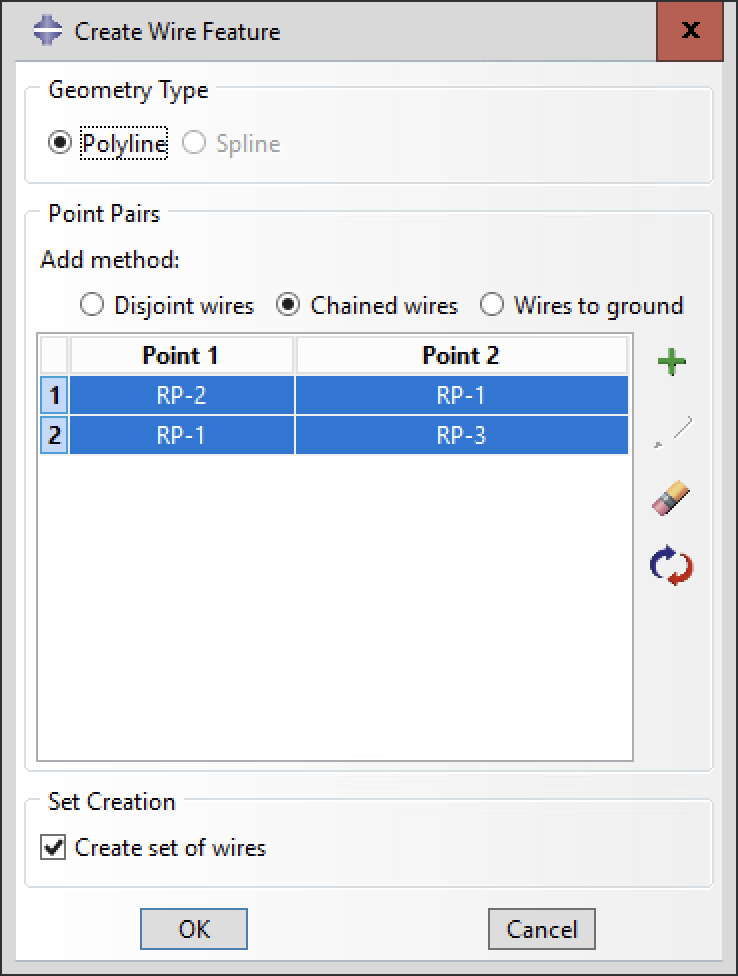
\includegraphics[width=0.4\textwidth]{Images/ab1/a4.png}
    \caption{Wire features.}
    \label{fig:a4}
\end{figure}

and the result is the following:
\begin{figure}[H]
    \centering
    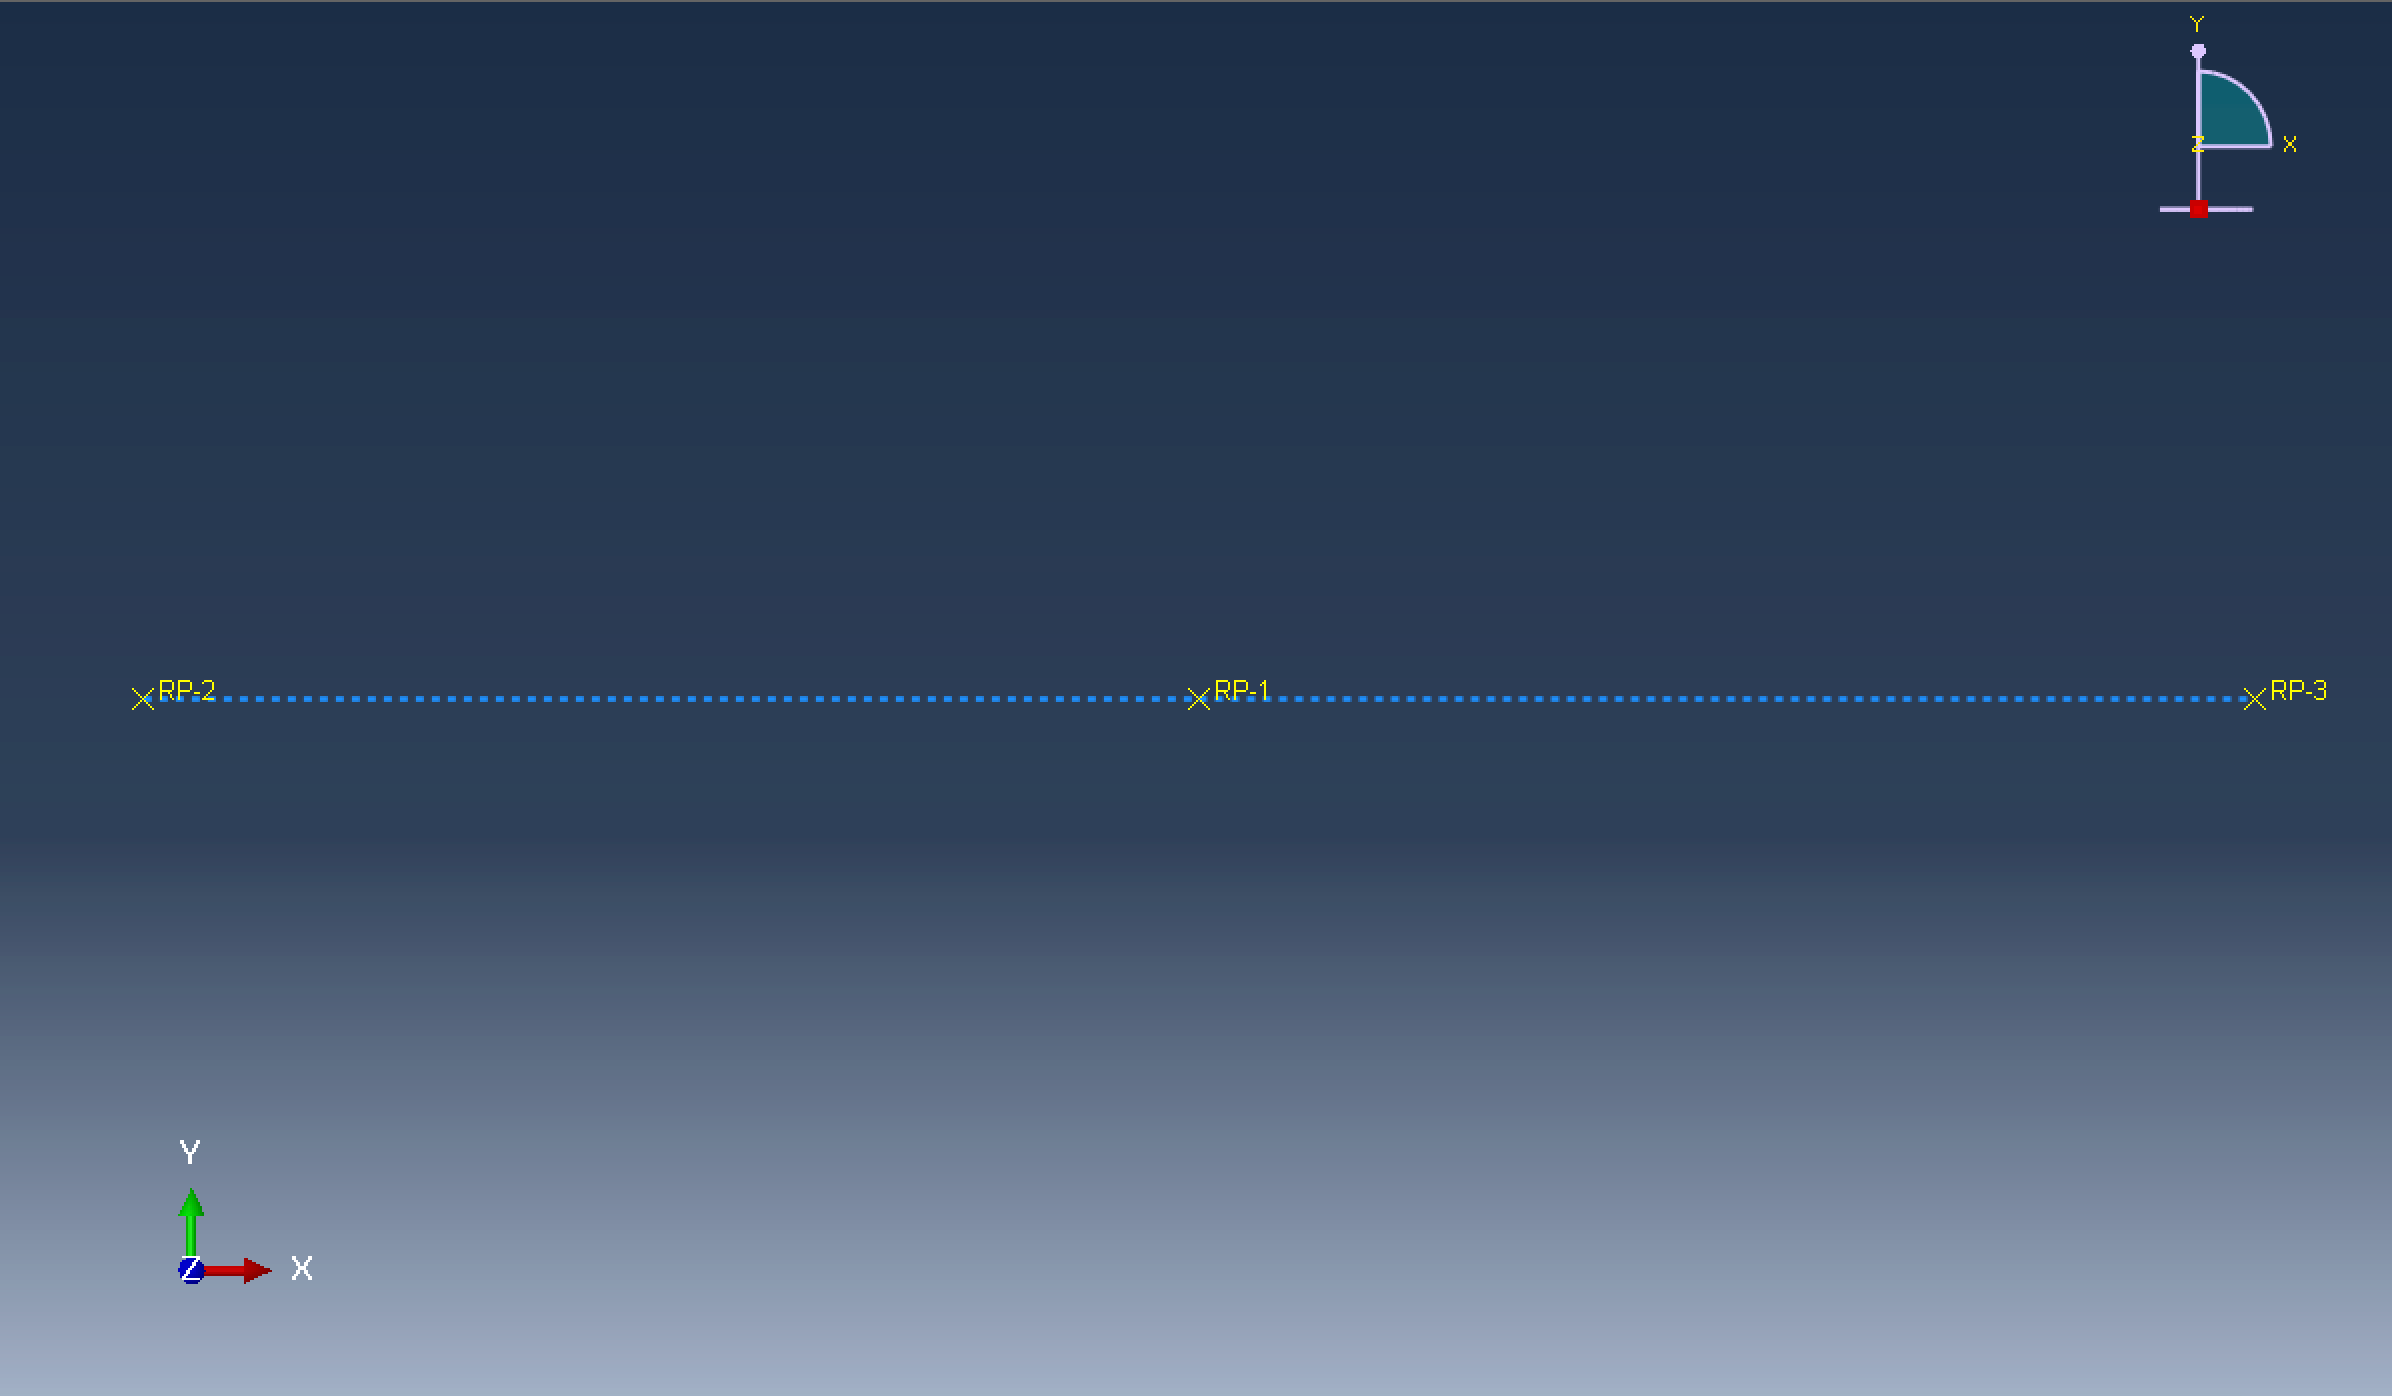
\includegraphics[width=0.9\textwidth]{Images/ab1/a5.png}
    \caption{Middle result of Interaction module.}
    \label{fig:a5}
\end{figure}

\newpage

A new \emph{section} should be defined for each springs. In the "Connector Section Manager", for both springs, we set the connection category as basic and the connection translational type as axial:
\begin{figure}[H]
    \centering
    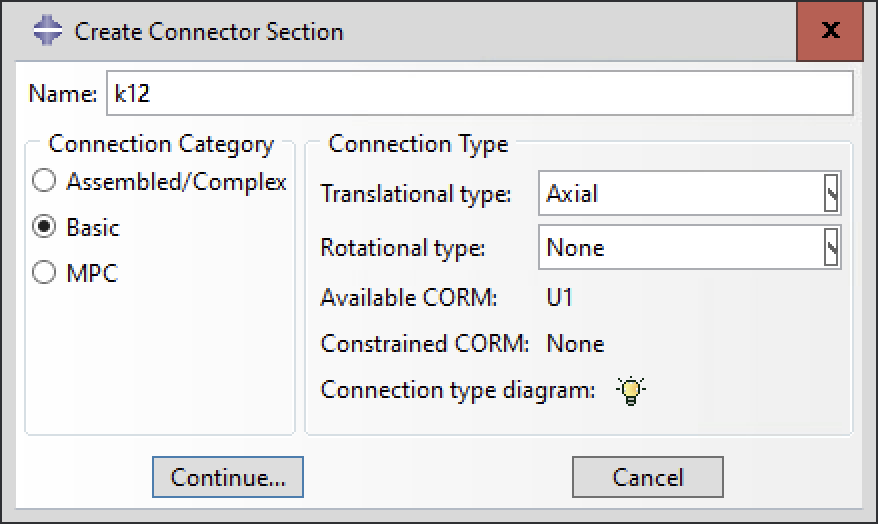
\includegraphics[width=0.4\textwidth]{Images/ab1/a7.png}
    \caption{Connector Section features.}
    \label{fig:a7}
\end{figure}

Here we manage to introduce nonlinearity by pasting the tables of values obtained with Algorithm~\ref{alg:main13} in MATLAB:
\begin{figure}[H]
    \centering
    \subfloat[Behavior options of Spring 1+2.\label{fig:a8}]{
        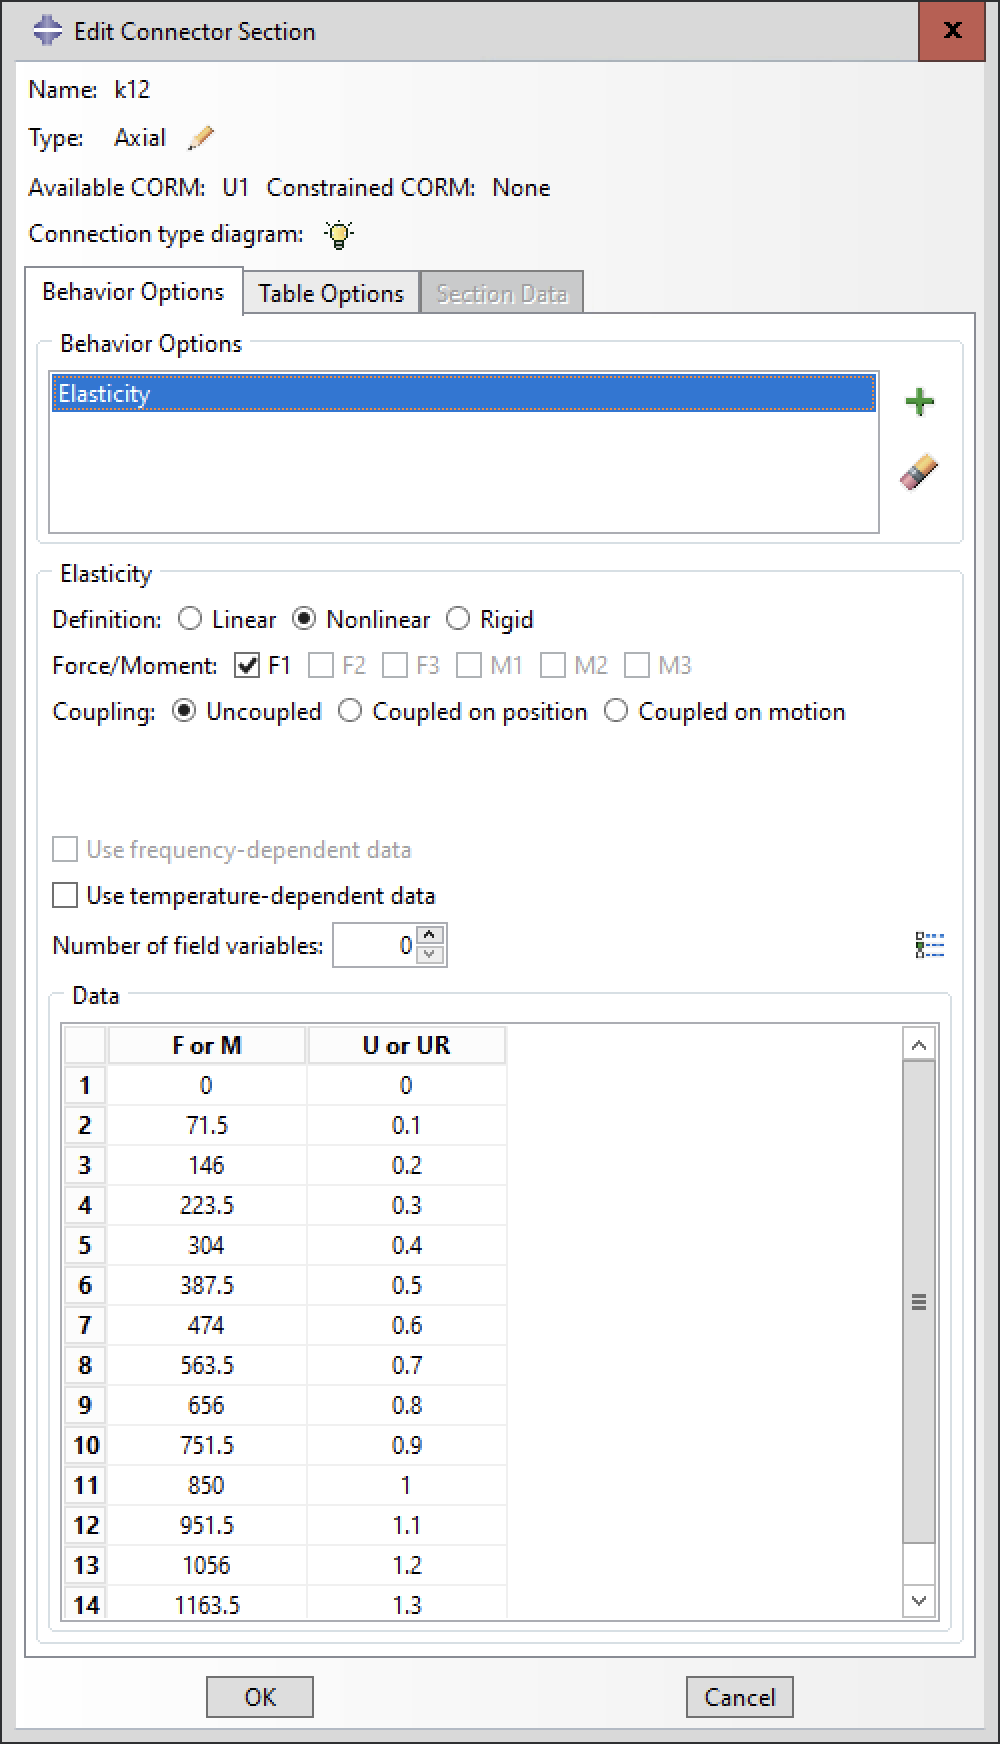
\includegraphics[scale=0.4]{Images/ab1/a8.png}
    }
    \quad
    \subfloat[Behavior options of Spring 3.\label{fig:a9}]{
        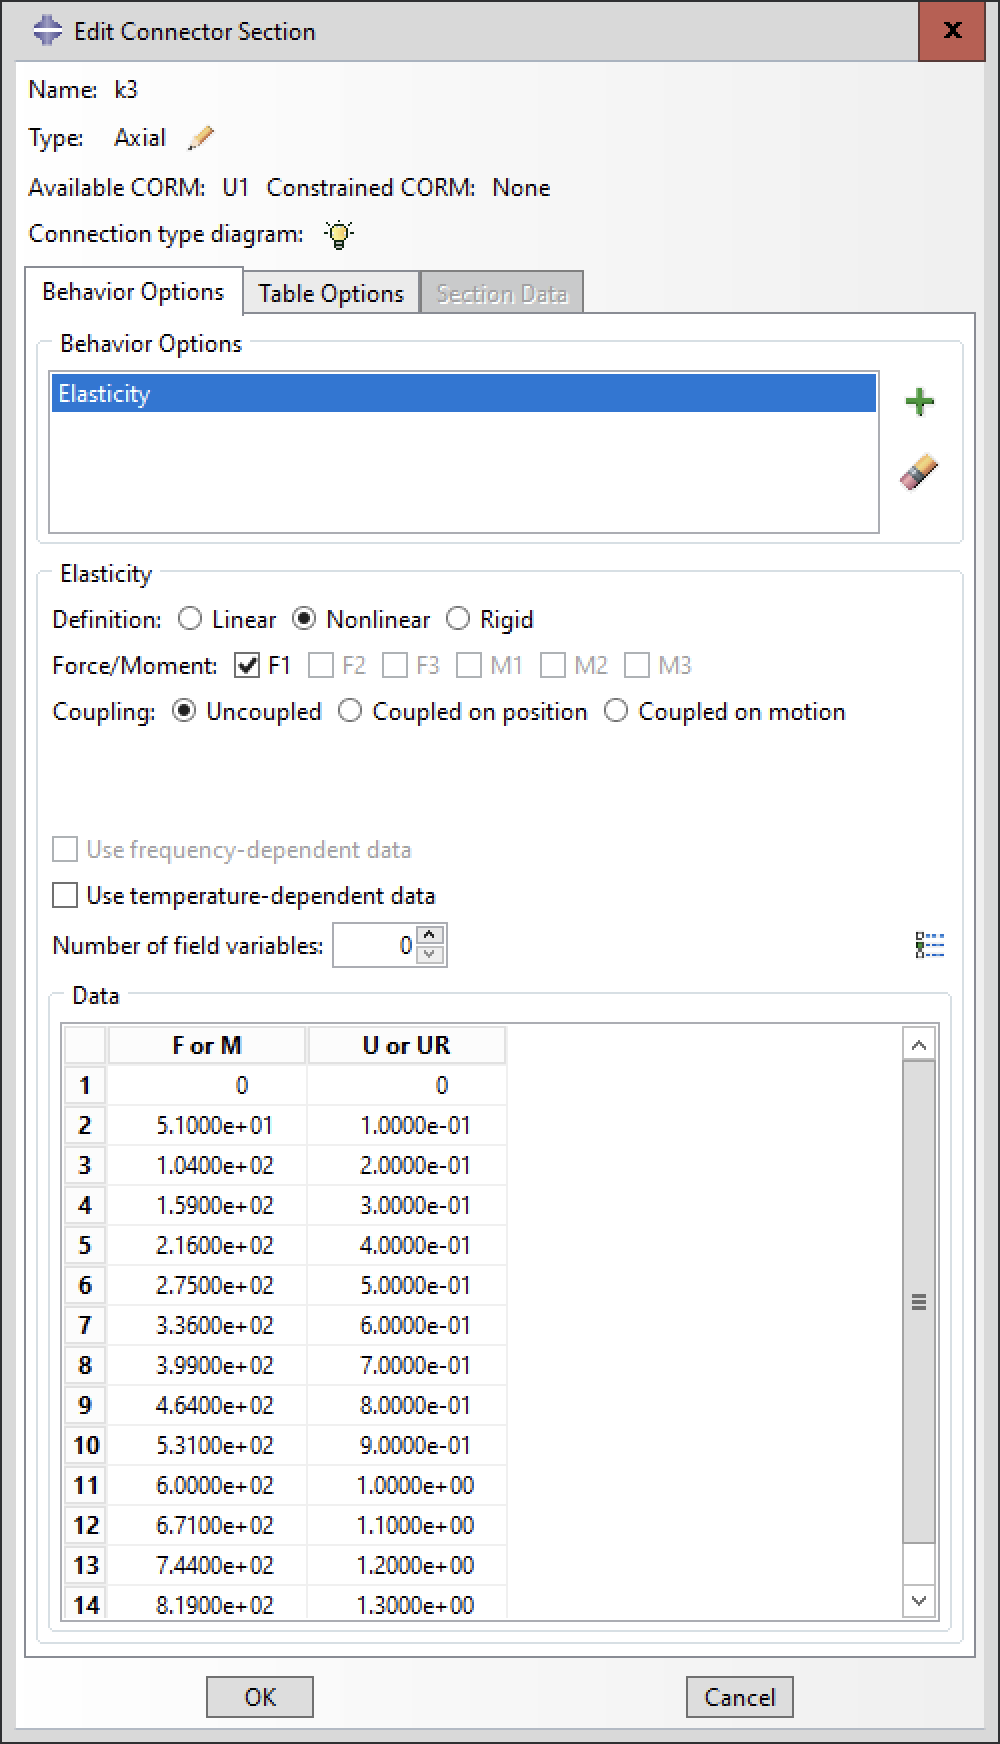
\includegraphics[scale=0.4]{Images/ab1/a9.png}
    }
    \caption{Behavior options of the springs.}
    \label{fig:a89}
\end{figure}

Finally, we associate each spring with its respective mechanical property:
\begin{figure}[H]
    \centering
    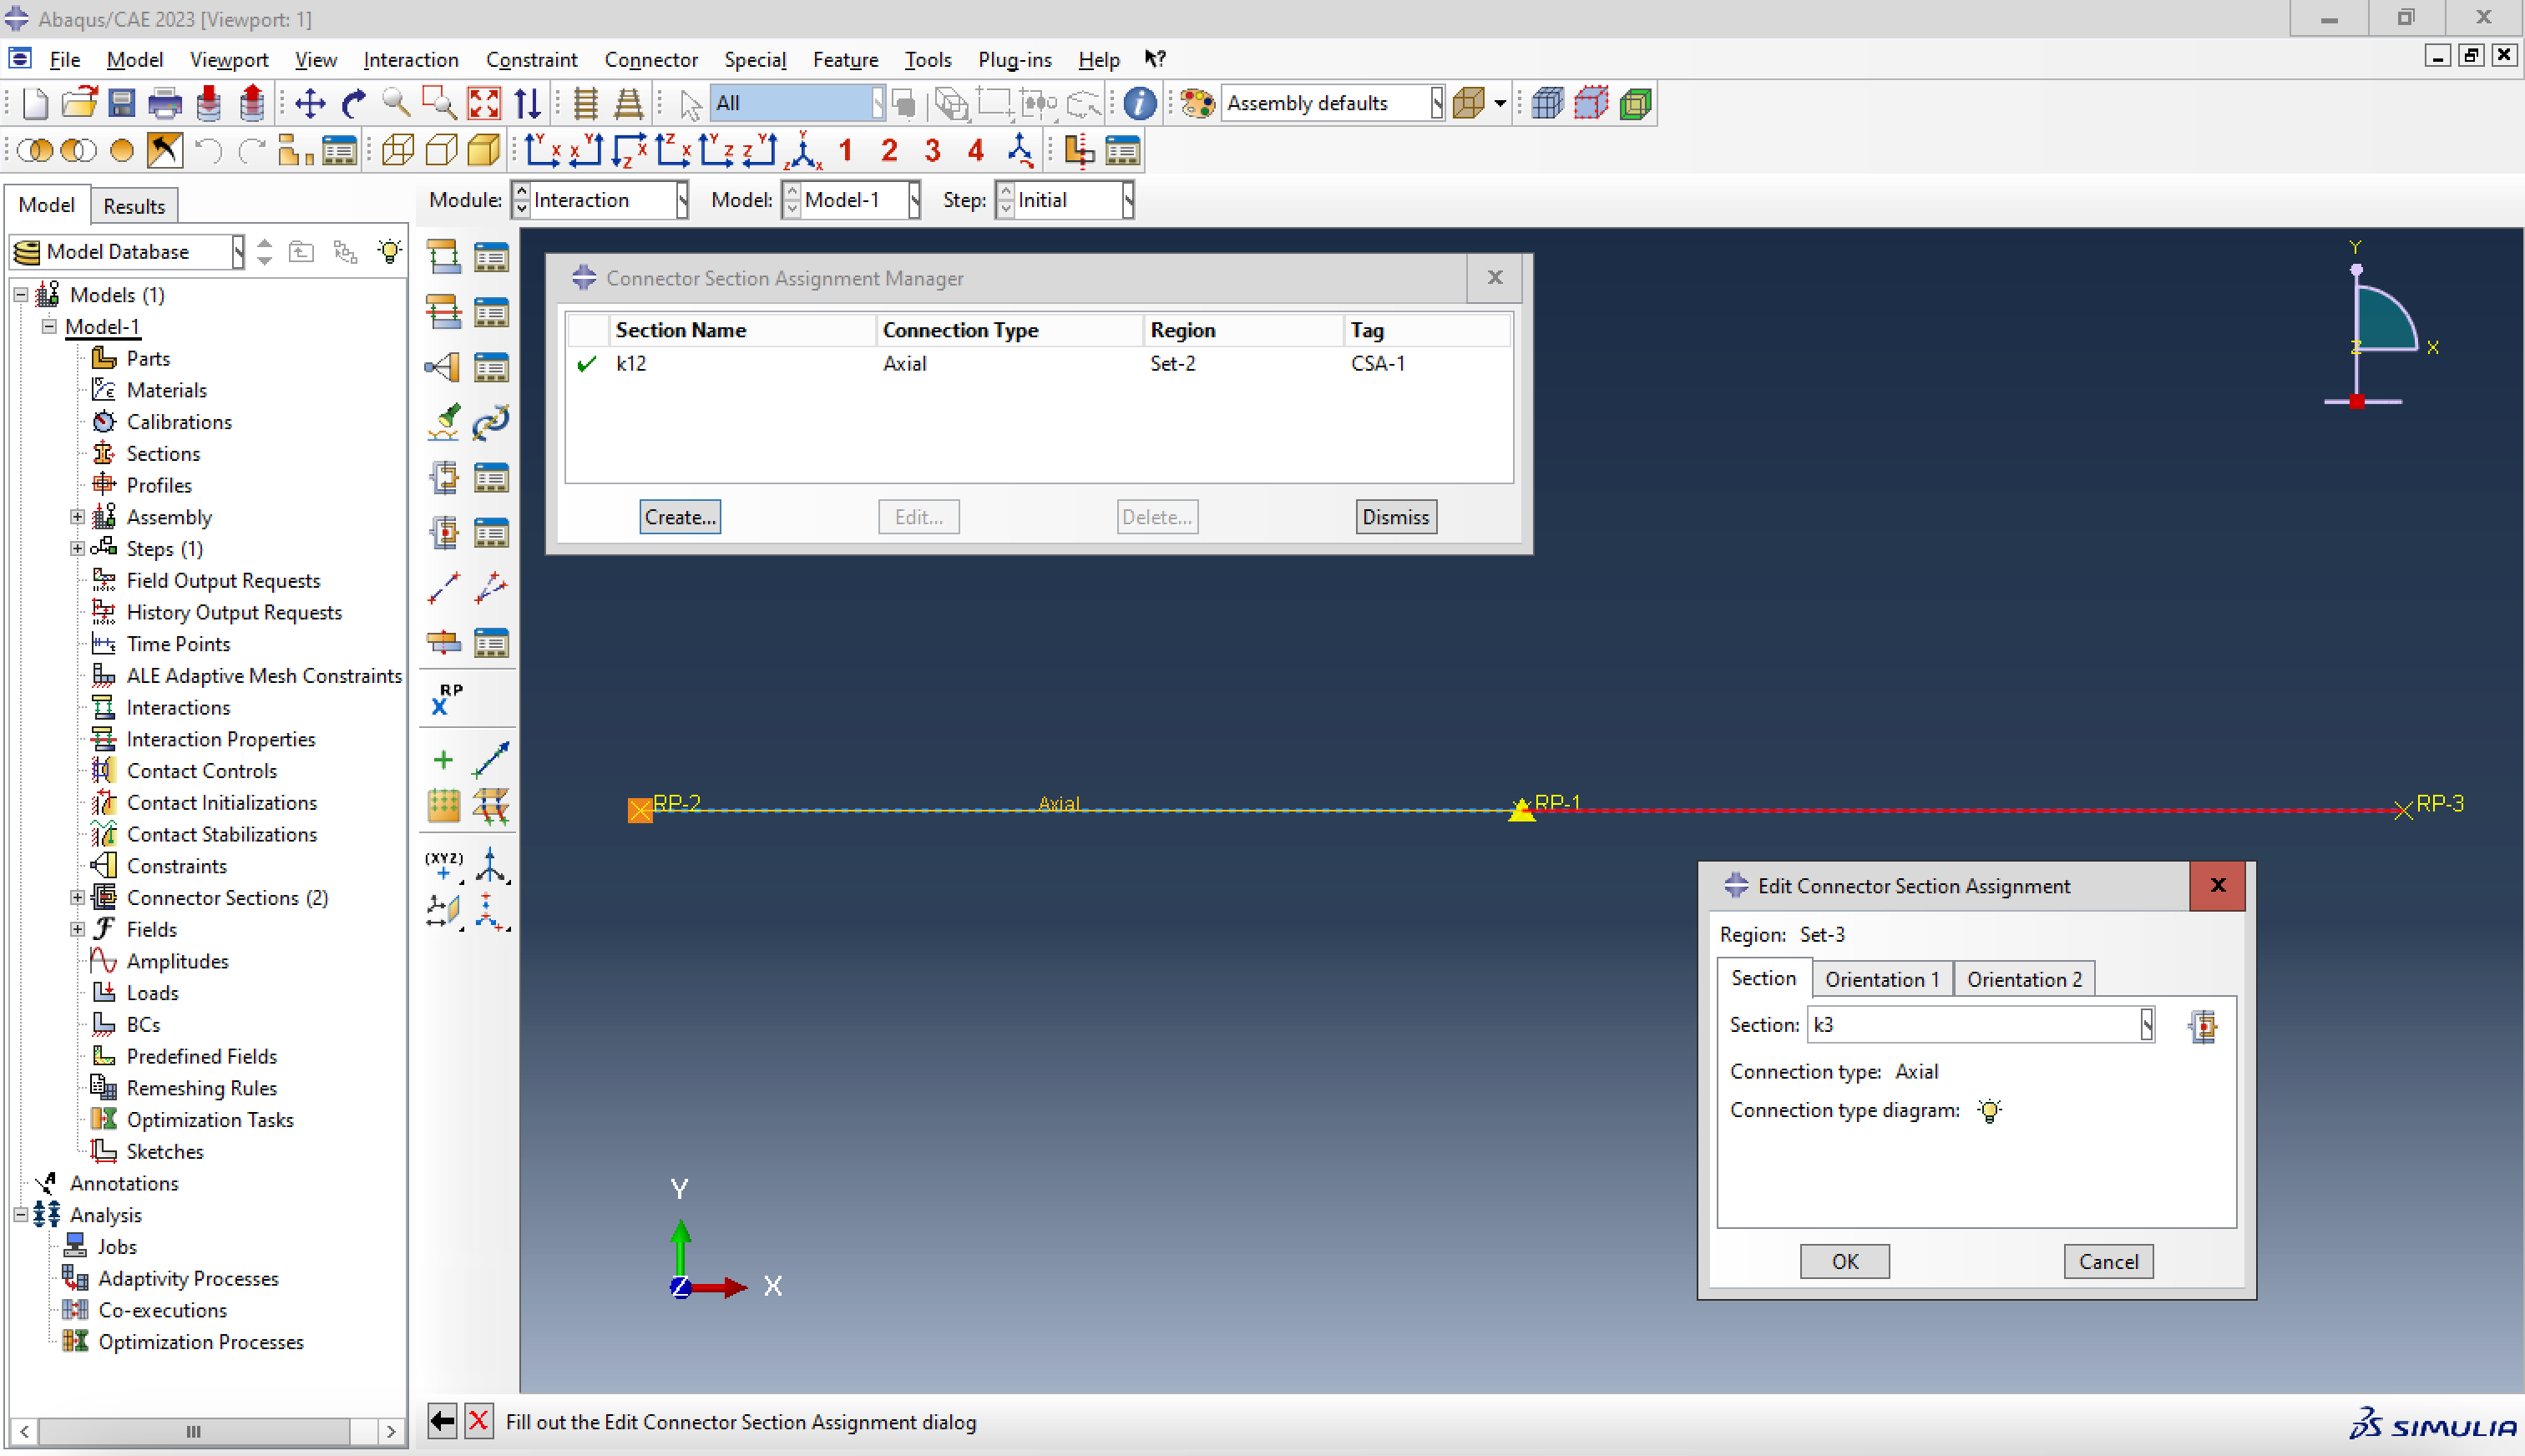
\includegraphics[width=0.9\textwidth]{Images/ab1/a10.png}
    \caption{Connector Section Assignment.}
    \label{fig:a10}
\end{figure}

The final result of this module is shown in Figure~\ref{fig:a11}.
\begin{figure}[H]
    \centering
    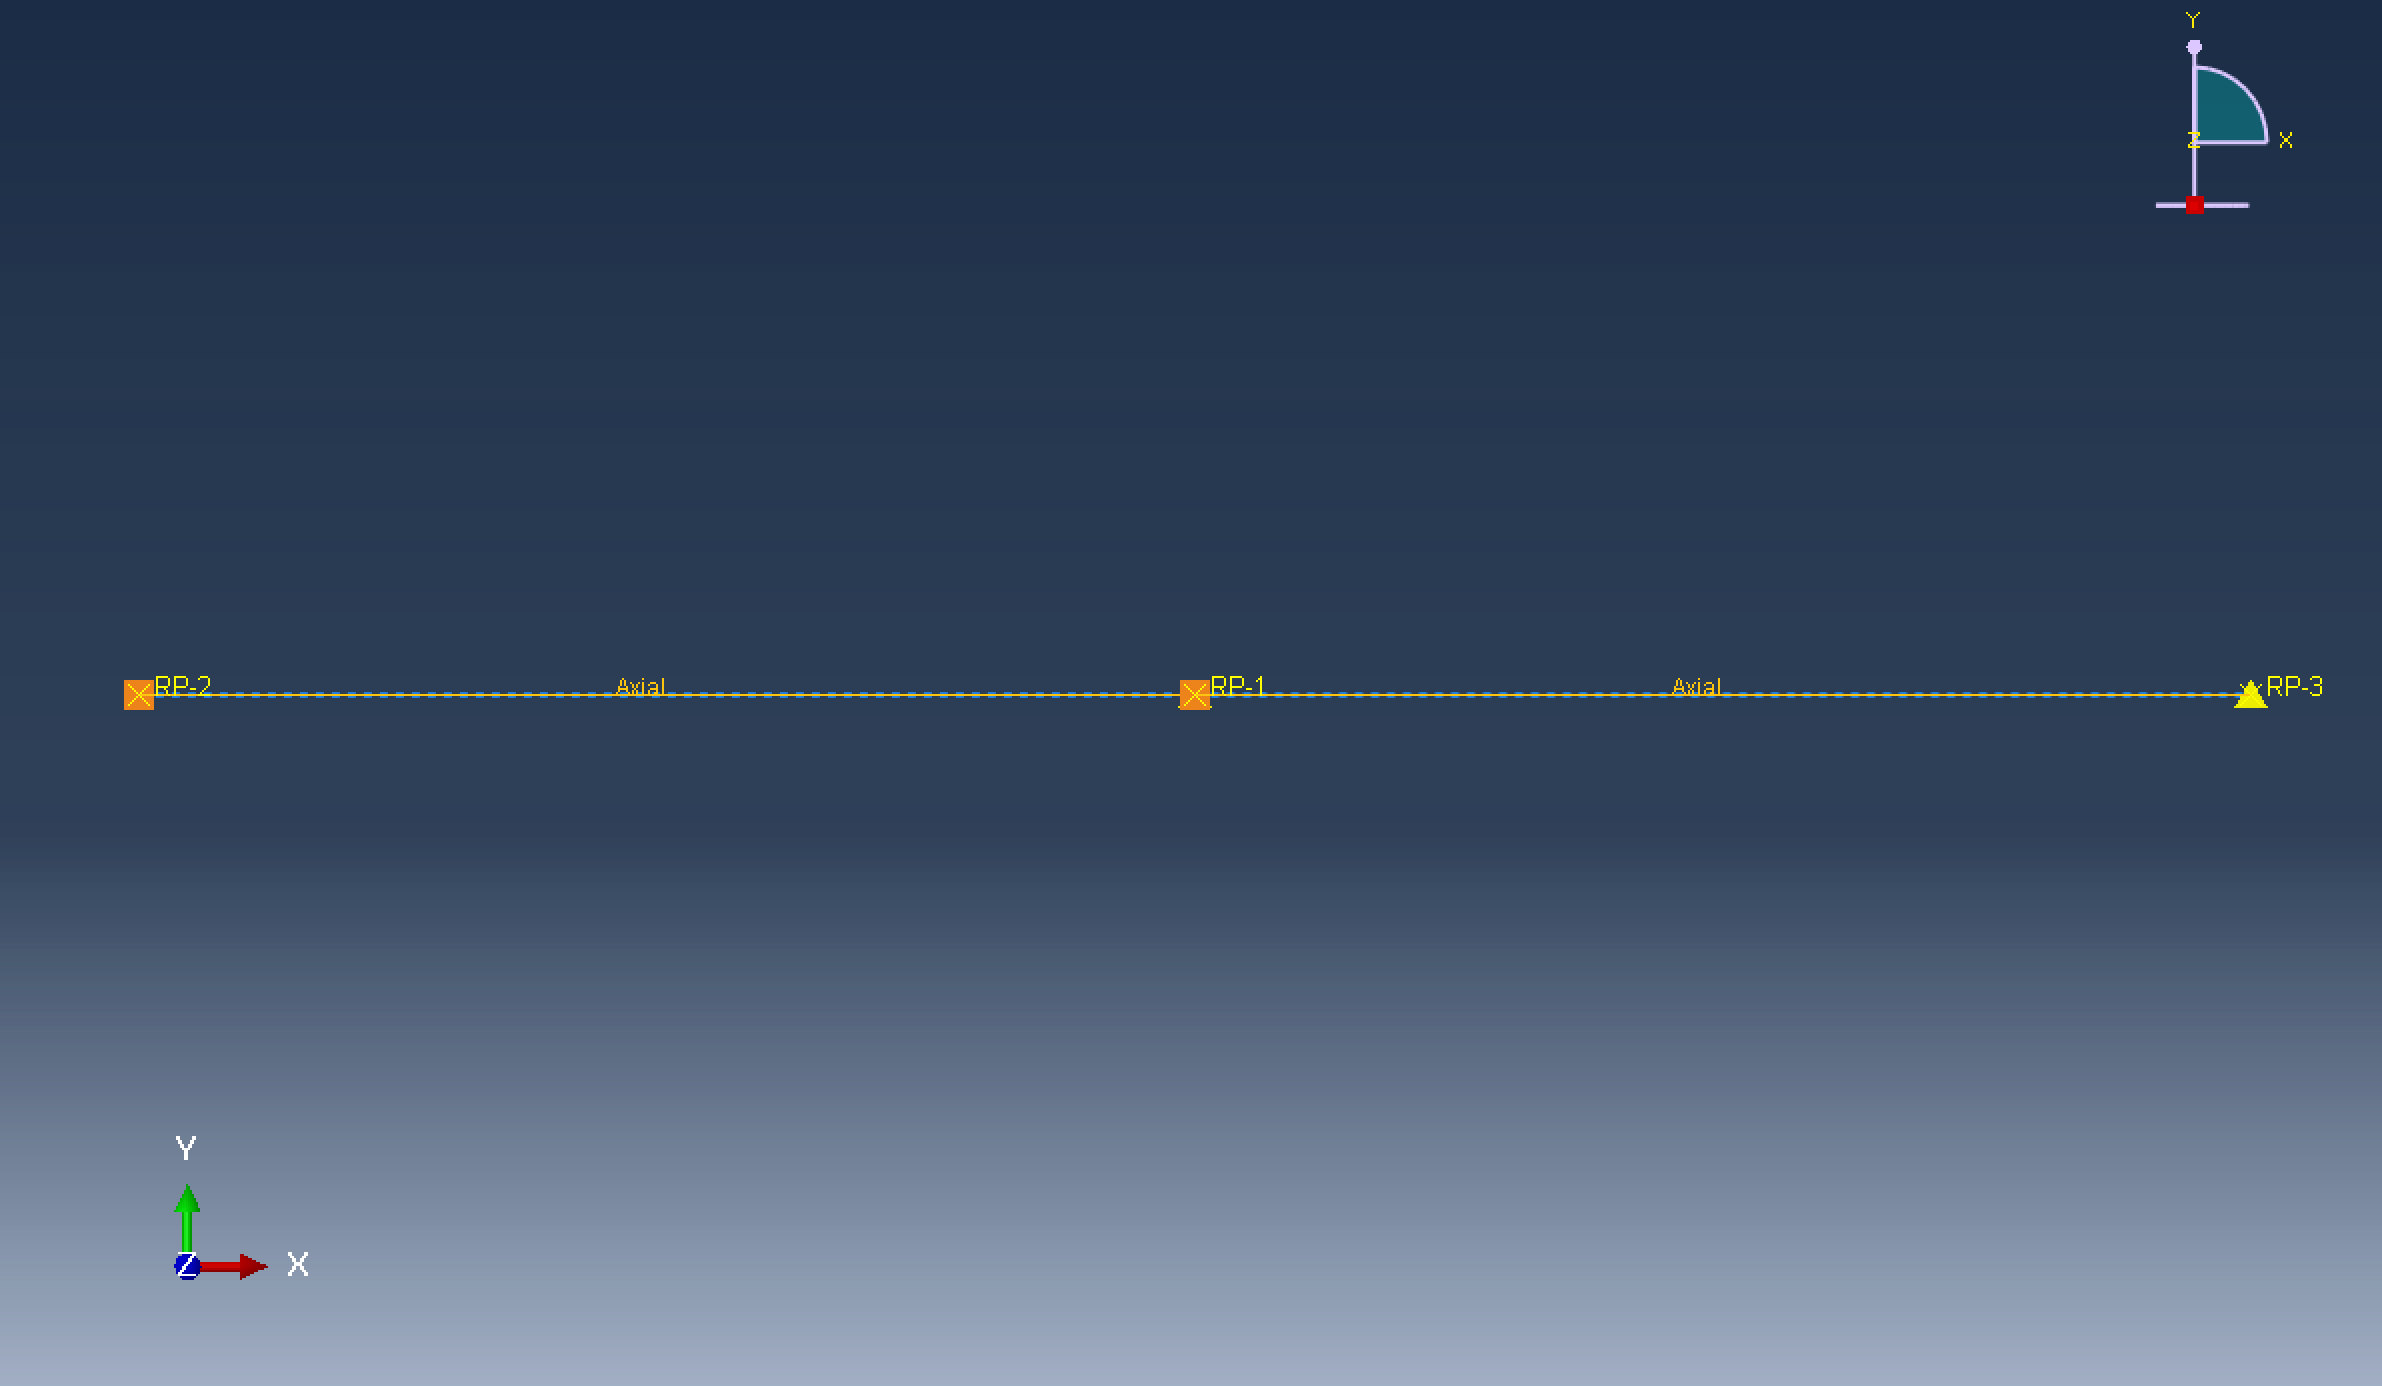
\includegraphics[width=0.9\textwidth]{Images/ab1/a11.png}
    \caption{Final result of Interaction module.}
    \label{fig:a11}
\end{figure} 

\newpage

\subsection{Step module}
\label{step_module1}%

We click on the "Step Manager" button, which looks like Figure~\ref{fig:a12},

\begin{figure}[H]
    \centering
    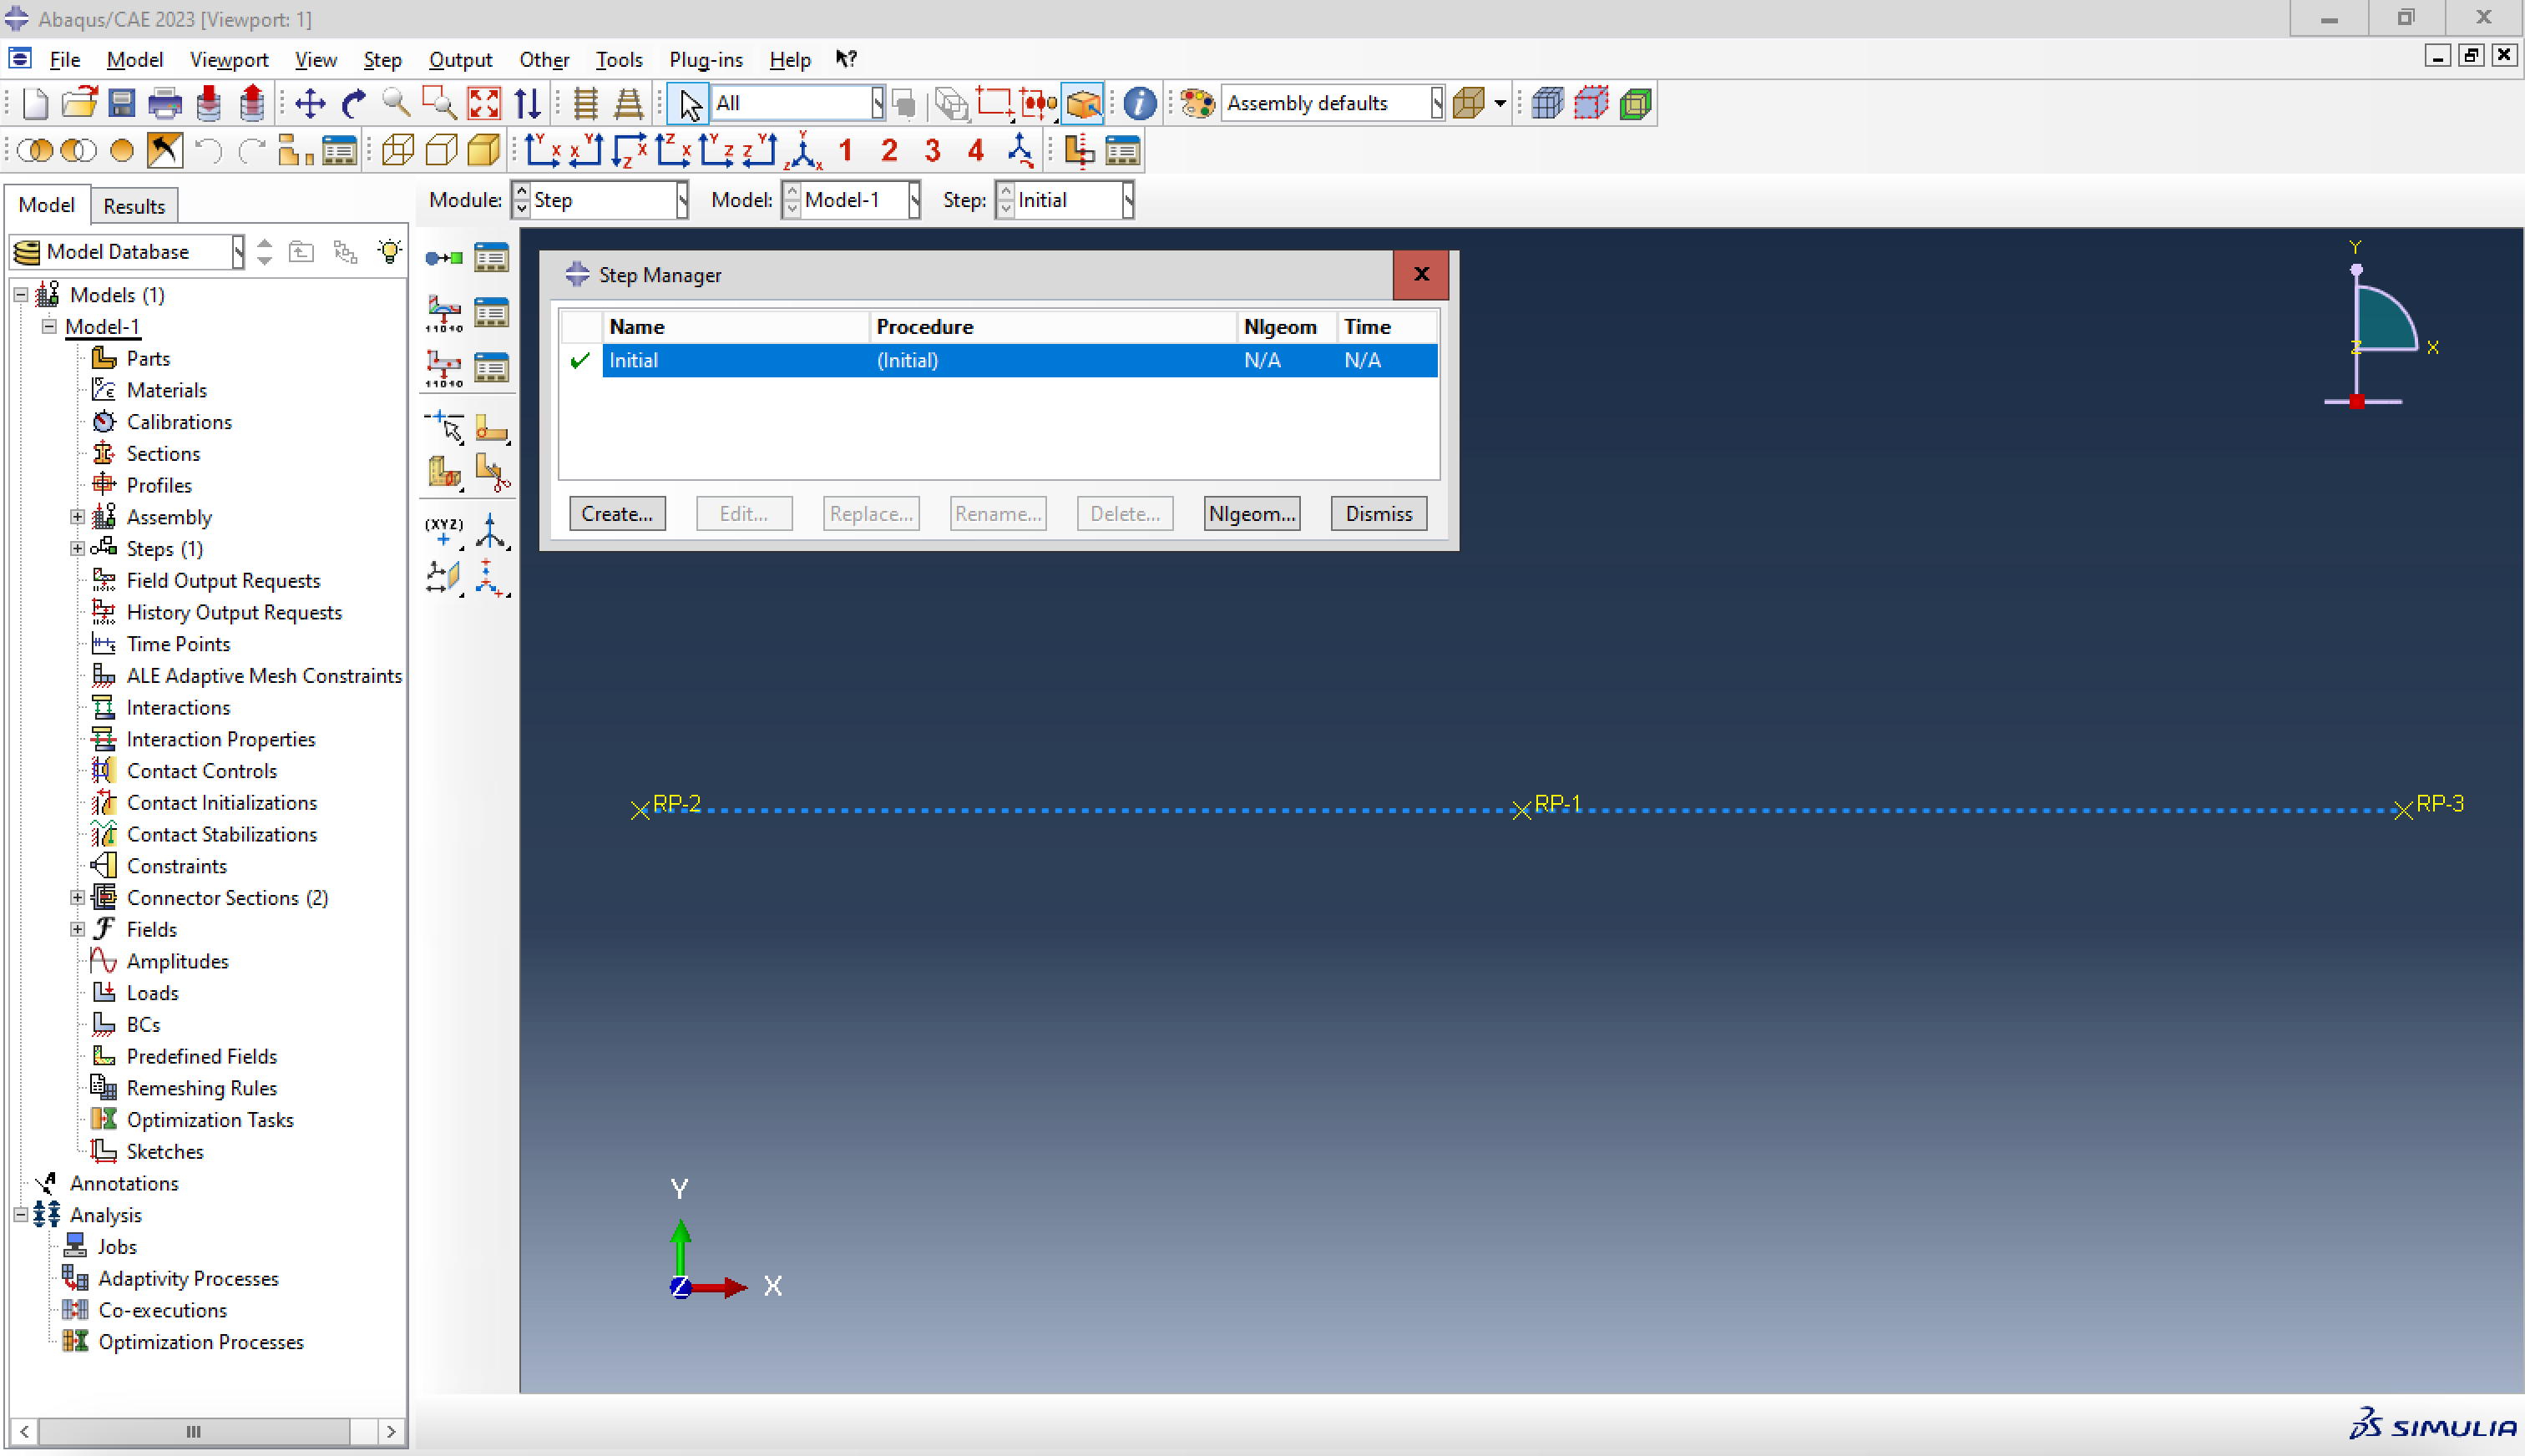
\includegraphics[width=0.9\textwidth]{Images/ab1/a12.png}
    \caption{Step Manager.}
    \label{fig:a12}
\end{figure}

and we create a new step turning on the Nlgeom option (in order to include the nonlinear effects of large displacements):
\begin{figure}[H]
    \centering
    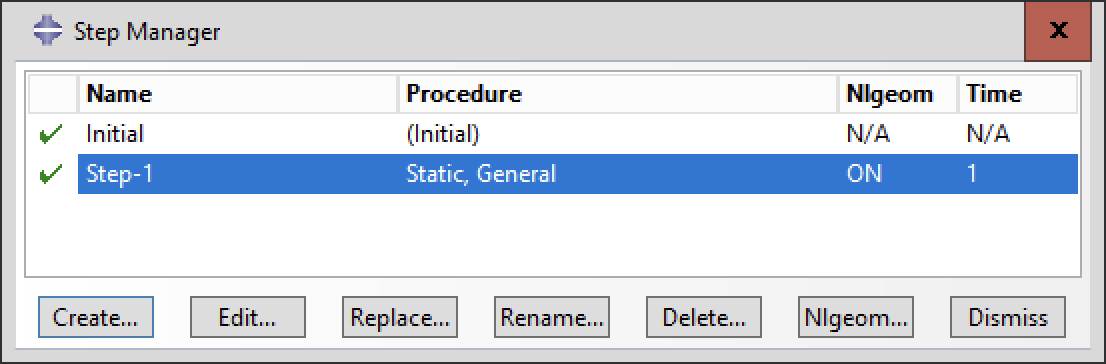
\includegraphics[width=0.4\textwidth]{Images/ab1/a13.png}
    \caption{Final result of Step module.}
    \label{fig:a13}
\end{figure}

\subsection{Load module}
\label{load_module1}%

In this module we first set the boundary conditions of the problem. For the node on the left we want to restrict the vertical, horizontal, and the out-of-plane displacements. Thus, the node on the left has U1, U2 and U3 restricted. Instead, the middle and the right nodes have just U2 and U3 restricted. Figure~\ref{fig:a14151617} shows the setting.

\begin{figure}[H]
    \centering
    \subfloat{
        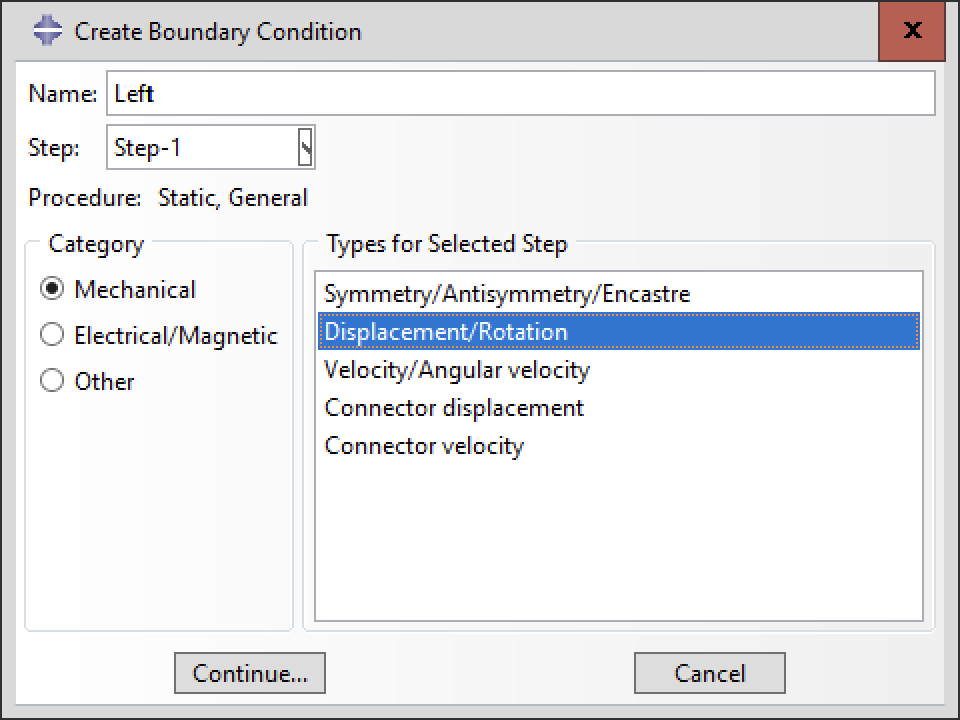
\includegraphics[scale=0.4]{Images/ab1/a14.png}
    }
    \quad
    \subfloat{
        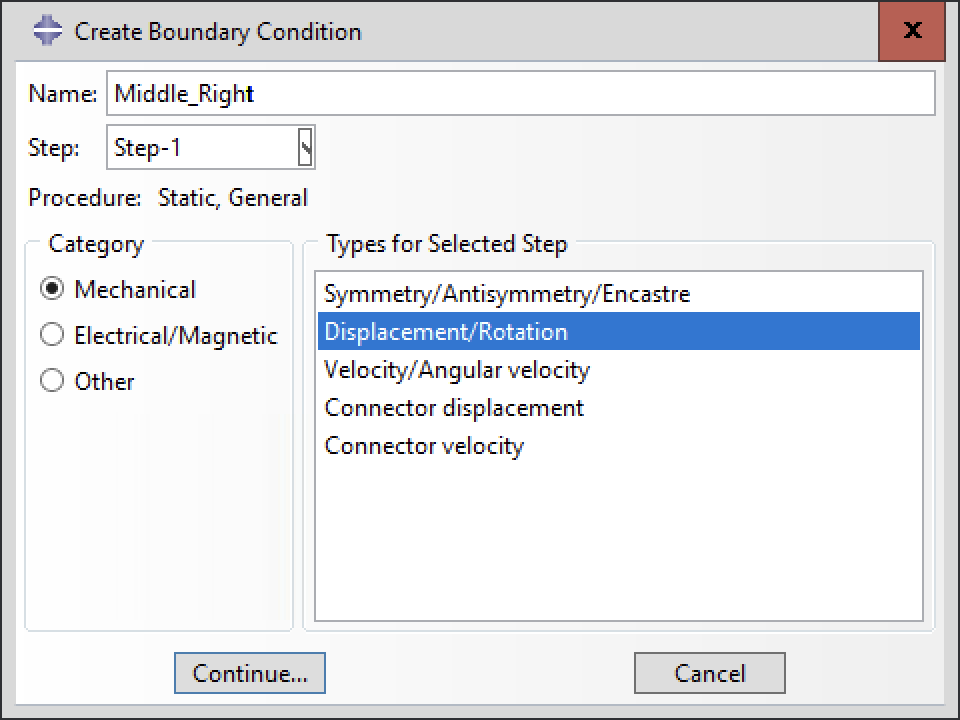
\includegraphics[scale=0.4]{Images/ab1/a16.png}
    }
    \\
    \subfloat{
        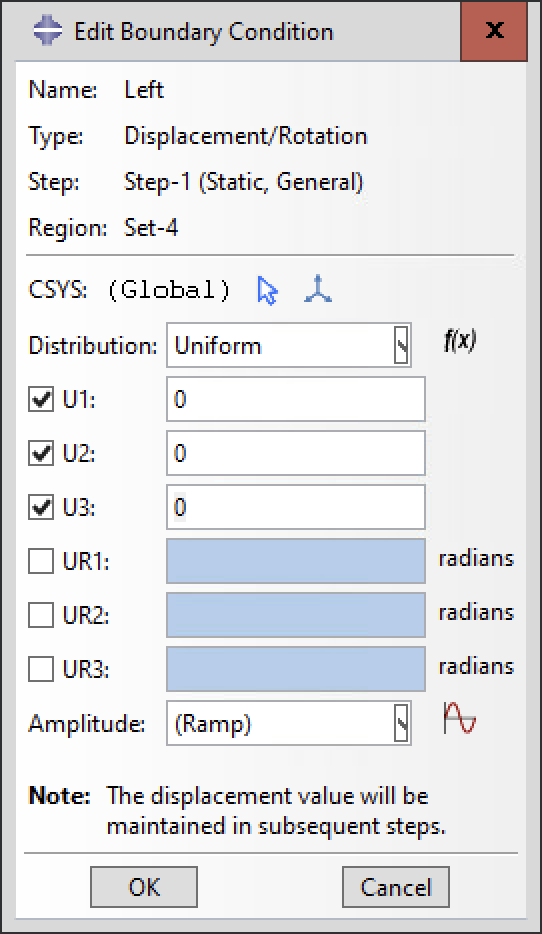
\includegraphics[scale=0.4]{Images/ab1/a15.png}
    }
    \qquad\qquad\qquad
    \subfloat{
        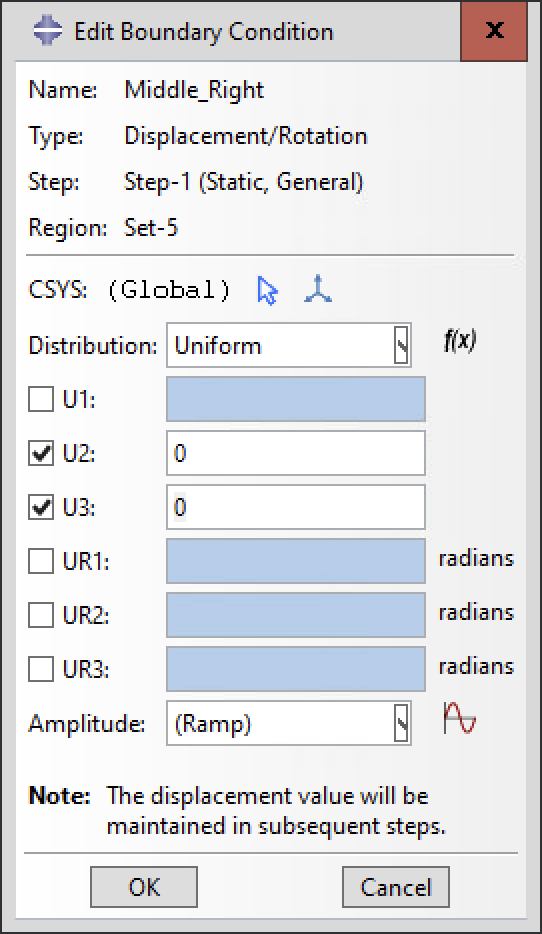
\includegraphics[scale=0.4]{Images/ab1/a17.png}
    }
    \caption{Boundary conditions of the problem.}
    \label{fig:a14151617}
\end{figure}

Then we set a concentrated force of 100 N acting on the right node in the $x$ direction with the "Create Load" symbol:
\begin{figure}[H]
    \centering
    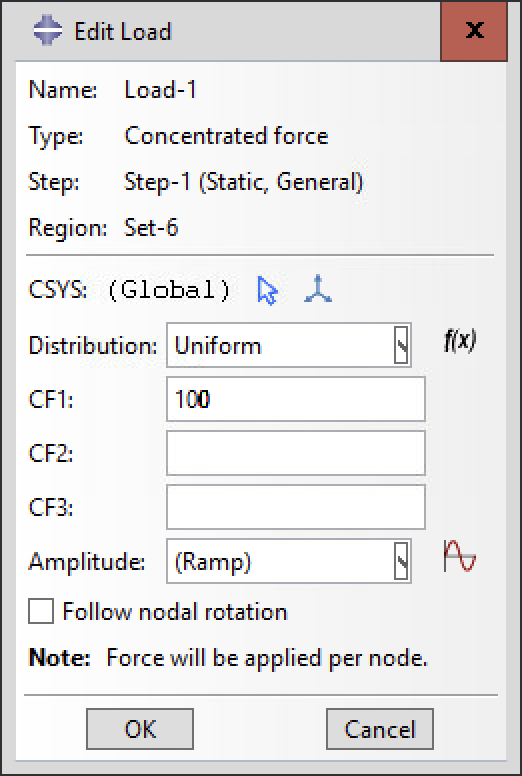
\includegraphics[width=0.25\textwidth]{Images/ab1/a20.png}
    \caption{Load options.}
    \label{fig:a20}
\end{figure}

\newpage

Here there is the result:
\begin{figure}[H]
    \centering
    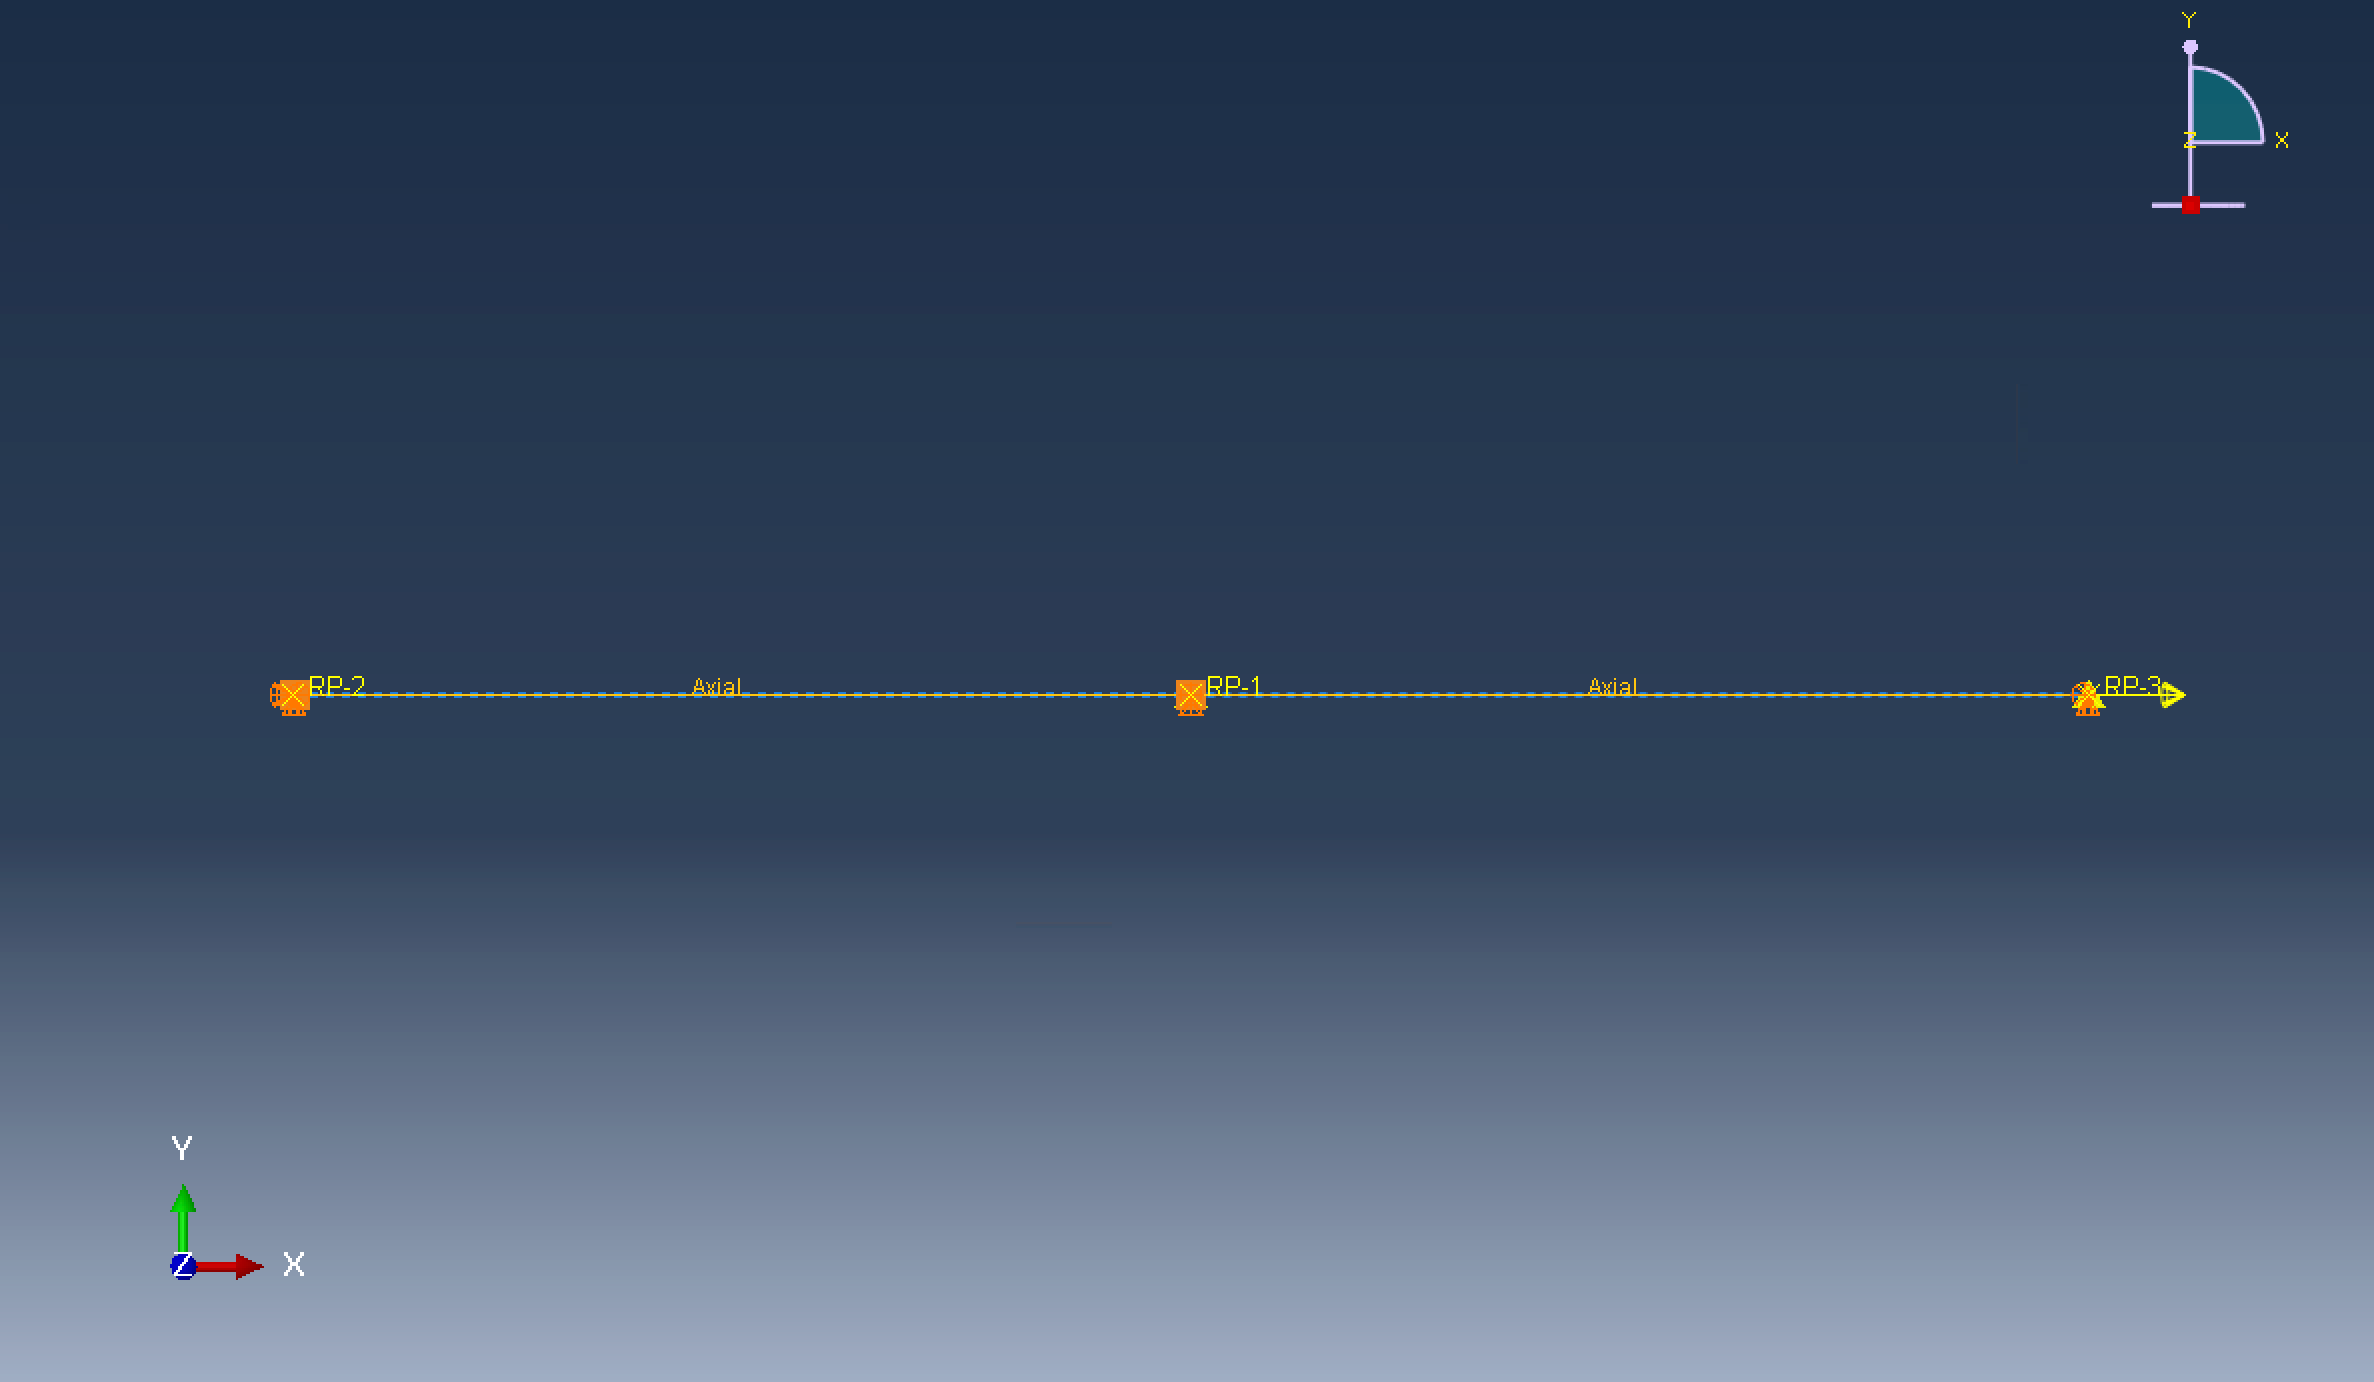
\includegraphics[width=0.9\textwidth]{Images/ab1/a21.png}
    \caption{Final result of Load module.}
    \label{fig:a21}
\end{figure}

\subsection{Job module}
\label{job_module1}%

We create a standard job in the "Job Manager" and we submit it:
\begin{figure}[H]
    \centering
    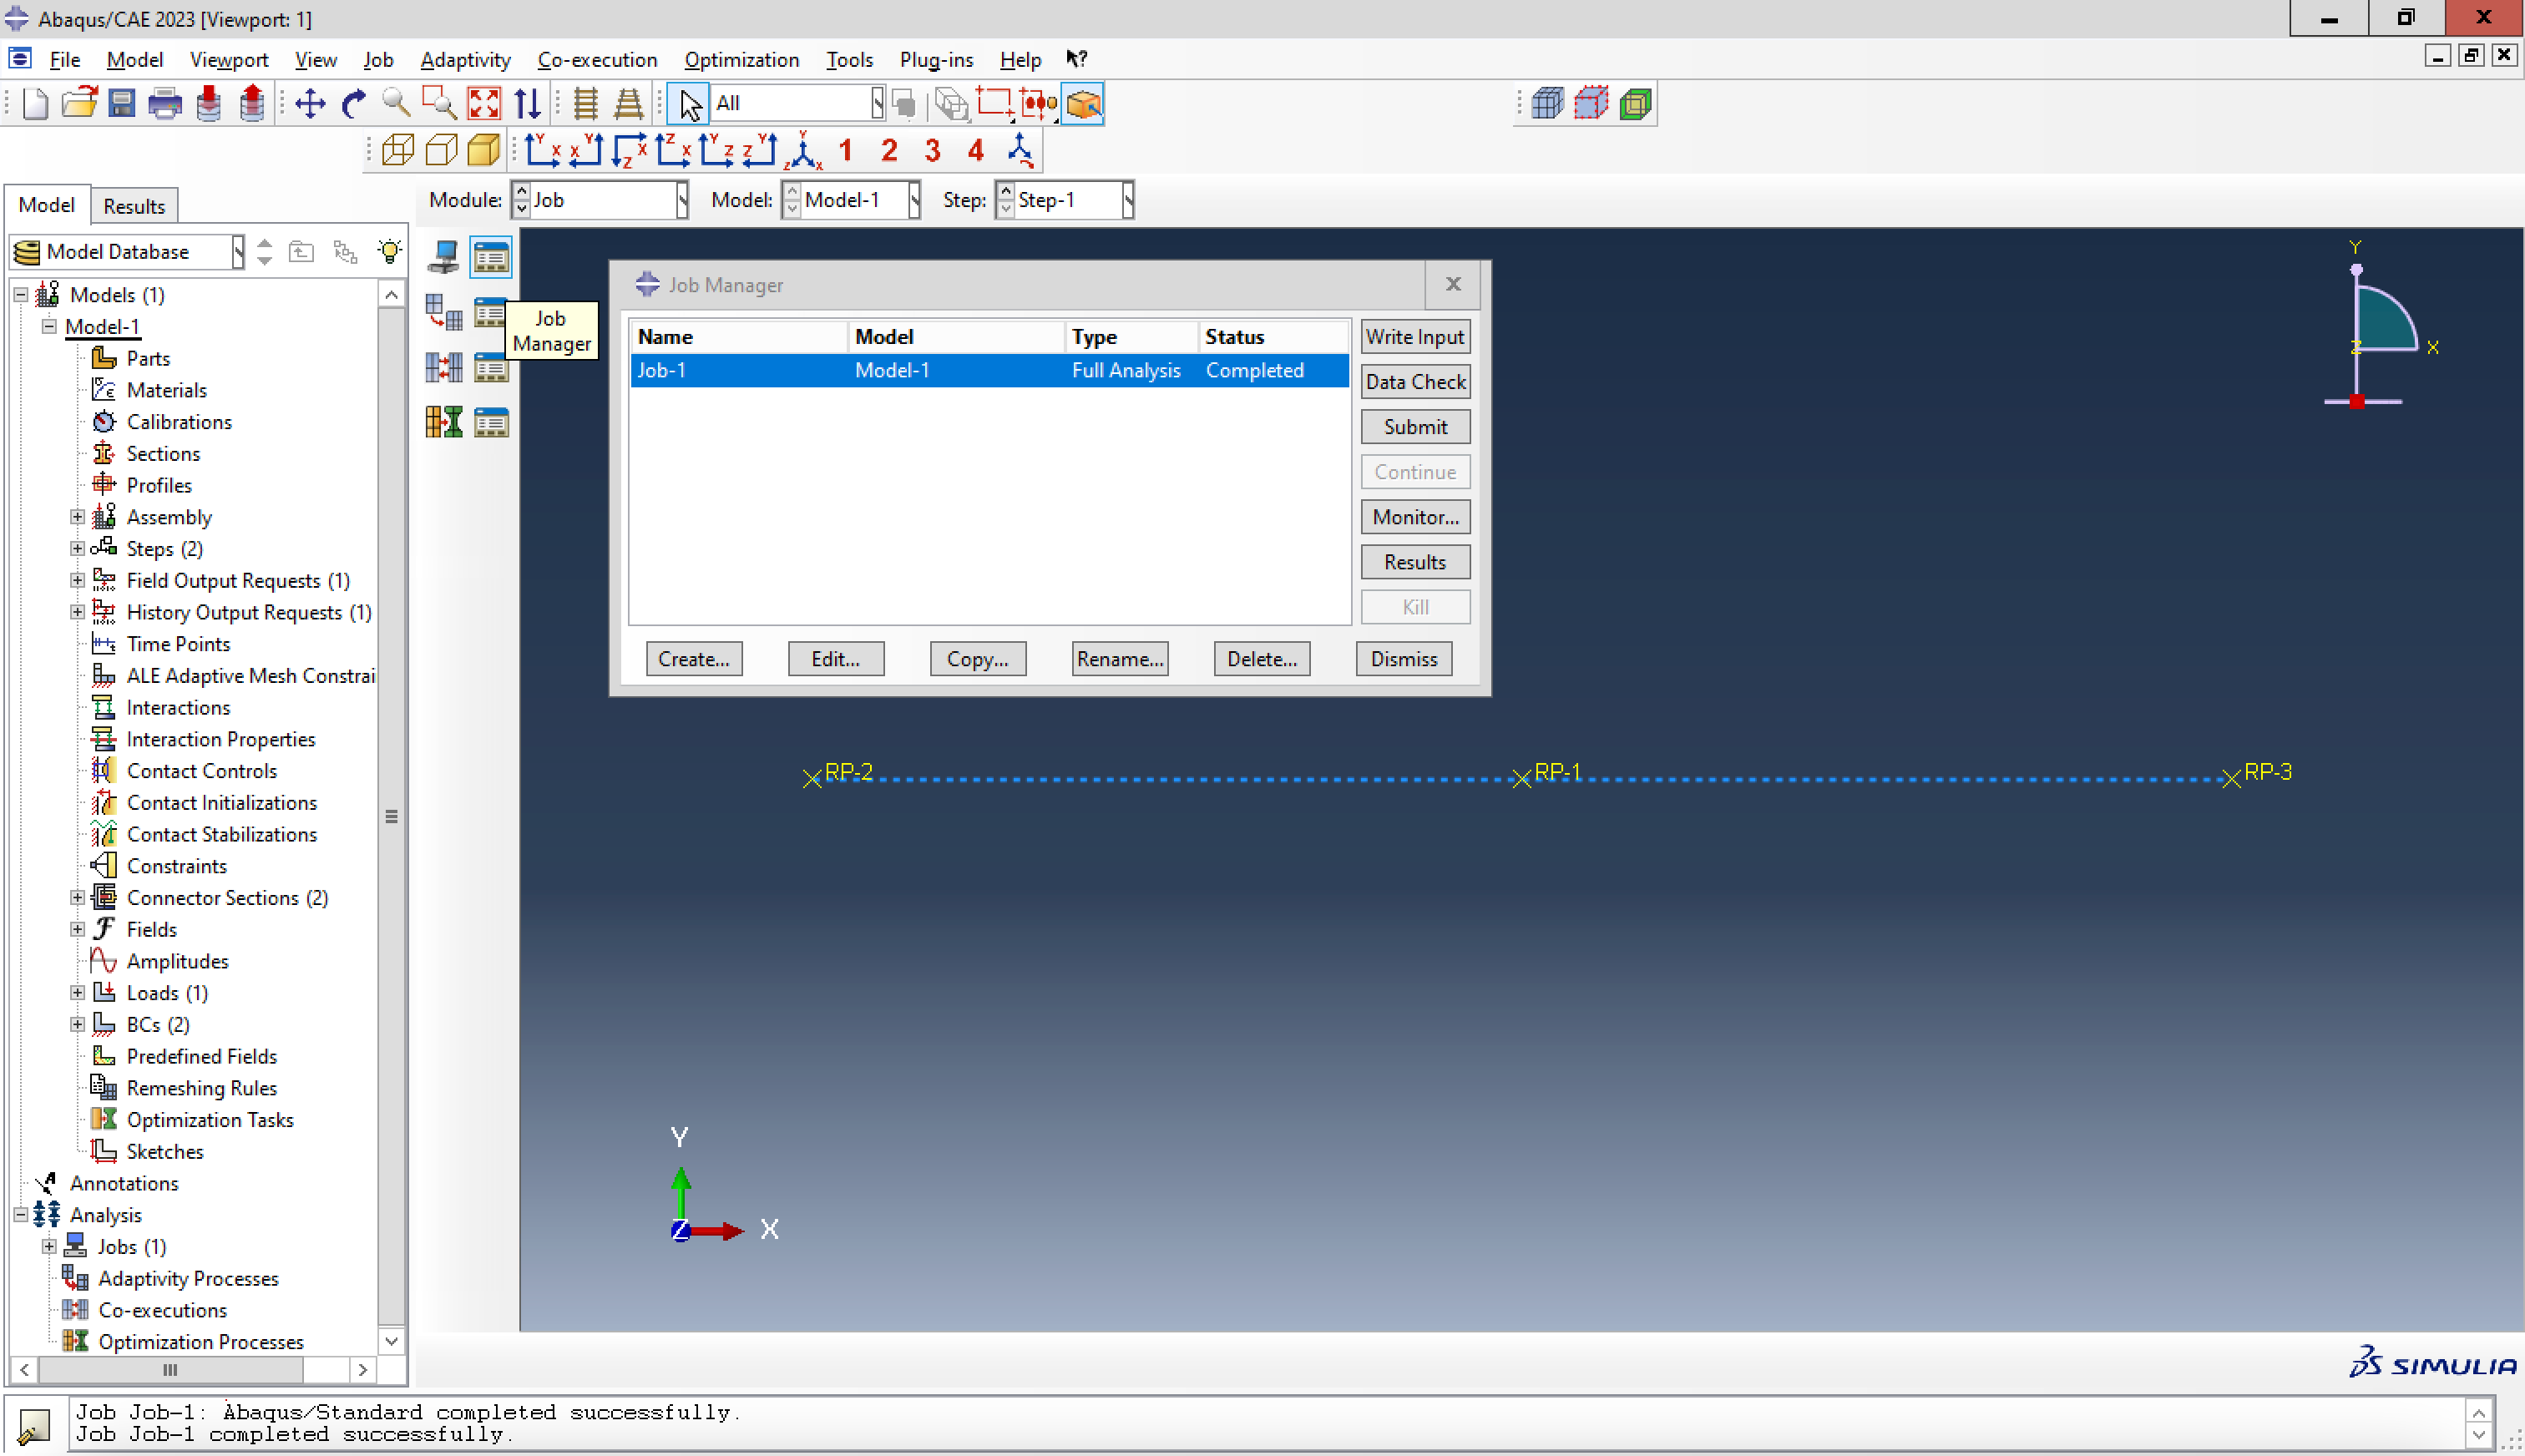
\includegraphics[width=0.9\textwidth]{Images/ab1/a23.png}
    \caption{Final result of Job module.}
    \label{fig:a23}
\end{figure}

\newpage

\subsection{Visualization module}
\label{visualization_module1}%

First, we enable the connectors view in the ODB Display Options, as in Figure~\ref{fig:a24}
\begin{figure}[H]
    \centering
    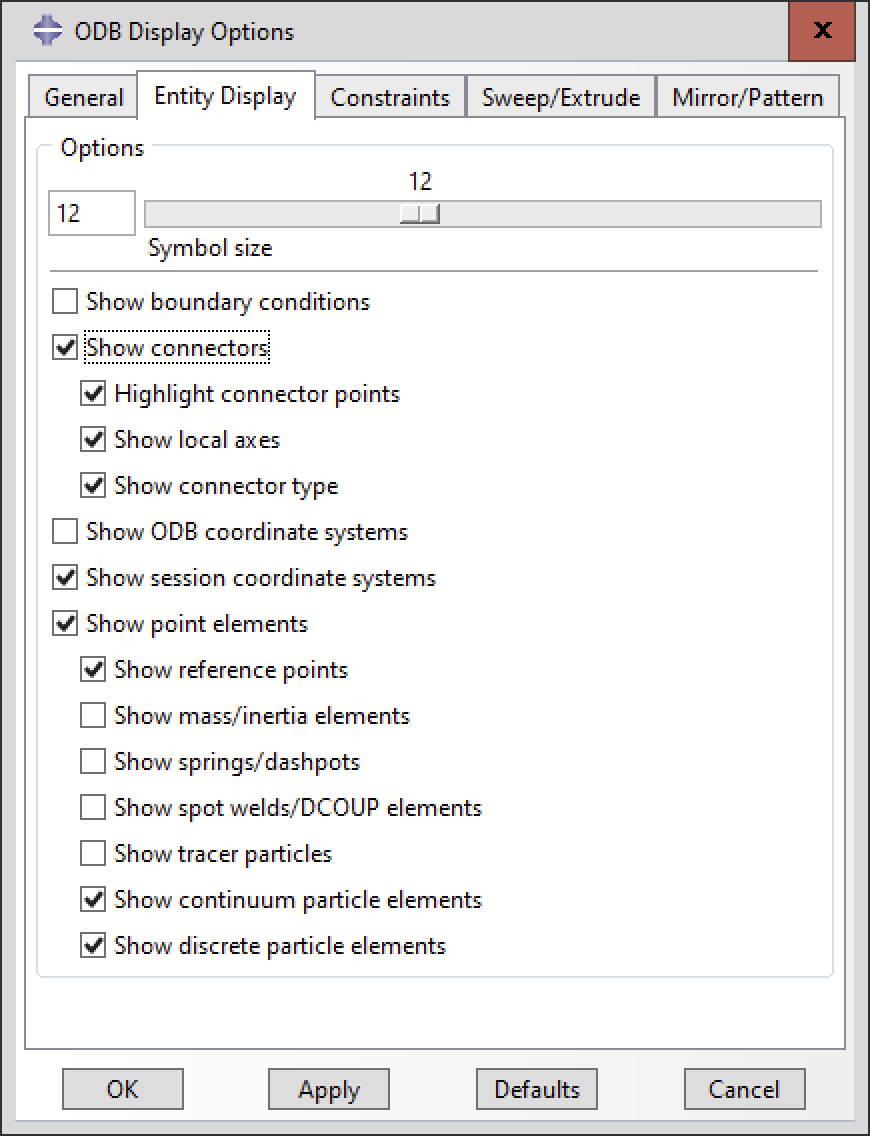
\includegraphics[width=0.3\textwidth]{Images/ab1/a24.png}
    \caption{View ODB Display Options.}
    \label{fig:a24}
\end{figure}

Here is the result we obtained:
\begin{figure}[H]
    \centering
    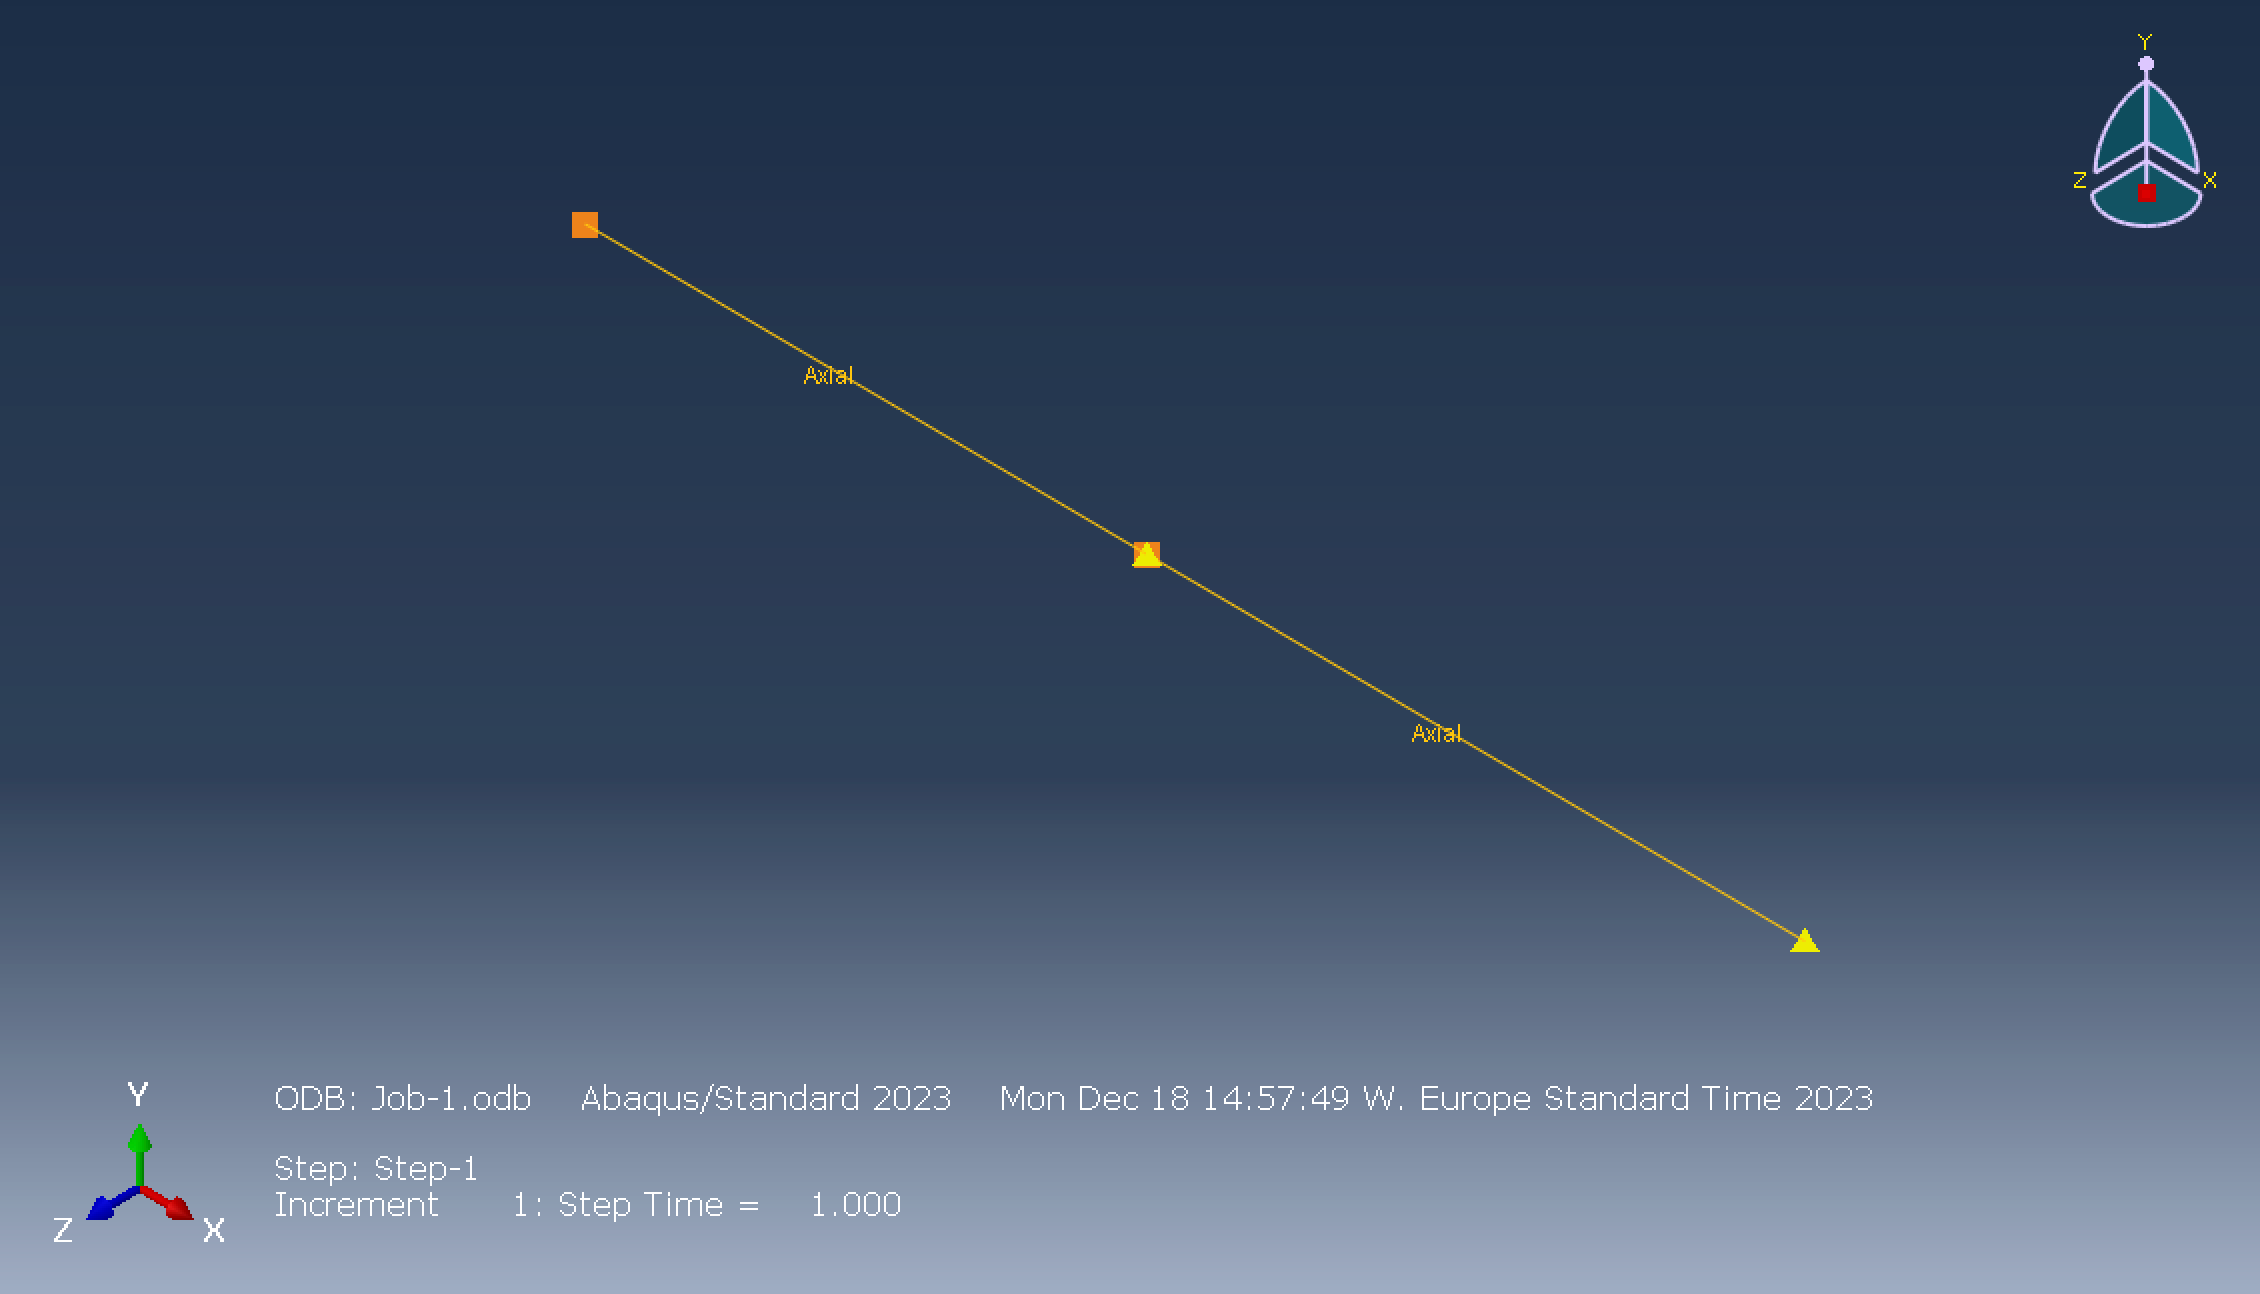
\includegraphics[width=0.9\textwidth]{Images/ab1/a25.png}
    \caption{Final result.}
    \label{fig:a25}
\end{figure}

\newpage

We can explain U1 thanks to Figure~\ref{fig:a26}.

\begin{figure}[H]
    \centering
    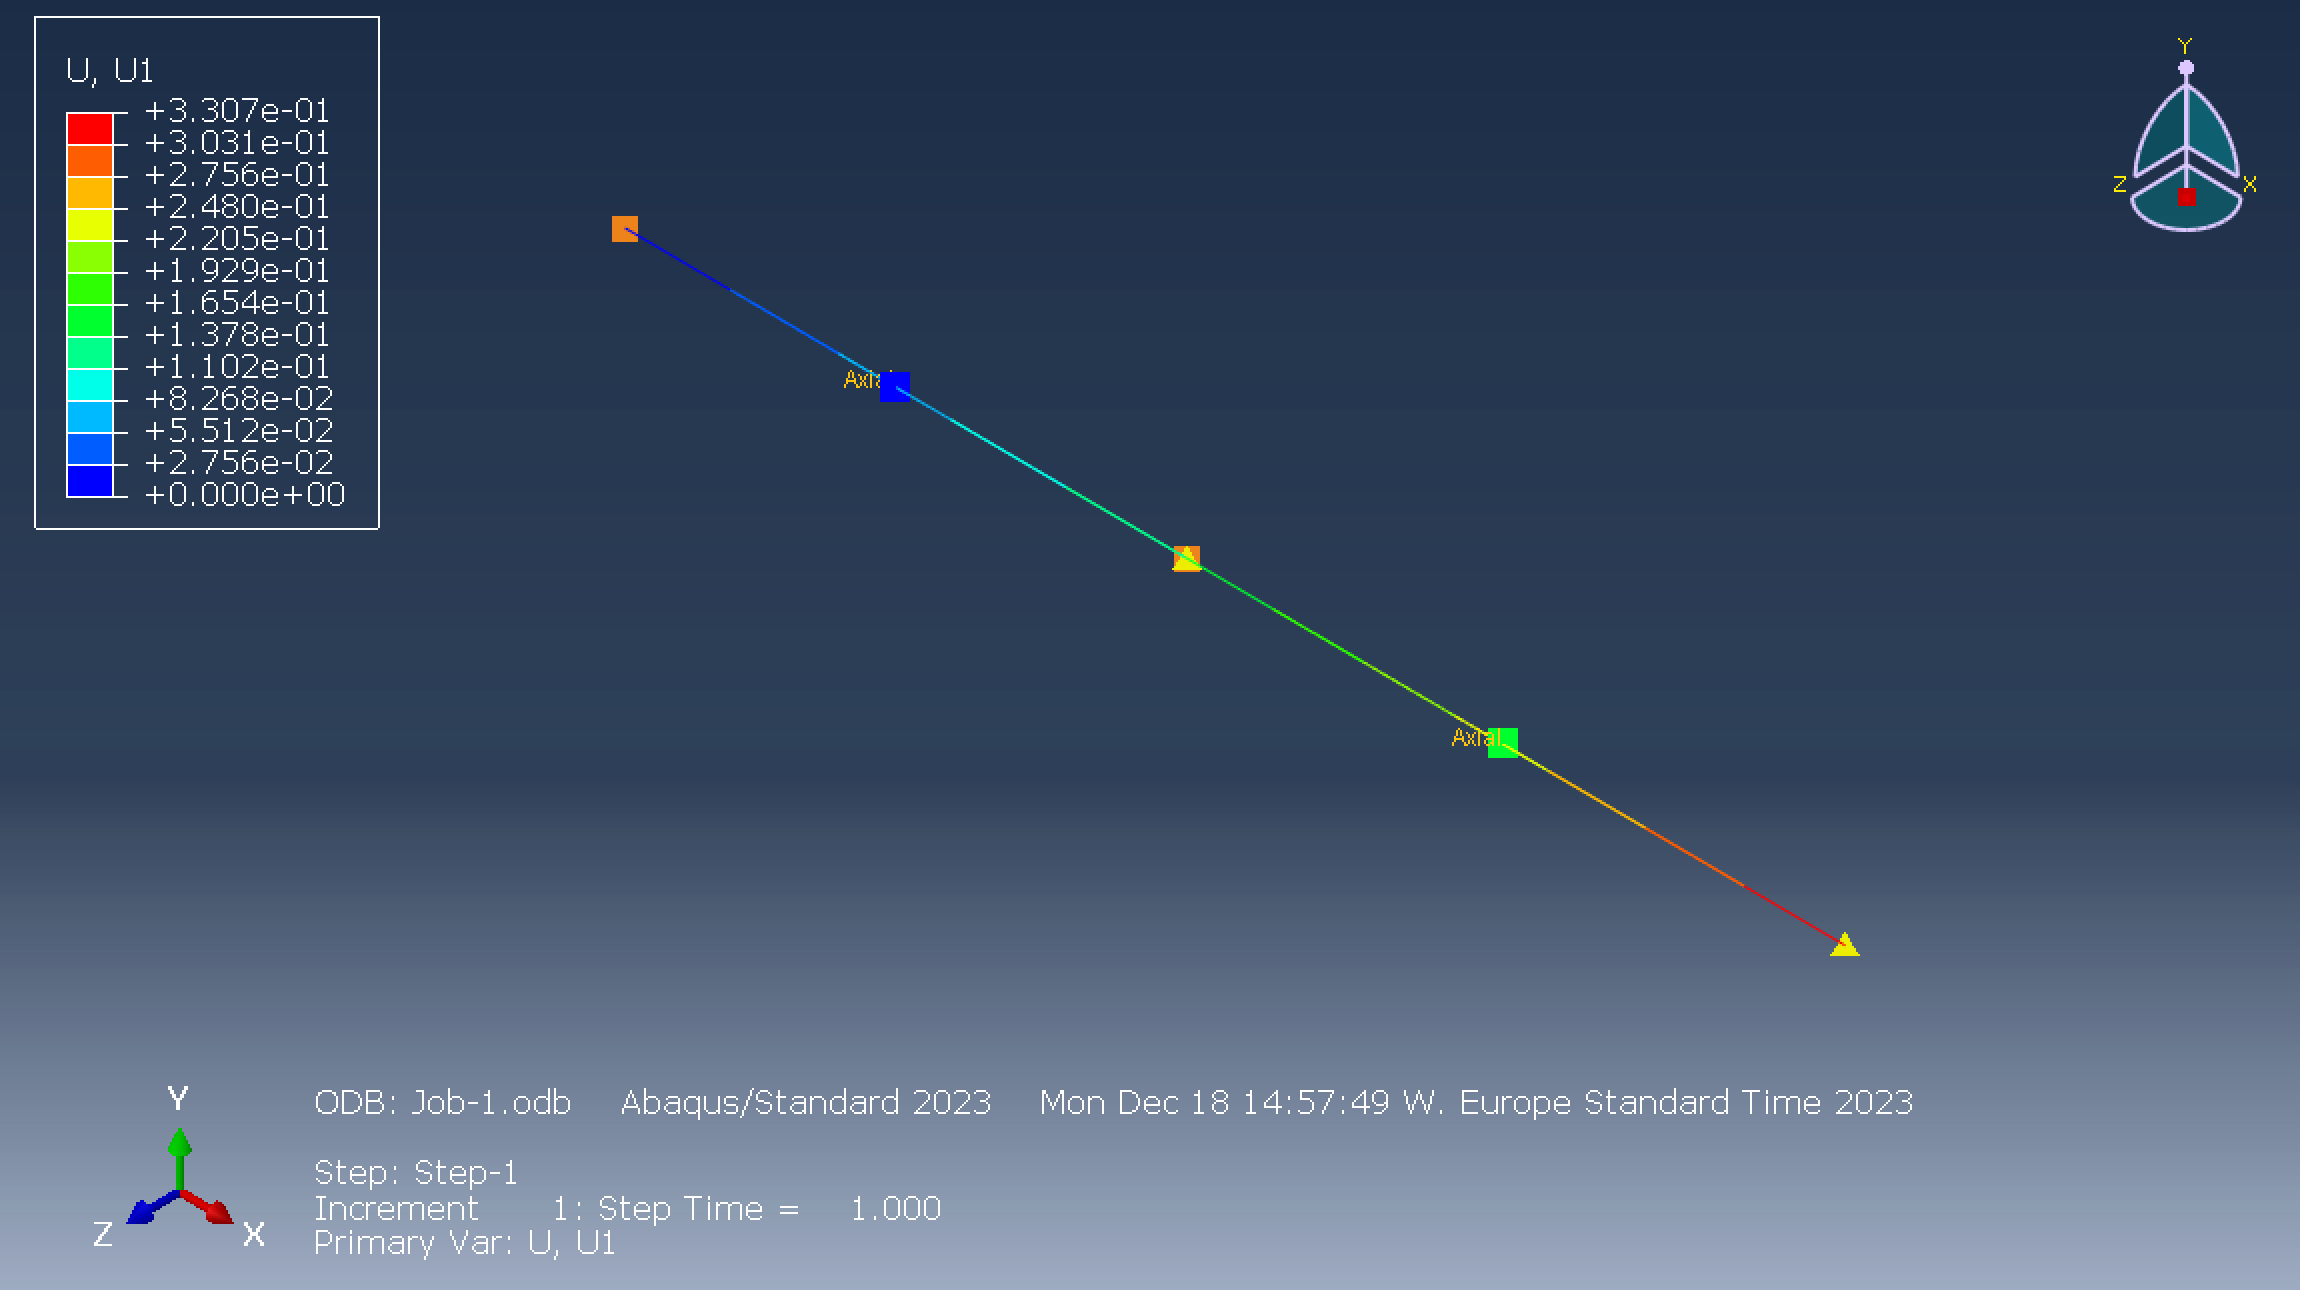
\includegraphics[width=0.9\textwidth]{Images/ab1/a26.png}
    \caption{Final result in term of U1.}
    \label{fig:a26}
\end{figure}

To be more precise, we proceed by clicking on the "Create XY Data" symbol and then we select the spatial displacement of U1 of the middle and right nodes (the ones we are interested in):
\begin{figure}[H]
    \centering
    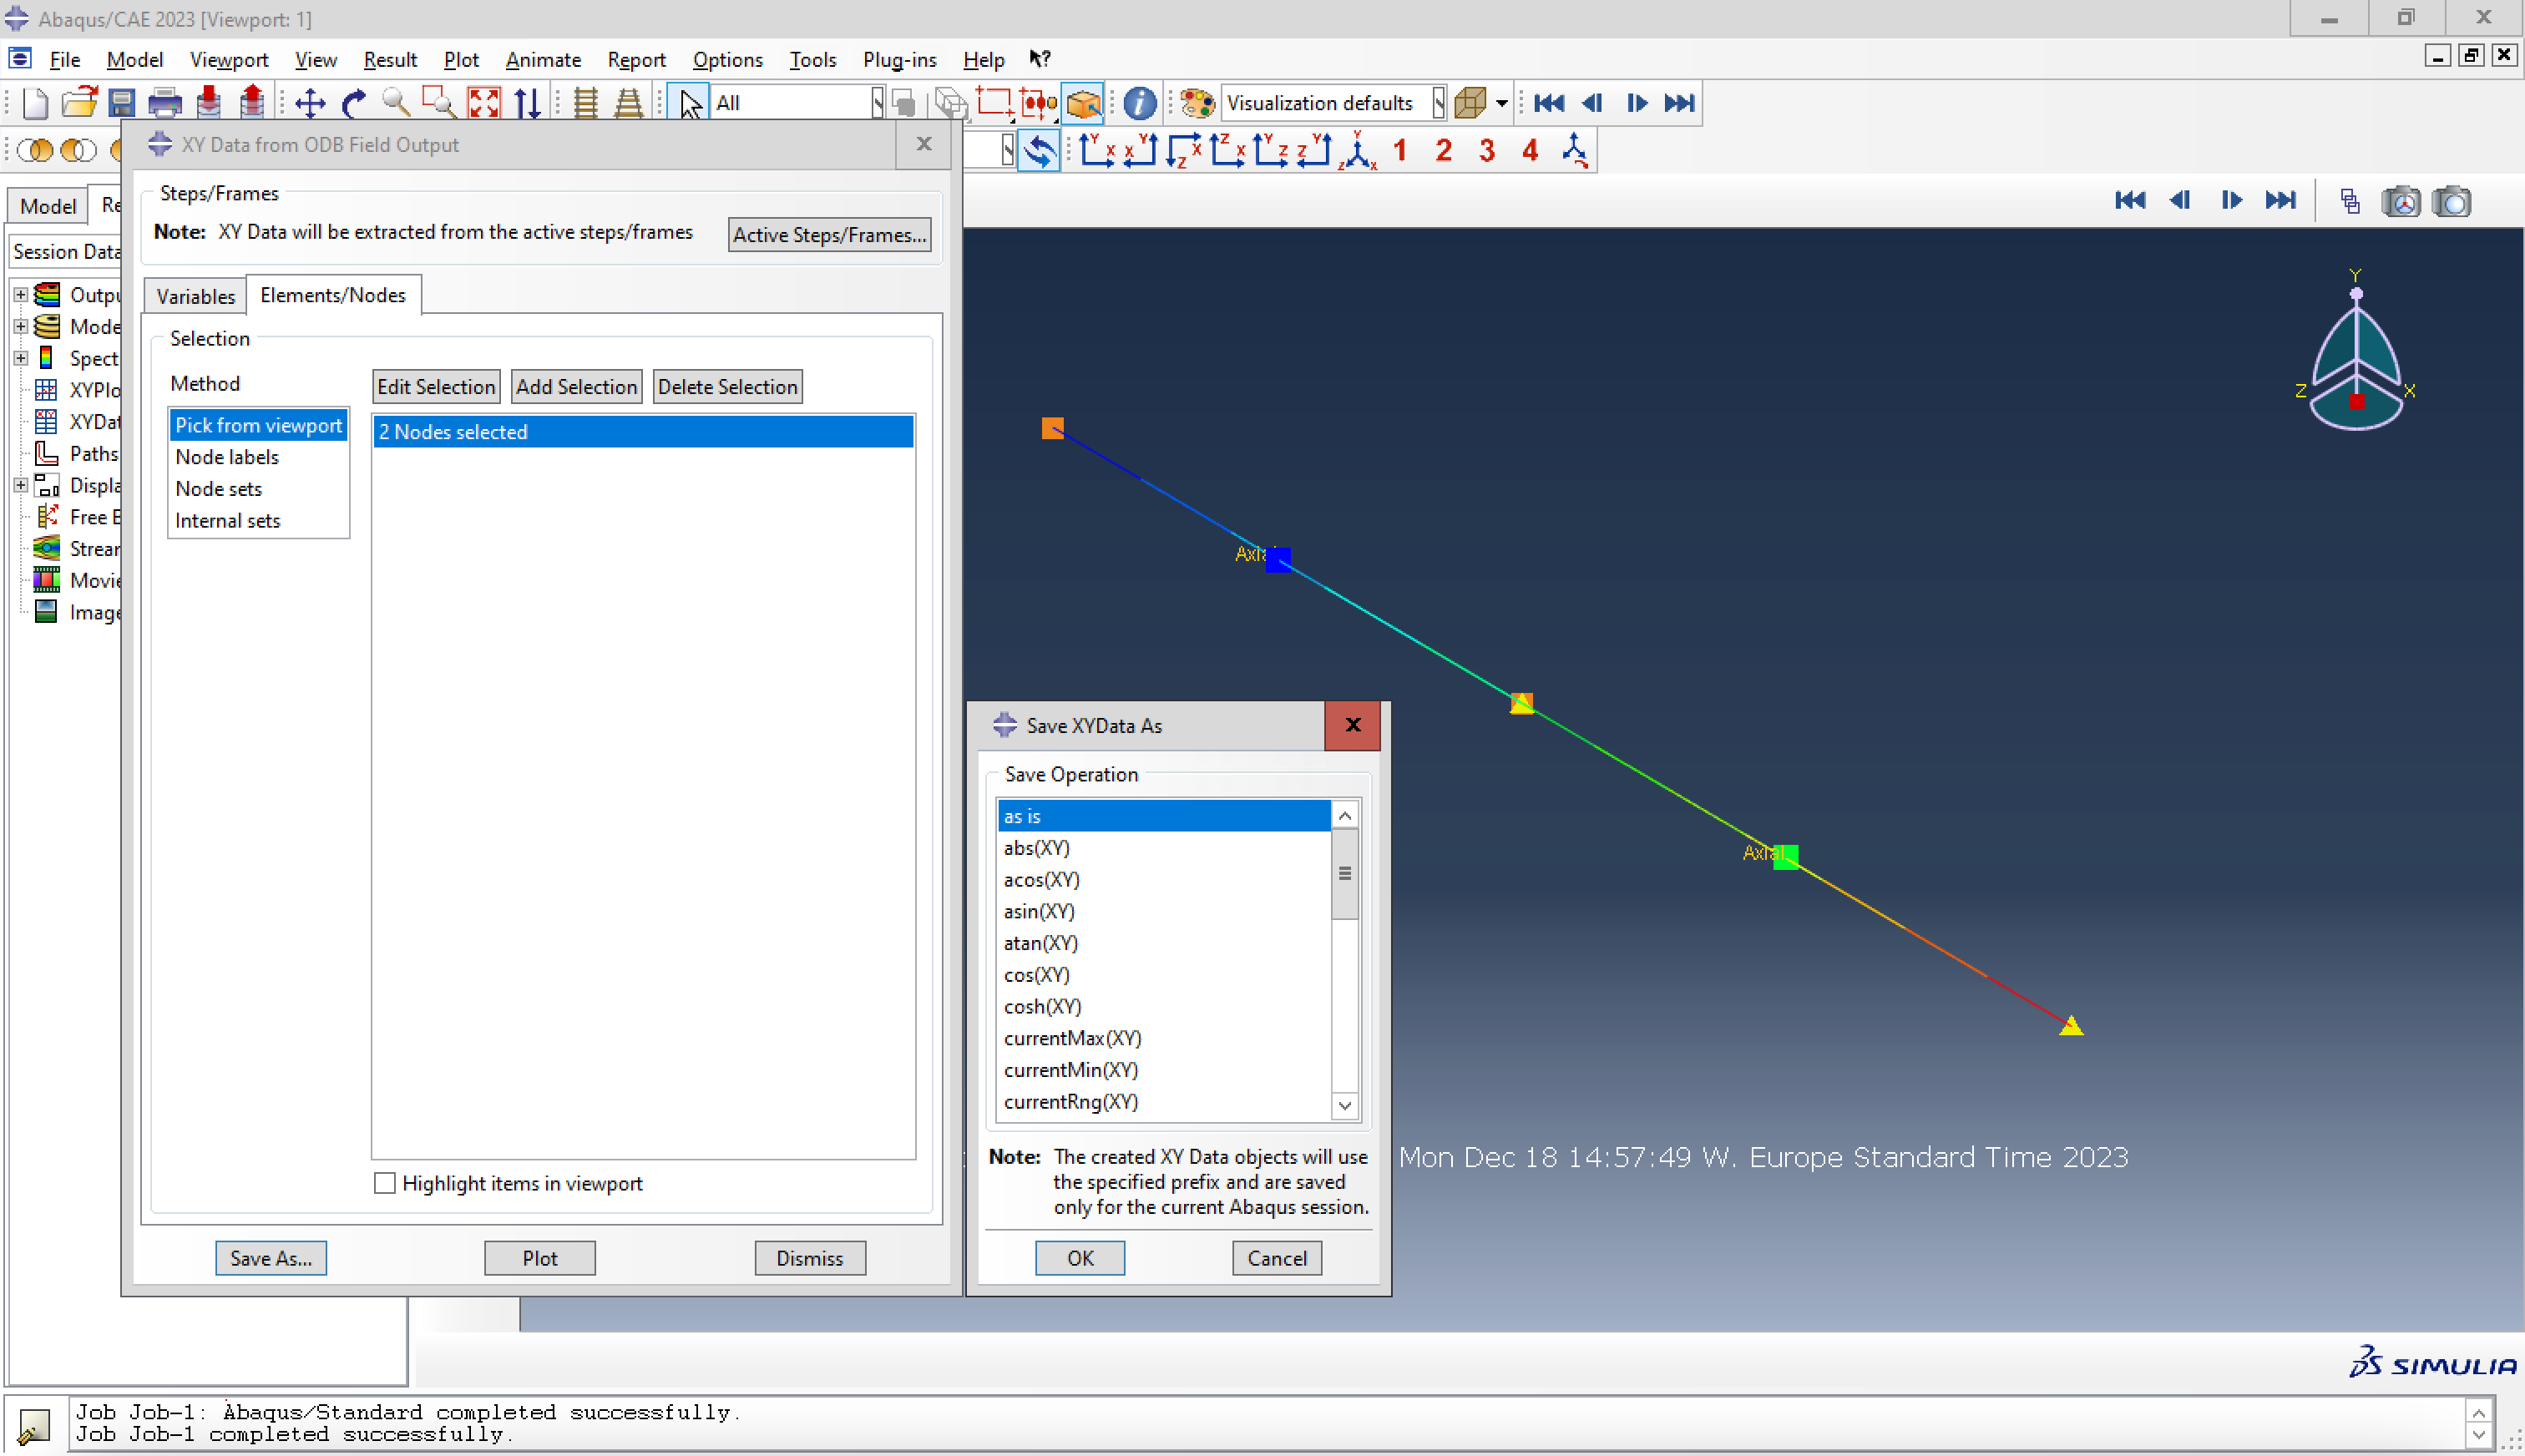
\includegraphics[width=0.9\textwidth]{Images/ab1/a29.png}
    \caption{XY Data from ODB Field Output.}
    \label{fig:a29}
\end{figure}

\newpage

Finally, by going into the \emph{edit} option of each displacement we can check the numerical result for each selected node:
\begin{figure}[H]
    \centering
    \subfloat{
        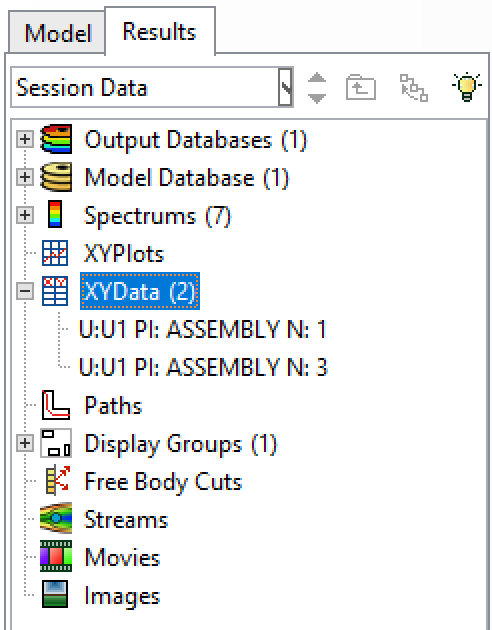
\includegraphics[scale=0.5]{Images/ab1/a30.png}
    }
    \quad
    \subfloat{
        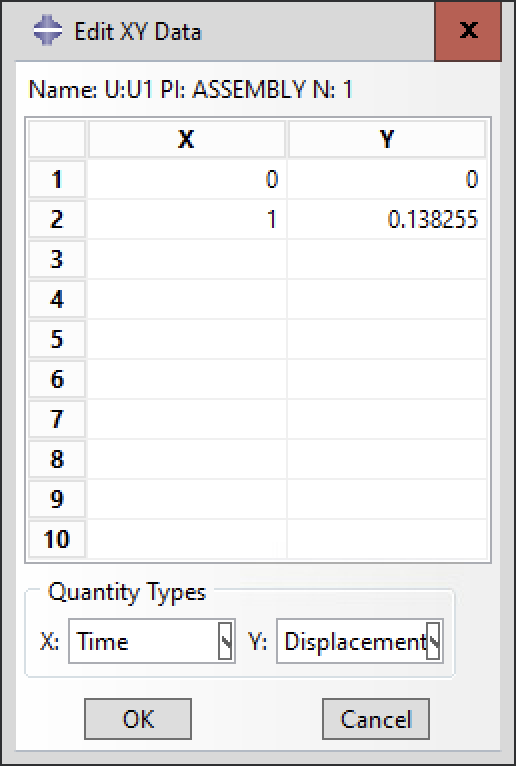
\includegraphics[scale=0.4]{Images/ab1/a31.png}
    }
    \quad
    \subfloat{
        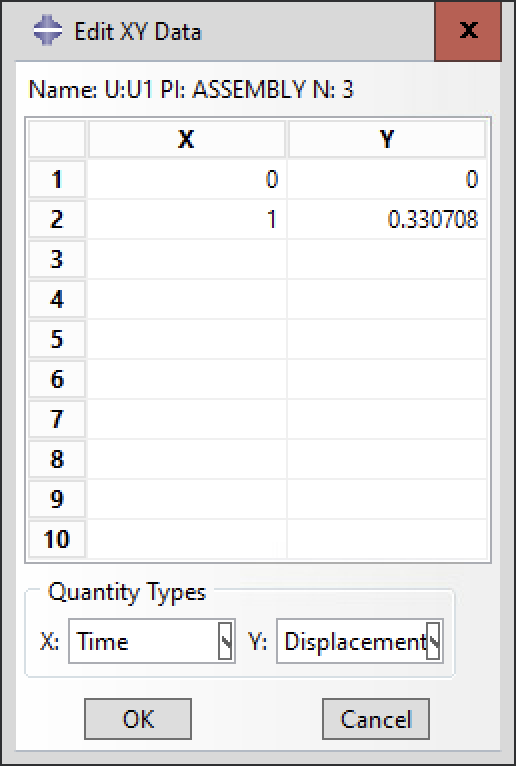
\includegraphics[scale=0.4]{Images/ab1/a32.png}
    }    
    \caption{Numerical results with Abaqus.}
    \label{fig:a303132}
\end{figure}

\section{Comparison between MATLAB and Abaqus}
\label{sec:comparison1}%

Now we compare the values previously obtained with MATLAB and Abaqus.

\begin{table}[H]
    %\caption*{\textbf{Title of Table (optional)}}
    \centering 
    \begin{tabular}{lcccc}
    \hline
    \rowcolor{bluepoli!40} % comment this line to remove the color
    Quantity & Symbol & MATLAB & Abaqus & UoM \\
    \hline
    Horizontal middle displacement & $u_1$ & 0.13873 & 0.138255 & mm \\
    Horizontal right displacement & $u_2$ & 0.33132 & 0.330708 & mm \\
    \hline
    \end{tabular}
    \\[10pt]
    \caption{MATLAB and Abaqus results.}
    \label{table:alpha_beta}
\end{table}

In conclusion, the analysis of the results obtained through simulation in MATLAB and Abaqus confirms the accuracy of the proposed model, highlighting a congruent agreement between the two software and the adopted theoretical methodology. \cleardoublepage

\chapter{Potential Problems with BEM}
\label{ch:chapter_two}%

%!TEX root = ../Thesis.tex

Hello 

\begin{table}[H]
    %\caption*{\textbf{Title of Table (optional)}}
    \centering 
    \begin{tabular}{ccccc}
    \hline
    \rowcolor{bluepoli!40} % comment this line to remove the color
    Internal Point & Name & Abaqus & MATLAB & UoM \\
    \hline
    1 & NT11 N:21 & 38.6765 & 40.00000 & °C \\
    2 & NT11 N:23 & 57.6329 & 57.88403 & °C \\
    3 & NT11 N:25 & 69.0987 & 69.15628 & °C \\
    4 & NT11 N:39 & 21.5550 & 22.11597 & °C \\
    5 & NT11 N:41 & 39.5222 & 40.00000 & °C \\
    6 & NT11 N:43 & 57.6329 & 57.88403 & °C \\
    7 & NT11 N:57 & 10.5401 & 10.84372 & °C \\
    8 & NT11 N:59 & 21.5550 & 22.11597 & °C \\
    9 & NT11 N:61 & 38.6765 & 40.00000 & °C \\
    \hline
    \end{tabular}
    \\[10pt]
    \caption{Nodal temperature results of Problem 1.}
    \label{table:stedyRes}
\end{table}

simmetria.......

\newpage

\begin{matlaboutput}
*********************************************************************
RESULTS
*********************************************************************

BOUNDARY NODES:

NODE        XM            YM            U             U_n
 1        0.12500       0.00000      80.00000     470.36316
 2        0.37500       0.00000      80.00000     116.43137
 3        0.62500       0.00000      80.00000      66.83419
 4        0.87500       0.00000      80.00000      18.38842
 5        1.00000       0.12500      80.00000      18.38842
 6        1.00000       0.37500      80.00000      66.83419
 7        1.00000       0.62500      80.00000     116.43137
 8        1.00000       0.87500      80.00000     470.36316
 9        0.87500       1.00000       0.00000    -470.36316
 10       0.62500       1.00000       0.00000    -116.43137
 11       0.37500       1.00000       0.00000     -66.83419
 12       0.12500       1.00000       0.00000     -18.38842
 13       0.00000       0.87500       0.00000     -18.38842
 14       0.00000       0.62500       0.00000     -66.83419
 15       0.00000       0.37500       0.00000    -116.43137
 16       0.00000       0.12500       0.00000    -470.36316

INTERNAL POINTS:

POINT        XIN           YIN           U
  1        0.25000       0.25000      40.00000
  2        0.50000       0.25000      57.88403
  3        0.75000       0.25000      69.15628
  4        0.25000       0.50000      22.11597
  5        0.50000       0.50000      40.00000
  6        0.75000       0.50000      57.88403
  7        0.25000       0.75000      10.84372
  8        0.50000       0.75000      22.11597
  9        0.75000       0.75000      40.00000
\end{matlaboutput} \cleardoublepage

% --------------------------------------------------------------------------

%%!TEX root = ../Thesis.tex

%% subito dopo la list of contents/figure/table/symbol section

%-------------------------------------------------------------------------
%   THESIS MAIN TEXT
%-------------------------------------------------------------------------
% In the main text of your thesis you can write the chapters in two different ways:
%
%(1) As presented in this template you can write:
%    \chapter{Title of the chapter}
%    *body of the chapter*
%
%(2) You can write your chapter in a separated .tex file and then include it in the main file with the following command:
%    \chapter{Title of the chapter}
%    \input{chapter_file.tex}
%
% Especially for long thesis, we recommend you the second option.

\addtocontents{toc}{\vspace{2em}} % Add a gap in the Contents, for aesthetics
\mainmatter % Begin numeric (1,2,3...) page numbering

% --------------------------------------------------------------------------
% NUMBERED CHAPTERS % Regular chapters following
% --------------------------------------------------------------------------
\chapter*{Introduction}

This document is intended to be both an example of the Polimi \LaTeX{} template for Master Theses,
as well as a short introduction to its use. It is not intended to be a general introduction to \LaTeX{} itself,
and the reader is assumed to be familiar with the basics of creating and compiling \LaTeX{} documents (see \cite{oetiker1995not, kottwitz2015latex}). 
\\
The cover page of the thesis must contain all the relevant information:
title of the thesis, name of the Study Programme and School, name of the author,
student ID number, name of the supervisor, name(s) of the co-supervisor(s) (if any), academic year.
The above information are provided by filling all the entries in the command \verb|\puttitle{}|
in the title page section of this template.
\\
Be sure to select a title that is meaningful.
It should contain important keywords to be identified by indexer.
Keep the title as concise as possible and comprehensible even to people who are not experts in your field.
The title has to be chosen at the end of your work so that it accurately captures the main subject of the manuscript. 
\\
Since a thesis might be a substantial document, it is convenient to break it into chapters.
You can create a new chapter as done in this template by simply using the following command
\begin{verbatim}
\chapter{Title of the chapter}
\end{verbatim}
followed by the body text.
\\
Especially for long manuscripts, it is recommended to give each chapter its own file.
In this case, you write your chapter in a separated \verb|chapter_n.tex| file
and then include it in the main file with the following command
\begin{verbatim}
\input{chapter_n.tex}
\end{verbatim}
It is recommended to give a label to each chapter by using the command
\begin{verbatim}
\label{ch:chapter_name}%
\end{verbatim}
where the argument is just a text string that you'll use to reference that part
as follows: \textit{Chapter~\ref{ch:chapter_one} contains \sc{an introduction to}  \dots}.\\
If necessary, an unnumbered chapter can be created by
\begin{verbatim}
\chapter*{Title of the unnumbered chapter}
\end{verbatim}

\chapter{Chapter one}
\label{ch:chapter_one}%
% The \label{...}% enables to remove the small indentation that is generated, always leave the % symbol.

In this chapter additional useful information are reported.

\section{Sections and subsections}
\label{sec:section_name}
Chapters are typically subdivided into sections and subsections, and, optionally,
subsubsections, paragraphs and subparagraphs.
All can have a title, but only sections and subsections are numbered.
A new section is created by the command
\begin{verbatim}
\section{Title of the section}
\end{verbatim}
The numbering can be turned off by using \verb|\section*{}|.
\\
A new subsection is created by the command
\begin{verbatim}
\subsection{Title of the subsection}
\end{verbatim}
and, similarly, the numbering can be turned off by adding an asterisk as follows 
\begin{verbatim}
\subsection*{}
\end{verbatim}

\section{Equations}
\label{sec:eqs}
This section gives some examples of writing mathematical equations in your thesis.

Maxwell's equations read:
\begin{subequations}
    \label{eq:maxwell}
    \begin{align}[left=\empheqlbrace]
    \nabla\cdot \bm{D} & = \rho, \label{eq:maxwell1} \\
    \nabla \times \bm{E} +  \frac{\partial \bm{B}}{\partial t} & = \bm{0}, \label{eq:maxwell2} \\
    \nabla\cdot \bm{B} & = 0, \label{eq:maxwell3} \\
    \nabla \times \bm{H} - \frac{\partial \bm{D}}{\partial t} &= \bm{J}. \label{eq:maxwell4}
    \end{align}
\end{subequations}

Equation~\eqref{eq:maxwell} is automatically labeled by \texttt{cleveref},
as well as Equation~\eqref{eq:maxwell1} and Equation~\eqref{eq:maxwell3}.
Thanks to the \verb|cleveref| package, there is no need to use \verb|\eqref|.
Remember that Equations have to be numbered only if they are referenced in the text.

Equations~\eqref{eq:maxwell_multilabels1}, \eqref{eq:maxwell_multilabels2}, \eqref{eq:maxwell_multilabels3}, and \eqref{eq:maxwell_multilabels4} show again Maxwell's equations without brace:
\begin{align}
    \nabla\cdot \bm{D} & = \rho, \label{eq:maxwell_multilabels1} \\
    \nabla \times \bm{E} +  \frac{\partial \bm{B}}{\partial t} &= \bm{0}, \label{eq:maxwell_multilabels2} \\
    \nabla\cdot \bm{B} & = 0, \label{eq:maxwell_multilabels3} \\
    \nabla \times \bm{H} - \frac{\partial \bm{D}}{\partial t} &= \bm{J} \label{eq:maxwell_multilabels4}.
\end{align}

Equation~\eqref{eq:maxwell_singlelabel} is the same as before,
but with just one label:
\begin{equation}
    \label{eq:maxwell_singlelabel}
    \left\{
    \begin{aligned}
    \nabla\cdot \bm{D} & = \rho, \\
    \nabla \times \bm{E} +  \frac{\partial \bm{B}}{\partial t} &= \bm{0},\\
    \nabla\cdot \bm{B} & = 0, \\
    \nabla \times \bm{H} - \frac{\partial \bm{D}}{\partial t} &= \bm{J}.
    \end{aligned}
    \right.
\end{equation}

\section{Figures, Tables and Algorithms}
Figures, Tables and Algorithms have to contain a Caption that describe their content, and have to be properly reffered in the text.

\subsection{Figures}
\label{subsec:figures}

For including pictures in your text you can use \texttt{TikZ} for high-quality hand-made figures,
or just include them as usual with the command
\begin{verbatim}
\includegraphics[options]{filename.xxx}
\end{verbatim}
Here xxx is the correct format, e.g. \verb|.png|, \verb|.jpg|, \verb|.eps|, \dots.

\begin{figure}[H]
    \centering
    
\includegraphics[width=0.3\textwidth]{logo_polimi_scritta.eps}
    \caption{Caption of the Figure to appear in the List of Figures.}
    \label{fig:quadtree}
\end{figure}

Thanks to the \texttt{\textbackslash subfloat} command, a single figure, such as Figure~\ref{fig:quadtree},
can contain multiple sub-figures with their own caption and label, e.g. \color{black} Figure~\ref{fig:polimi_logo1} and Figure~\ref{fig:polimi_logo2}. 

\begin{figure}[H]
    \centering
    \subfloat[One PoliMi logo.\label{fig:polimi_logo1}]{
        
\includegraphics[scale=0.5]{Images/logo_polimi_scritta.eps}
    }
    \quad
    \subfloat[Another one PoliMi logo.\label{fig:polimi_logo2}]{
        
\includegraphics[scale=0.5]{Images/logo_polimi_scritta2.eps}
    }
    \caption[Shorter caption]{This is a very long caption you don't want to appear in the List of Figures.}
    \label{fig:quadtree2}
\end{figure}


\subsection{Tables}
\label{subsec:tables}

Within the environments \texttt{table} and  \texttt{tabular} you can create very fancy tables as the one shown in Table~\ref{table:example}.
\begin{table}[H]
    \caption*{\textbf{Title of Table (optional)}}
    \centering 
    \begin{tabular}{|p{3em} c c c |}
    \hline
    \rowcolor{bluepoli!40} % comment this line to remove the color
     & \textbf{column 1} & \textbf{column 2} & \textbf{column 3} \T\B \\
    \hline \hline
    \textbf{row 1} & 1 & 2 & 3 \T\B \\
    \textbf{row 2} & $\alpha$ & $\beta$ & $\gamma$ \T\B\\
    \textbf{row 3} & alpha & beta & gamma \B\\
    \hline
    \end{tabular}
    \\[10pt]
    \caption{Caption of the Table to appear in the List of Tables.}
    \label{table:example}
\end{table}

You can also consider to highlight selected columns or rows in order to make tables more readable.
Moreover, with the use of \texttt{table*} and the option \texttt{bp} it is possible to align them at the bottom of the page. One example is presented in Table~\ref{table:exampleC}. 

\begin{table}[H]
\centering 
    \begin{tabular}{|p{3em} | c | c | c | c | c | c|}
    \hline
%    \rowcolor{bluepoli!40}
     & \textbf{column1} & \textbf{column2} & \textbf{column3} & \textbf{column4} & \textbf{column5} & \textbf{column6} \T\B \\
    \hline \hline
    \textbf{row1} & 1 & 2 & 3 & 4 & 5 & 6 \T\B\\
    \textbf{row2} & a & b & c & d & e & f \T\B\\
    \textbf{row3} & $\alpha$ & $\beta$ & $\gamma$ & $\delta$ & $\phi$ & $\omega$ \T\B\\
    \textbf{row4} & alpha & beta & gamma & delta & phi & omega \B\\
    \hline
    \end{tabular}
    \\[10pt]
    \caption{Highlighting the columns}
    \label{table:exampleC}
\end{table}

\begin{table}[H]
\centering 
    \begin{tabular}{|p{3em} c c c c c c|}
    \hline
%    \rowcolor{bluepoli!40}
     & \textbf{column1} & \textbf{column2} & \textbf{column3} & \textbf{column4} & \textbf{column5} & \textbf{column6} \T\B \\
    \hline \hline
    \textbf{row1} & 1 & 2 & 3 & 4 & 5 & 6 \T\B\\
    \hline
    \textbf{row2} & a & b & c & d & e & f \T\B\\
    \hline
    \textbf{row3} & $\alpha$ & $\beta$ & $\gamma$ & $\delta$ & $\phi$ & $\omega$ \T\B\\
    \hline
    \textbf{row4} & alpha & beta & gamma & delta & phi & omega \B\\
    \hline
    \end{tabular}
    \\[10pt]
    \caption{Highlighting the rows}
    \label{table:exampleR}
\end{table}

\subsection{Algorithms}
\label{subsec:algorithms}

Pseudo-algorithms can be written in \LaTeX{} with the \texttt{algorithm} and \texttt{algorithmic} packages.
An example is shown in Algorithm~\ref{alg:var}.
\begin{algorithm}[H]
    \label{alg:example}
    \caption{Name of the Algorithm}
    \label{alg:var}
    \label{protocol1}
    \begin{algorithmic}[1]
    \STATE Initial instructions
    \FOR{$for-condition$}
    \STATE{Some instructions}
    \IF{$if-condition$}
    \STATE{Some other instructions}
    \ENDIF
    \ENDFOR
    \WHILE{$while-condition$}
    \STATE{Some further instructions}
    \ENDWHILE
    \STATE Final instructions
    \end{algorithmic}
\end{algorithm} 

\vspace{5mm}

\section{Theorems, propositions and lists}

\subsection{Theorems}
Theorems have to be formatted as:
\begin{theorem}
\label{a_theorem}
Write here your theorem. 
\end{theorem}
\textit{Proof.} If useful you can report here the proof.

\subsection{Propositions}
Propositions have to be formatted as:
\begin{proposition}
Write here your proposition.
\end{proposition}

\subsection{Lists}
How to  insert itemized lists:
\begin{itemize}
    \item first item;
    \item second item.
\end{itemize}
How to insert numbered lists:
\begin{enumerate}
    \item first item;
    \item second item.
\end{enumerate}

\section{Use of copyrighted material}

Each student is responsible for obtaining copyright permissions, if necessary, to include published material in the thesis.
This applies typically to third-party material published by someone else.

\section{Plagiarism}

You have to be sure to respect the rules on Copyright and avoid an involuntary plagiarism.
It is allowed to take other persons' ideas only if the author and his original work are clearly mentioned.
As stated in the Code of Ethics and Conduct, Politecnico di Milano \textit{promotes the integrity of research,
condemns manipulation and the infringement of intellectual property}, and gives opportunity to all those
who carry out research activities to have an adequate training on ethical conduct and integrity while doing research.
To be sure to respect the copyright rules, read the guides on Copyright legislation and citation styles available
at:
\begin{verbatim}
https://www.biblio.polimi.it/en/tools/courses-and-tutorials
\end{verbatim}
You can also attend the courses which are periodically organized on "Bibliographic citations and bibliography management".

\section{Bibliography and citations}
Your thesis must contain a suitable Bibliography which lists all the sources consulted on developing the work.
The list of references is placed at the end of the manuscript after the chapter containing the conclusions.
We suggest to use the BibTeX package and save the bibliographic references  in the file \verb|Thesis_bibliography.bib|.
This is indeed a database containing all the information about the references. To cite in your manuscript, use the \verb|\cite{}| command as follows:
\\
\textit{Here is how you cite bibliography entries: \cite{knuth74}, or multiple ones at once: \cite{knuth92,lamport94}}.
\\
The bibliography and list of references are generated automatically by running BibTeX \cite{bibtex}.

\chapter{Conclusions and future developments}
\label{ch:conclusions}%
A final chapter containing the main conclusions of your research/study
and possible future developments of your work have to be inserted in this chapter. \cleardoublepage

%-------------------------------------------------------------------------
%	BIBLIOGRAPHY
%-------------------------------------------------------------------------

\addtocontents{toc}{\vspace{2em}} % Add a gap in the Contents, for aesthetics
\bibliography{Thesis_bibliography} % The references information are stored in the file named "Thesis_bibliography.bib"

%-------------------------------------------------------------------------
%	APPENDICES
%-------------------------------------------------------------------------

% LIST OF FIGURES
%\listoffigures

% LIST OF TABLES
%\listoftables

% LIST OF ALGORITHM (matlab)
%\tcblistof[\chapter*]{matalg}{List of Algorithm}

% LIST OF SYMBOLS

\cleardoublepage

\end{document}
